% Monografia para Projeto de Fim de Curso - Exemplo no LaTeX
%-----------------------------------------------------------


%---------------Inicialização de pacotes--------------------

\documentclass[12pt,a4paper,notitlepage,twoside]{book}


\usepackage{graphicx}
\usepackage[utf8]{inputenc}
\usepackage[T1]{fontenc}
\usepackage{amsmath,amssymb}
\usepackage{amsthm,amsfonts}
\usepackage{float} 
\usepackage{algorithm}
\usepackage{algpseudocode}
\usepackage{color}
\usepackage[colorlinks]{hyperref}
\usepackage{subfigure}
\usepackage{multicol}
%\usepackage[alf]{abntex2cite} %se você quiser seguir as normas ABNT no sistema autor-data
%\usepackage[num]{abntex2cite} %se você quiser seguir as normas ABNT no sistema numérico
\usepackage{setspace}
\usepackage[toc,page]{appendix}
\setlength{\parindent}{0 em}    % Paragraph indentation
\setlength{\parskip}{0.7 em}    % Space between paragraph and preceding text
\renewcommand{\baselinestretch}{1.5}    % Line spacing

%Definindo fonte Times (Use os pacotes obsoletos se não conseguir instalar os atualizados)
%\usepackage{times}     %Pacote de fontes obsoleto, apenas texto
%usepackage{mathptmx}  %Pacote de fontes obsoleto, texto e símbolos matemáticos
%\usepackage{newtxtext,newtxmath}  %Pacotes de fontes mais recentes

\usepackage[a4paper,top=30mm,bottom=30mm,inner=30mm,outer=25mm,headheight=7mm,headsep=6mm,footskip=7mm]{geometry}
\usepackage{enumerate}

\makeindex

%\singlespacing   %%espaçamento simples
%\onehalfspacing
%\setstretch{1.03} %%um pouco melhor que espaçamento simples
\linespread{1.25} %corresponde ao espaçamento 1.5 do MS Word

%---------------Início do documento-------------------------

\begin{document}

\begin{titlepage}
    \begin{center}
           
    \begin{figure}
            \centering
            % \subfigure{
\includegraphics[width=5cm]{Figuras/wac.png}}
            \hspace{0.1\textwidth}
            \subfigure{
\includegraphics[width=6cm]{Figuras/nhl-stenden.png}}
            \vspace{3cm} 
        \end{figure}

    

    {\bf\Large EHDA closed loop control system based on real time non-visual spray mode classification\\}
    \vspace{1cm} 
    {\Large Report}
    \vspace{2cm}  
    
    %\hspace{0.3\textwidth} 
    {\bf\large Student: João Pedro Miranda Marques}\\
    \vspace{2cm}
    {\large Supervisors:\\ Luewton L F Agostinho\\
            Klaus Glanzer \\
            Antônio Carrasco}
    \vspace{2cm}  

    \today
    \vspace{2cm}  
       

    %\hspace{0.3\textwidth} 
    \large \date{\today}
    \end{center}
    
    \end{titlepage}



\title{
    EHDA closed loop control system based on real time non-visual spray mode classification \\
    \large Relatório de Atividades}


\pagenumbering{roman}
\addcontentsline{toc}{chapter}{Abstract}

\begin{center}
\huge{{\bf Abstract}}
\vspace{2cm}
\end{center}

    Electrohydrodynamic Atomization (EHDA), also called electrospray, is a liquid atomization technique that
    produces micro and nanometric charged droplets within a narrow size distribution by using high electric fields (kV/cm).
    According to Cloupeau and Prunet-Foch\cite{prunet} (1994), electrosprays can generate droplets in different ways, which the authors
    named "electrospray modes". These modes may be adjusted by varying the strength of the electric field and flow rate,
    but also depend on liquid properties and system geometry. In their work, the authors proposed four possible EHDA
    modes: dripping, intermittent, cone-jet and multi-jet, which are generally distinguished visually.
    
    This project develops a closed-loop control method for EHDA devices that uses real-time, electric current-based (hence
    non-visual) spray mode classification.
    The proposed electrospray system is entirely automatic, where all the peripherals, such as HV power supply and syringe
    pump, are controlled by a computer which executes their routines.
    The system classifies spray mode dynamics using real-time current data and changes EHDA operating parameters such
    as liquid flow rate and applied voltage to achieve and maintain the chosen spray mode. The electrospray modes are
    validated in real time by using a high-speed camera.
    As compared to conventional manual approaches, the control algorithm promises higher
    accuracy and lower transient time. Therefore, a completely autonomous EHDA system opens the door to potential
    industrial applications. In addition, the use of the electric current signal can be useful to further research in electrospray
    processes, leading to better control on droplet generation (frequency, size and charge).
 

\addcontentsline{toc}{chapter}{Acknowledgment}

\begin{center}
\huge{{\bf Acknowledgments}}
\vspace{4cm}
\end{center}

I would like to express my heartfelt gratitude to the following individuals and institutions who have played a significant role in shaping me into the person I am today:

First and foremost, my beloved mother, whose support and belief in my potential has been my guiding light throughout my life. Her invaluable lessons on dedication, patience, and discipline have helped me overcome countless challenges and achieve my goals.

I also extend my gratitude to my father, whose teachings on the virtues of ambition have inspired me to strive for excellence. His relentless pursuit of success has been a constant source of energy for me.

I would like to acknowledge the outstanding education and training that I received from UFMG, which has equipped me with the necessary skills and knowledge to thrive in the global marketplace. I am grateful for the transformative experience that has prepared me for a fulfilling career and a meaningful life.

Moreover, I cannot forget my dear friends from República Casassanta, who have made my student life such a unique and unforgettable moment. Their camaraderie and support have been a source of joy and comfort during challenging times.

Lastly, I would like to thank myself for having the courage and resilience to pursue my dreams despite my anxieties and doubts. Through my perseverance, I have been able to savor every moment of my journey and give my best to achieve my goals.


\clearpage
\thispagestyle{empty}
\cleardoublepage
\tableofcontents
%\markboth{Conteúdo}{Conteúdo}

\clearpage
%\thispagestyle{empty}
%\cleardoublepage

% Normalmente, este arquivo só contém isto.
\listoffigures
\addcontentsline{toc}{chapter}{List of Figures}
%\markboth{Lista de Figuras}{Lista de Figuras}

\clearpage
%\thispagestyle{empty}
%\cleardoublepage

% Normalmente, este arquivo só contém isto.
% \listoftables
\listofalgorithms
\addcontentsline{toc}{chapter}{Lista de Tabelas}
%\markboth{Lista de Tabelas}{Lista de Tabelas}

\clearpage
%\thispagestyle{empty}
%\cleardoublepage

% Normalmente, este arquivo só contém isto.

% \tableofcontents
\pagenumbering{arabic}
\setcounter{page}{1}
\chapter{Introduction}
\label{chap:intro} 

Electrohydrodynamic Atomization (EHDA) is a way to disintegrate a liquid into droplets by exposing it to a strong electric field.\cite{prunet}
The balance between forces on the charged liquid meniscus defines the electrospraying dynamics and droplet size.
The electric current transported by the spray reveals characteristic shapes for different spray modes.
Signal processing techniques can allow a non-visual classification of the spray mode based on the electric current shape.\cite{Sjaaks}
The spray process imposes noise and random sequences on the measured signal making its classification a non-trivial task. 
Industrial applications demand automated stabilization of a spray mode. 
This can be achieved by a closed-loop control system. 
This project targets the development of a system which allows real time acquisition of the electrospray current, treat and process its values, define in which specific mode the electrospray is running and control the necessary hardware to change and/or stabilize the spray at a desired mode.


\section{Motivation and Justify}
\label{sec:motivation}

EHDA research has contributed as an important tool for the development of technology. 
The advantage of using electrospray is precision and uniform size and shape of droplets creation. 
Specially in certain spraying modes.

Although there are applications of EHDA in industry, the stabilization of the conical jet spray mode is mostly done empirically and based on average current measurements.

Many applications such as gas odorization, spray coating and pharmaceutical industries require automated stabilization of a spray mode. 
This can be achieved by a closed system loop control system. 
An automated spray mode classification is a crucial part of the control system to work, as well as the development of an appropriate control algorithm.

\section{Project Goals}
\label{sec:goals}

This project aims to give continuity to the previous student work\cite{Monica}, 
Mônica, who focused in detecting undesired discharges (sparks) in the system accusing high electric potential. 
For that, she developed a python software routine to connect most of the peripherals and analyzed the current data.
Her work corroborates the validation of this project motivating its continuation on development and optimization.

Bellow are shown the main goals listed:

\begin{enumerate}[]
\item Multipurpose applications for both scientific and industrial approaches.
\item Fully automated and intuitive system for EHDA.
\item Real time non-visual classification of electrospraying modes.
\item Control and stabilization on a desired spray. 
\item System portability and versatility.
\end{enumerate}


\section{People involved}
\label{sec:companies}

The NHL Stenden Water Technology group has been involved in previous projects that have successfully implemented automated signal processing techniques, resulting in highly ranked outcomes. 
However, further research is required to enhance the accuracy of the classification algorithm. 

In order to achieve this, the Water Technology Group at NHL Stenden University of Applied Sciences, in collaboration with Dutch companies, is conducting extensive research and implement appropriate classification algorithms. The aim is to combine analytical capabilities with infrastructure knowledge and availability to achieve optimal results.

As a student from UFMG, I am now actively involved in this research project to improve the automation usability, classification accuracy and system stabilization with signal processing techniques.

\section{Document Structure}
\label{sec:doc_struct}

This document is divided in 6 chapters. 

Chapter \ref{chap:intro} provides an introduction to EHDA and explains the inspiration behind the project.

Chapter \ref{chap:lit_review} delves into the literature concepts and knowledge that were utilized in this project.

Chapter \ref{chap:system_description} describes the system that was implemented to make this project work, along with the instruments and models used to apply our methodology.

Chapter \ref{chap:Methodology} presents the methodology applied in our experiments to validate our system.

In Chapter \ref{chap:Results}, we present our results and engage in discussions comparing the knowledge acquired through literature review.

Finally, in Chapter \ref{chap:conclusion}, we conclude our document with discussions about the goals achieved and areas for potential optimization.
\chapter{Literature Review}
\label{chap:lit_review}


\section{EHDA}
\label{sec:ehda_resume}

The electrospraying of liquids herein is referred to as electrohydrodynamic atomization (EHDA). The atomization by primarily electrical (electro) forces of a liquid (hydro) that is moving (dynamic) during the atomization captures the essence of the phenomena.\cite{Grace}
That motion applies to the liquid certain velocity that is not enough to create the spray alone. Therefore, the electric field itself is the responsible for the spraying dynamics.\cite{prunet}

The stable balance between the capillary and field forces on the liquid suggest a \emph{quasi static} dynamics.
For this reason with a controlled enviroment we can reach a certain stable spraying mode as can be seen in the Figure \ref{fig:ehda_setup_ex2}.

\begin{figure}[H]
  \centering
  \resizebox{80mm}{!}{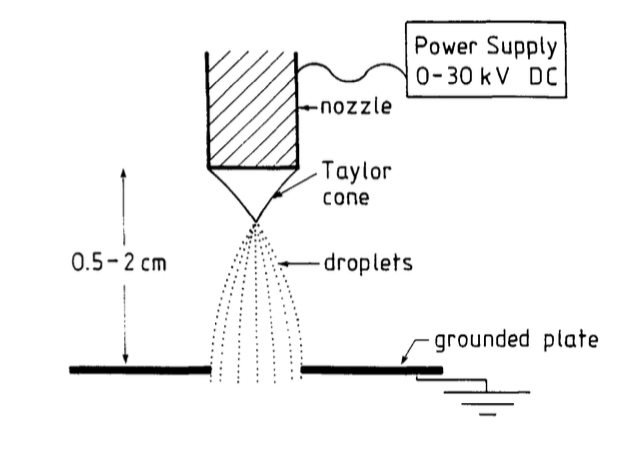
\includegraphics{Figuras/ehda_ex_2.png}}
  \caption{EHDA physical concept \cite{Gabriel}}
  \label{fig:ehda_setup_ex2}
\end{figure}


\section{Spraying modes}
\label{sec:spraying_modes_subsec}

Since 1915 with his pioneering work in EHDA, Zeleny observed several functioning modes with very different characteristics.
Years later the same phenomena was noticed by other scientists but the classification of these modes were still not well defined by the community.
For that Cloupeau and Prunet-Foch proposed spray mode classifications based in what they have seen experimentally and it's still being used as basis for EHDA researchs.\cite{prunet}

The Figures \ref{fig:dripping_camera_example}, \ref{fig:cone_camera_jet_example}, \ref{fig:multi_camera_jet_example} shows 3 spraying dynamics that we are most interesting in this project. 

\begin{multicols}{3}

  \begin{figure}[H]
      \center
      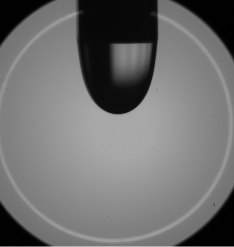
\includegraphics[width=3cm]{Figuras/drippingexample.png}
      \label{fig:dripping_camera_example}
      \caption{Dripping}
  \end{figure}


  \begin{figure}[H]
      \center
      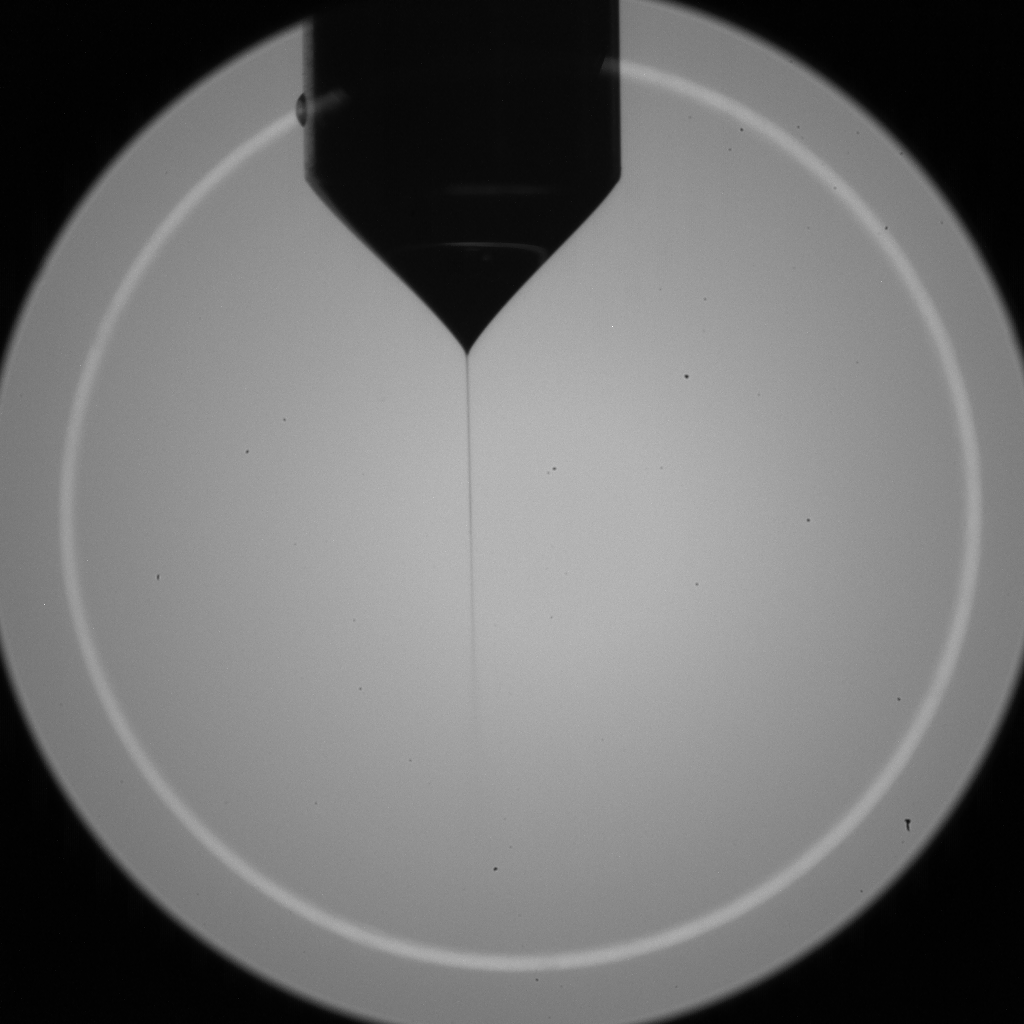
\includegraphics[width=3cm]{Figuras/conejetexample.png}
      \label{fig:cone_camera_jet_example}
      \caption{Cone Jet}
  \end{figure}


  \begin{figure}[H]
      \center
      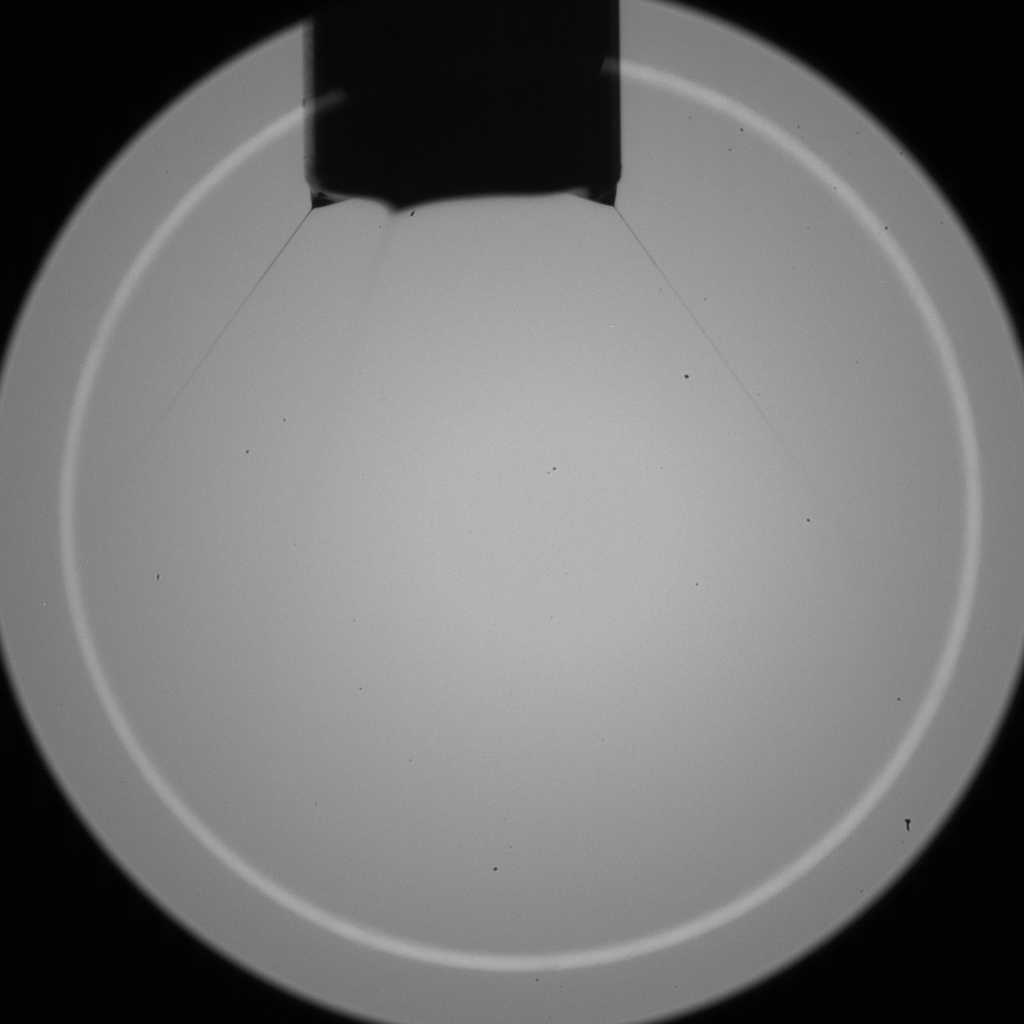
\includegraphics[width=3cm]{Figuras/multijetexample.png}
      \label{fig:multi_camera_jet_example}
      \caption{Multi Jet}
  \end{figure}

\end{multicols}


Through the various classifications and subclassifications of spraying defined in literature we are going to aggregate some of them and separate between 5 modes as shown above in order of growing electric potential:

\subsection{Dripping}
\label{subsec:dripping}

Dripping mode happens when the electric field applied is not enough to change the meniscus shape, phenomena called field enhanced dripping.
In that situation the liquid droplet has, in general, size bigger than the capillary and low frequency intervals between each drop.

\begin{figure}[H]
  \center
  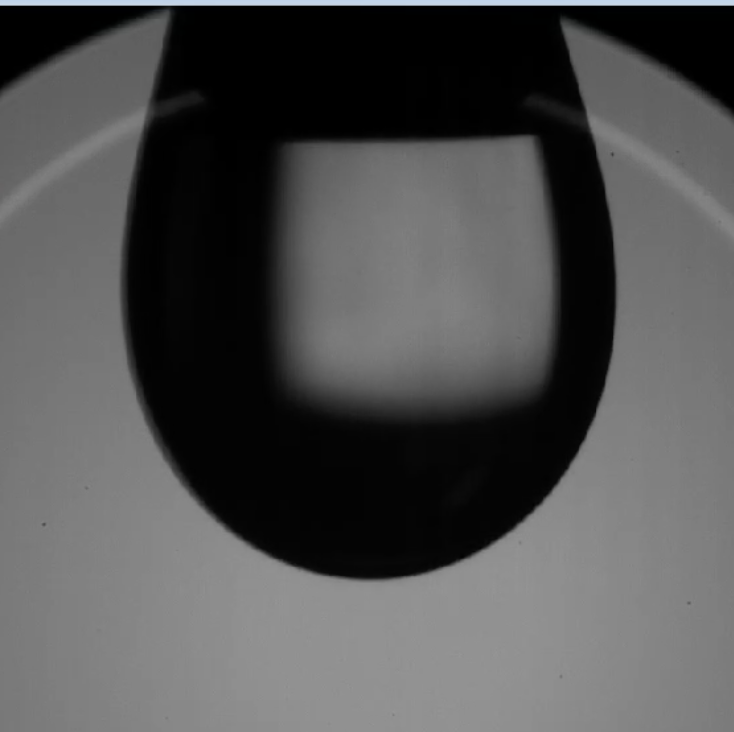
\includegraphics[width=3cm]{Figuras/19:03/drip_example.png}
  \label{fig:drip_example}
  \caption{Dripping}
\end{figure}

\subsection{Intermittent}
\label{subsec:Intermittent}

Intermittent mode is defined when the electric field forces starts to have a considerable effect in the meniscus and droplet formation. 
In this mode the droplet size is smaller than the nozzle, phenomena called microdripping, and the dripping frequency increases with the increasing of the field applied.

\begin{multicols}{3}

  \begin{figure}[H]
      \center
      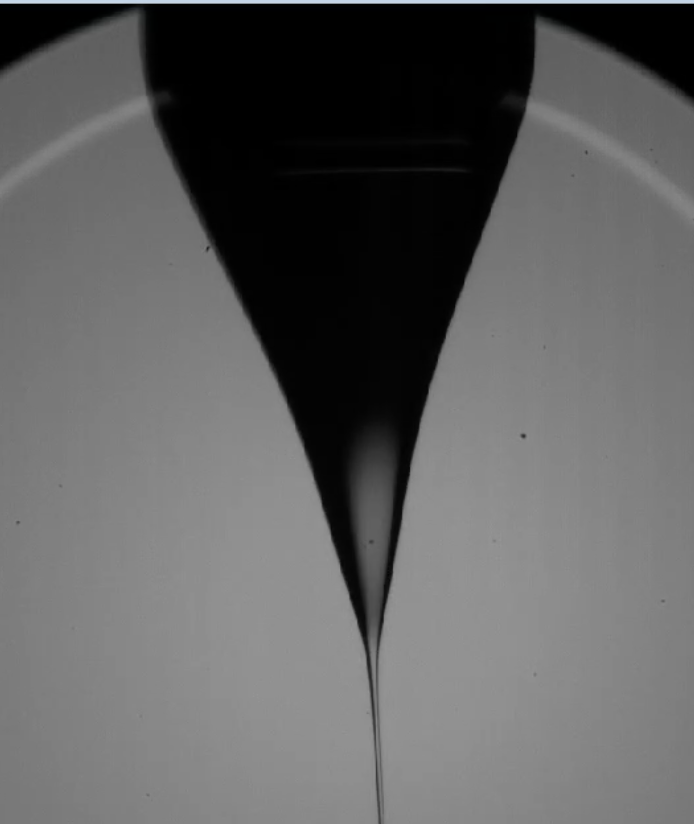
\includegraphics[width=3cm]{Figuras/19:03/intermittent_example.png}
      \label{fig:intermittent_example}
      \caption{Intermittent}
  \end{figure}


  \begin{figure}[H]
      \center
      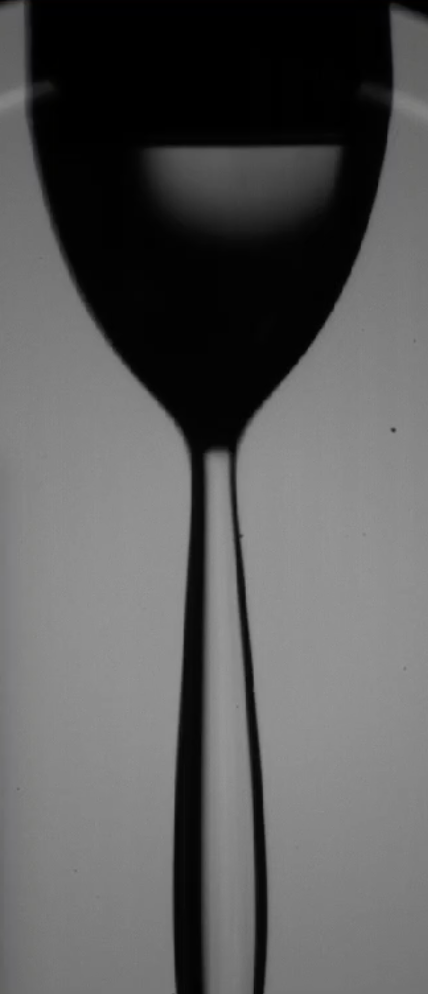
\includegraphics[width=2cm]{Figuras/19:03/intermittent2_example.png}
      \label{fig:intermittent2_example}
      \caption{Intermittent}
  \end{figure}


  \begin{figure}[H]
      \center
      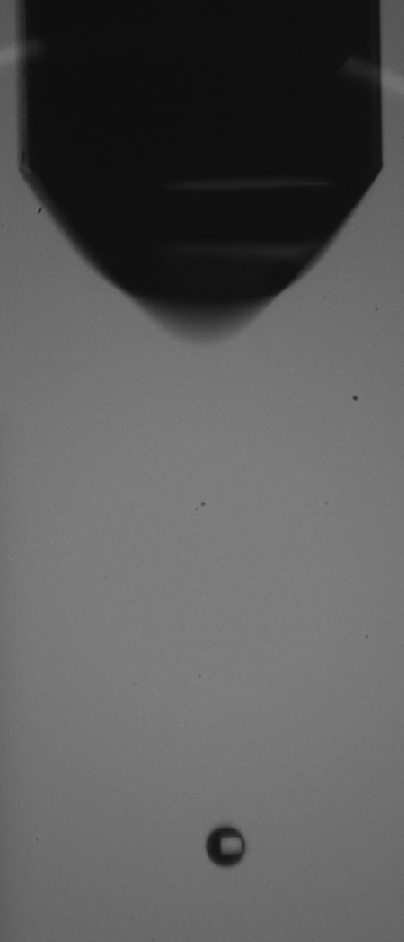
\includegraphics[width=2cm]{Figuras/19:03/microdripping_example.png}
      \label{fig:microdripping_example}
      \caption{Microdripping}
  \end{figure}

\end{multicols}

\subsection{Cone Jet}
\label{subsec:Cone Jet}

Taylor (1964) was the first to demonstrate that electrostatic pressure and capillary pressure can be balanced at any point on the surface of a liquid cone.
Taylor cone-jets naturally occurs under relatively limited circumstances: when the applied field and flow rate are in the appropriate range, and the electrosprayed liquid exhibits the adequate physical properties.

\begin{multicols}{3}

  \begin{figure}[H]
      \center
      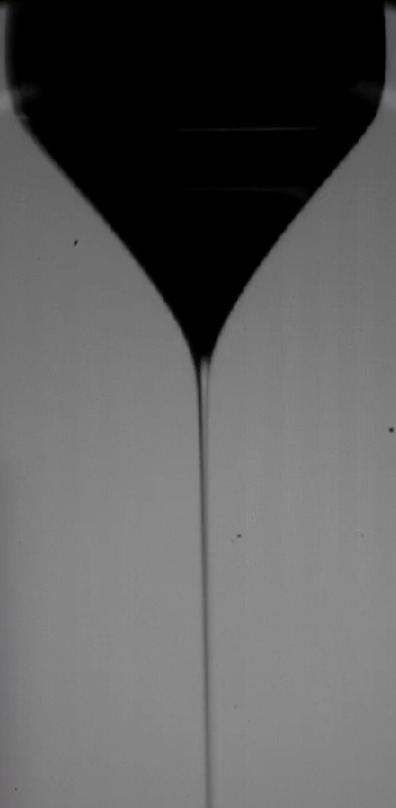
\includegraphics[width=2cm]{Figuras/april/conjet1.png}
      \label{fig:conjt1}
      \caption{Cone Jet}
  \end{figure}


  \begin{figure}[H]
      \center
      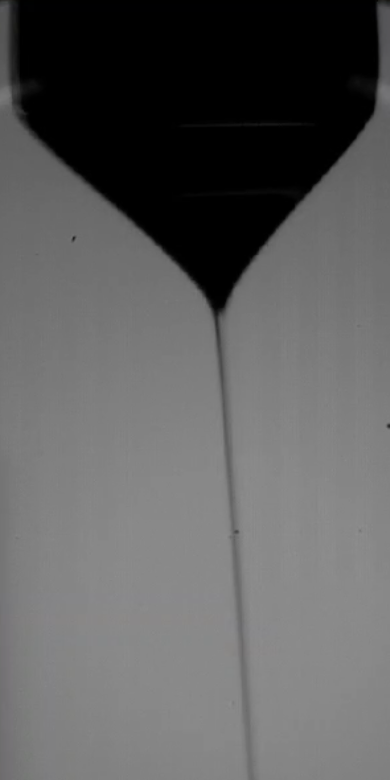
\includegraphics[width=2cm]{Figuras/april/conjet2.png}
      \label{fig:conjt2}
      \caption{Cone Jet}
  \end{figure}


  \begin{figure}[H]
      \center
      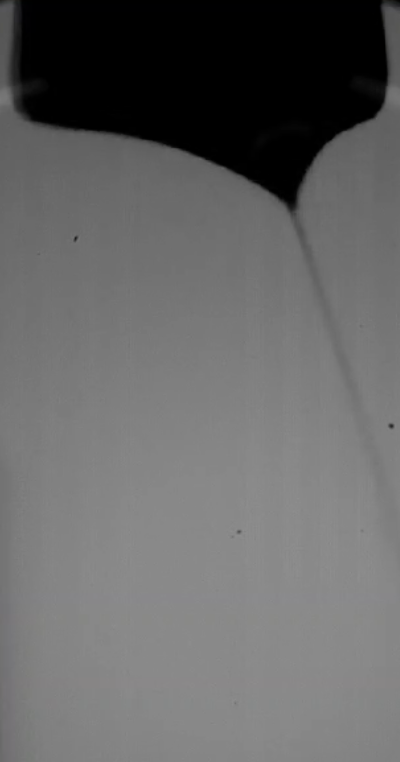
\includegraphics[width=2cm]{Figuras/april/conjet3.png}
      \label{fig:conjt3}
      \caption{Cone Jet}
  \end{figure}

\end{multicols}

\subsection{Multi Jet}
\label{subsec:Multi Jet}

\subsection{Corona sparks}
\label{subsec:Corona sparks}


\section{Non-visual classification}
\label{sec:non-visual-classification}

From the inception of EHDA until the present day, research has been carried out through manual means, involving the use of visual classification to determine the spraying mode either through cameras or by direct observation. It is advisable to employ a high-speed camera (HS) to accurately capture the spraying process as certain intermittent or dripping states may occur at a high frequency and be erroneously perceived as a stable condition.
The setup in figure \ref{fig:ehda_setup} shows the most common setup used for EHDA researchers.

\begin{figure}[H]
  \centering
  \resizebox{90mm}{!}{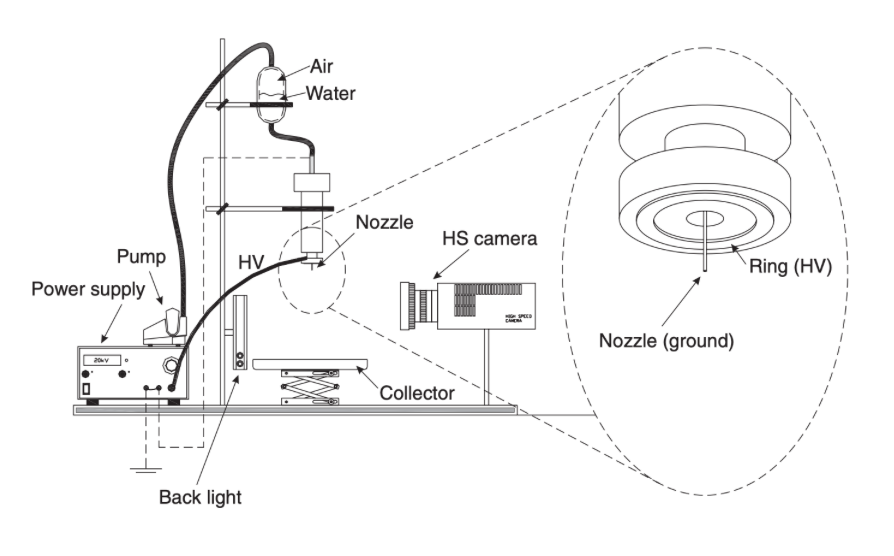
\includegraphics{Figuras/system_setup.png}}
  \caption{EHDA experiment setup \cite{Luewton}}
  \label{fig:ehda_setup}
\end{figure}


Therefore some researchs were made about the classification of the spraying mode measuring the current flowing through the nozzle to plate\cite{Sjaaks}\cite{Chen_Pui}. That current signal holds a lot o information 
about the dynamics that is happening with the liquid. Figure \ref{fig:microdripping_current_pic} illustrate an example of that. It can be seen the signal of two droplets of charged liquid generated in this time frame.


\begin{figure}[H]
    \centering
    \resizebox{150mm}{!}{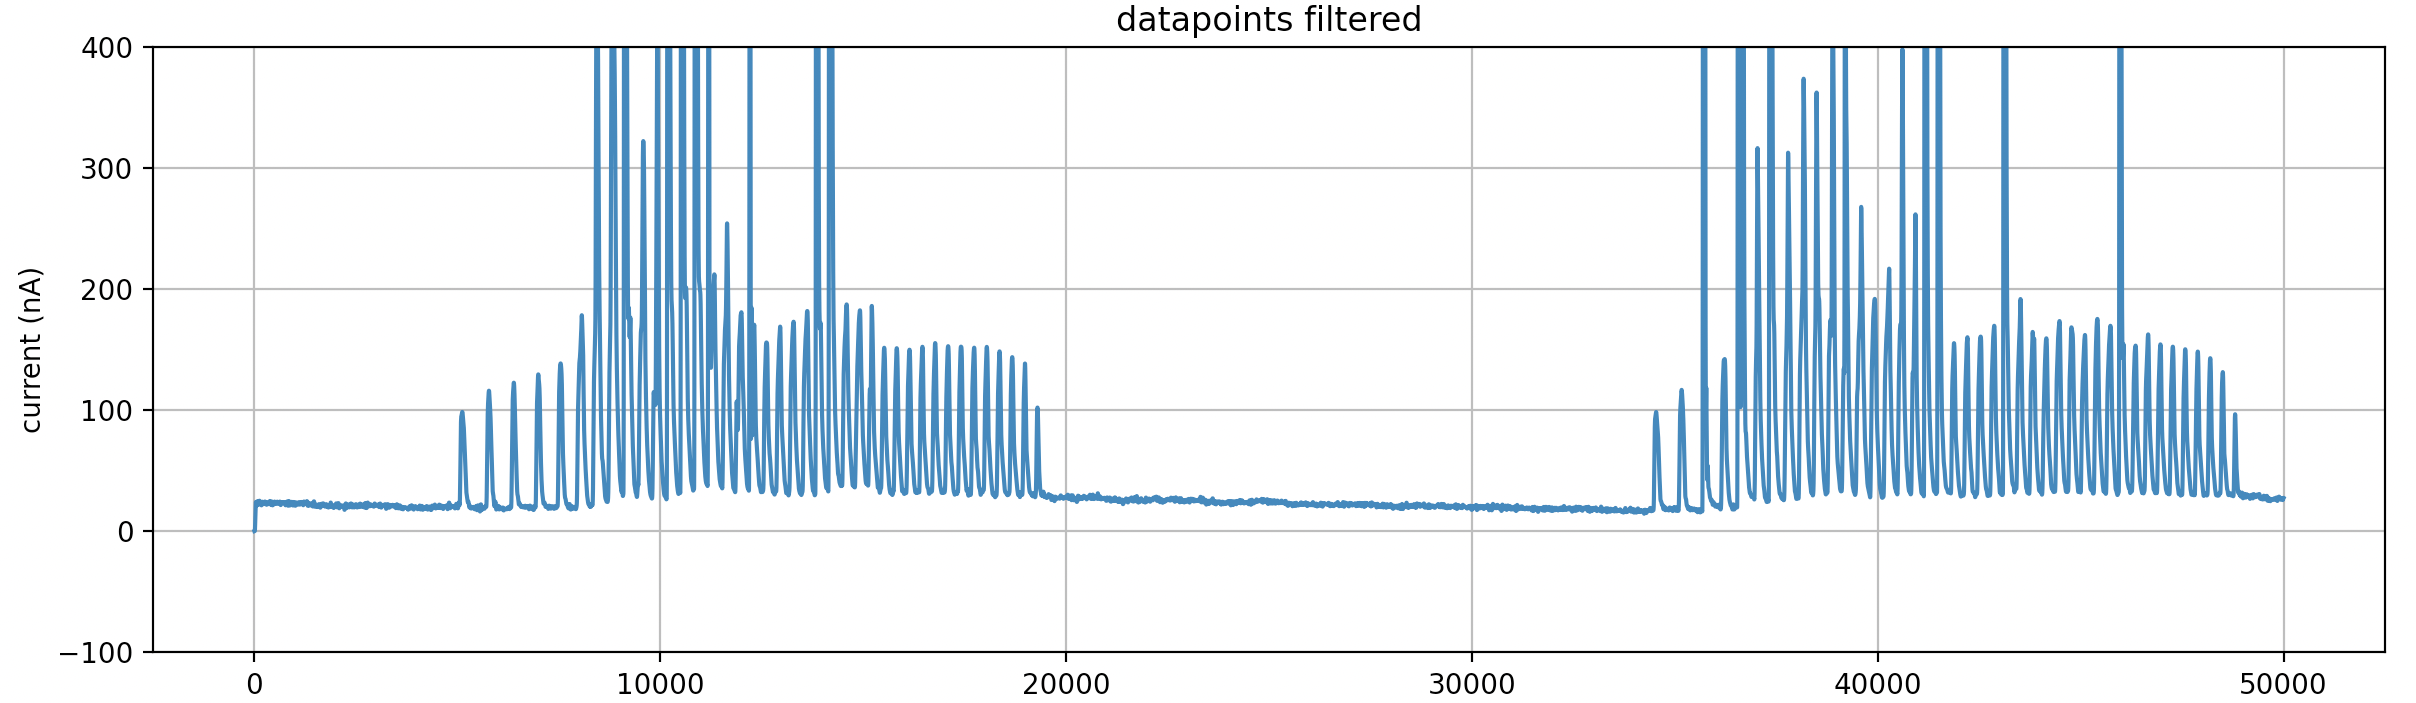
\includegraphics{Figuras/report2/img2.png}}
    \caption{Current measurement sample of a micro-dripping spraying mode. This graph represents 0.5s sample. The sampling frequency is 100kHz. Hence we have 50000 current values.}
    \label{fig:microdripping_current_pic}
  \end{figure}

  The existing signal contains valuable data not only about dripping but also other modes of spraying, thus it can serve as a non-visual classifier.
  This report draws significant inspiration from Sjaak's\cite{Sjaaks} work, which identifies distinct statistical characteristics of electrical current for various spraying modes.

\section{Scalling Laws}
\label{sec:scalling-laws}



\clearpage
\chapter[System Description]{System Description}
\label{chap:system_description}

In this chapter, we will discuss the equipment used in detail, including its integration and how it was modeled and implemented in both hardware and software. 
The python automation routine that is the focus of this project was started by a previous student\cite{Monica}, and the software itself was originally created as an electrospray multipurpose library \cite{Monica}.

\section{Hardware model}
\label{sec:hardware_model}

\subsection{Instrumentation}
\label{subsec:instrumentation}

The main instruments used for this project are listed below:

\begin{enumerate}[a)]

  \item High Voltage Power Supply (HVPS)
  
     - brand: FUG
    
     - model: HCP35-20kV
    
    The HVPS provides the electrical potential to the liquid, which can be applied by connecting the HVPS directly to the liquid feeding capillary or needle to a grounded electrode (usually a plate or a ring) located downstream.\cite{Monica}
    The setup has the USB serial interface for controlling and polling measurements.
    
    The software has an interface to integrate the HVPS to our routine. This interface can be found in \emph{FUG\_function.py} file where is located the functions used to control and collect data from this instrument.
    In case of change of equipment, a new interface must be created within this file to match another manufacturer specifications.

  \item Wireless Oscilloscope
  
     - Brand: \emph{TiePie engineering}

     - model: TiePie WifiScope WS6 DIFF
    
    The signal analysis with an oscilloscope using WiFi technology allows an in-depth case study of the electric current signal.
    The current is measured via a TiePie WifiScope WS6 from TiePie engineering that is a battery powered oscilloscope capable of transmitting data via a WiFi connection allowing it to be placed in the high voltage or ground path.
    
    Wireless communication allows us to make measurements disconnected to an external power supply, which gives us more safety when using high voltage potential references and also reduce the signal noise collected from external power lines.
    The current is routed directly via the input, hence the oscilloscope measures the voltage dropped via its input resistance (which can be switched between 1 or 2 Mohms).
    TiePie WifiScope WS6 has a resolution of up to 16 bit at a minimal input range of 200 mV, sufficient to measure currents down to 1 nA.

    The interface with the software was made using the TiePie Library\cite{TiePieLib} and can be found in \emph{configuration\_tiepie.py}. Note that is also important to have the \emph{printinfo.py} file in the project folder in order to work.

  \item Humidity and Temperature sensor
  
  The stability of the system is affected by many physical effects. Evidently having the more parameters analyzed favors the system control.
  The surface tension force is dependent of the liquid-gas interface on the meniscus. Hence, the surrounding gas must be constantly the same and so its humidity.
  Also, temperature is a variable that interfere in many phenomena in the system. Specially the liquid properties such as viscosity.

  For that, a standard microcontroller development board (\emph{Arduino Uno}) with a temperature and humidity sensor (DHT11) was configured to add that data in real time in the routine.
  The Arduino code can be found in the \emph{/peripherals} folder.
  

  \item High Speed Camera 
  
  - Brand: \emph{Photron}

  - model: Photron fastcam mini


  
  \item Syringe pump
  
  - Brand: \emph{Master dual}

  - model: WPI AL-1000

  The pump integration in the automation algorithm brings us a new controllable variable, the Flow rate. Now we can control the spraying mode with the
  two main variables that affect the system. 
  It will bring more complexity for the system since now we are dealing with multivariable control.
  Controlling also the flow rate gives to this project a new dimension in the system giving us freedom to explore the flow rate properties.
  With this new input variable our control is a MISO (Multiple Inputs Single Output) system.

  About the pump interface. As I could not find a good ready-to-use library for this pump I developed a simple and intuitive interface to be our software routine.
  The communication protocol used is RS-232. In the software routine the communication used is python serial interface. The pump commands list were found in the user manual.

  % The supply at constant pressure can also favor the stability of the spray\cite{prunet}. However, the flow rate depends on the applied pressure and pressure losses between the tank and the end of the capillary, which themselves are dependent on the liquid chosen and on its temperature. This volume flow rate may also depend on the applied voltage, since the electrostatic pressure on the meniscus produces a suction effect.

  \end{enumerate}


In figure \ref{fig:setup} we illustrate a diagram with all the key components of our system. The peripherals are connected to a computer running the software routine via serial communication. 
This diagram encapsulates our process system and will be used as a sub-system in our control model. The input of our process system are power supply voltage and pump machine flow rate, referred here as the controller values. The output is the oscilloscope current sample.

\begin{figure}[H]
  \centering
  \resizebox{150mm}{!}{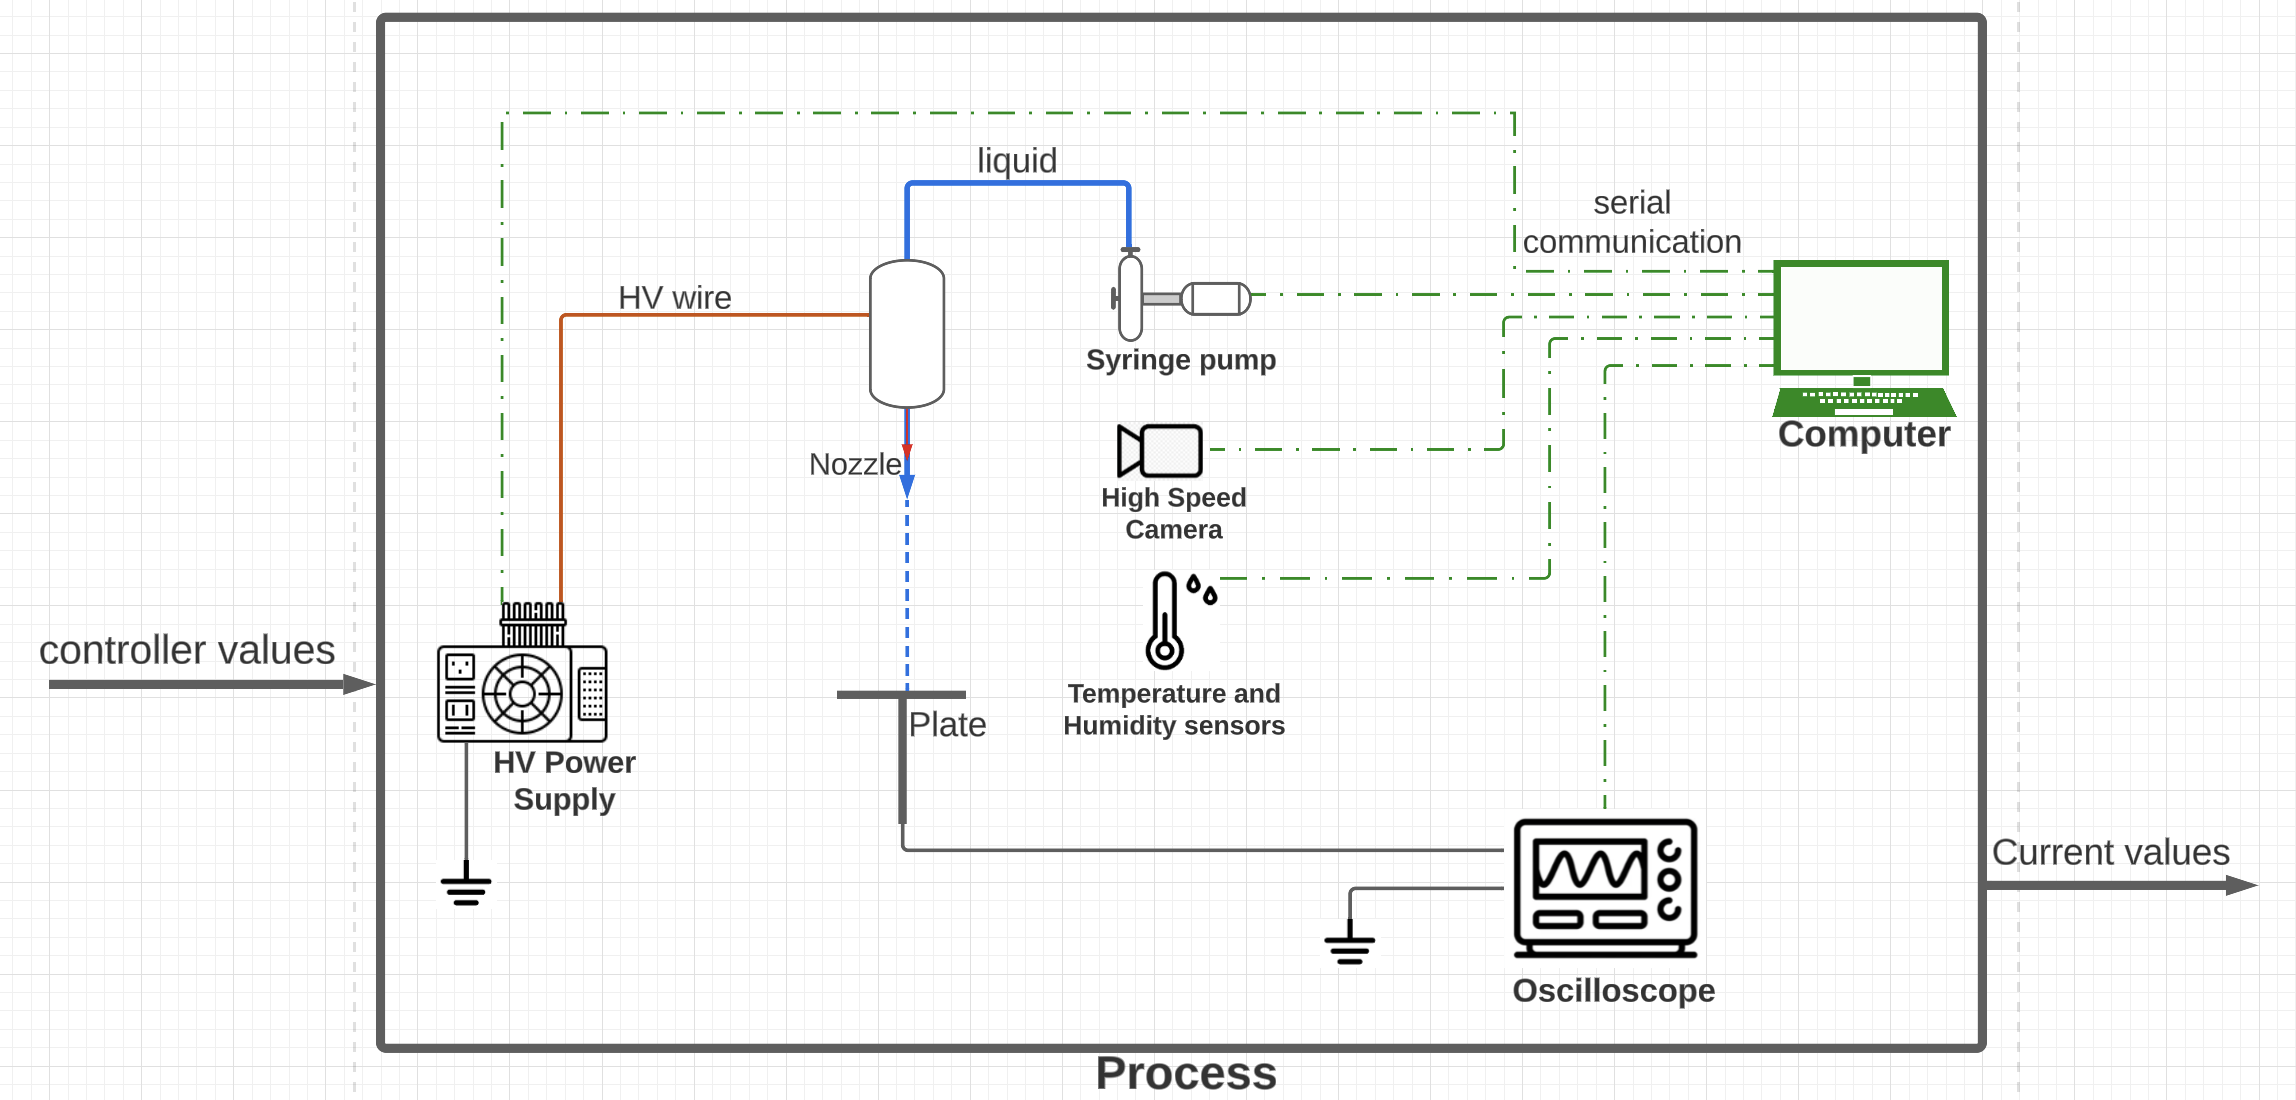
\includegraphics{Figuras/new_system_setup.png}}
  \caption{EHDA automation system setup}
  \label{fig:setup}
\end{figure}

There are also many minor variables that affects the experiment stability. More details are explained in \ref{sec:setup_validation}.


\section{Software Model}
\label{sec:control_model}

The software was reformulated on top of the control model represented in figure \ref{fig:control_model_fig}. The process of the control loop is the same as represented in \ref{fig:setup}. 
Each other subsystem in the control loop is a separate thread that will be explained bellow.

\begin{figure}[H]
  \centering
  \resizebox{150mm}{!}{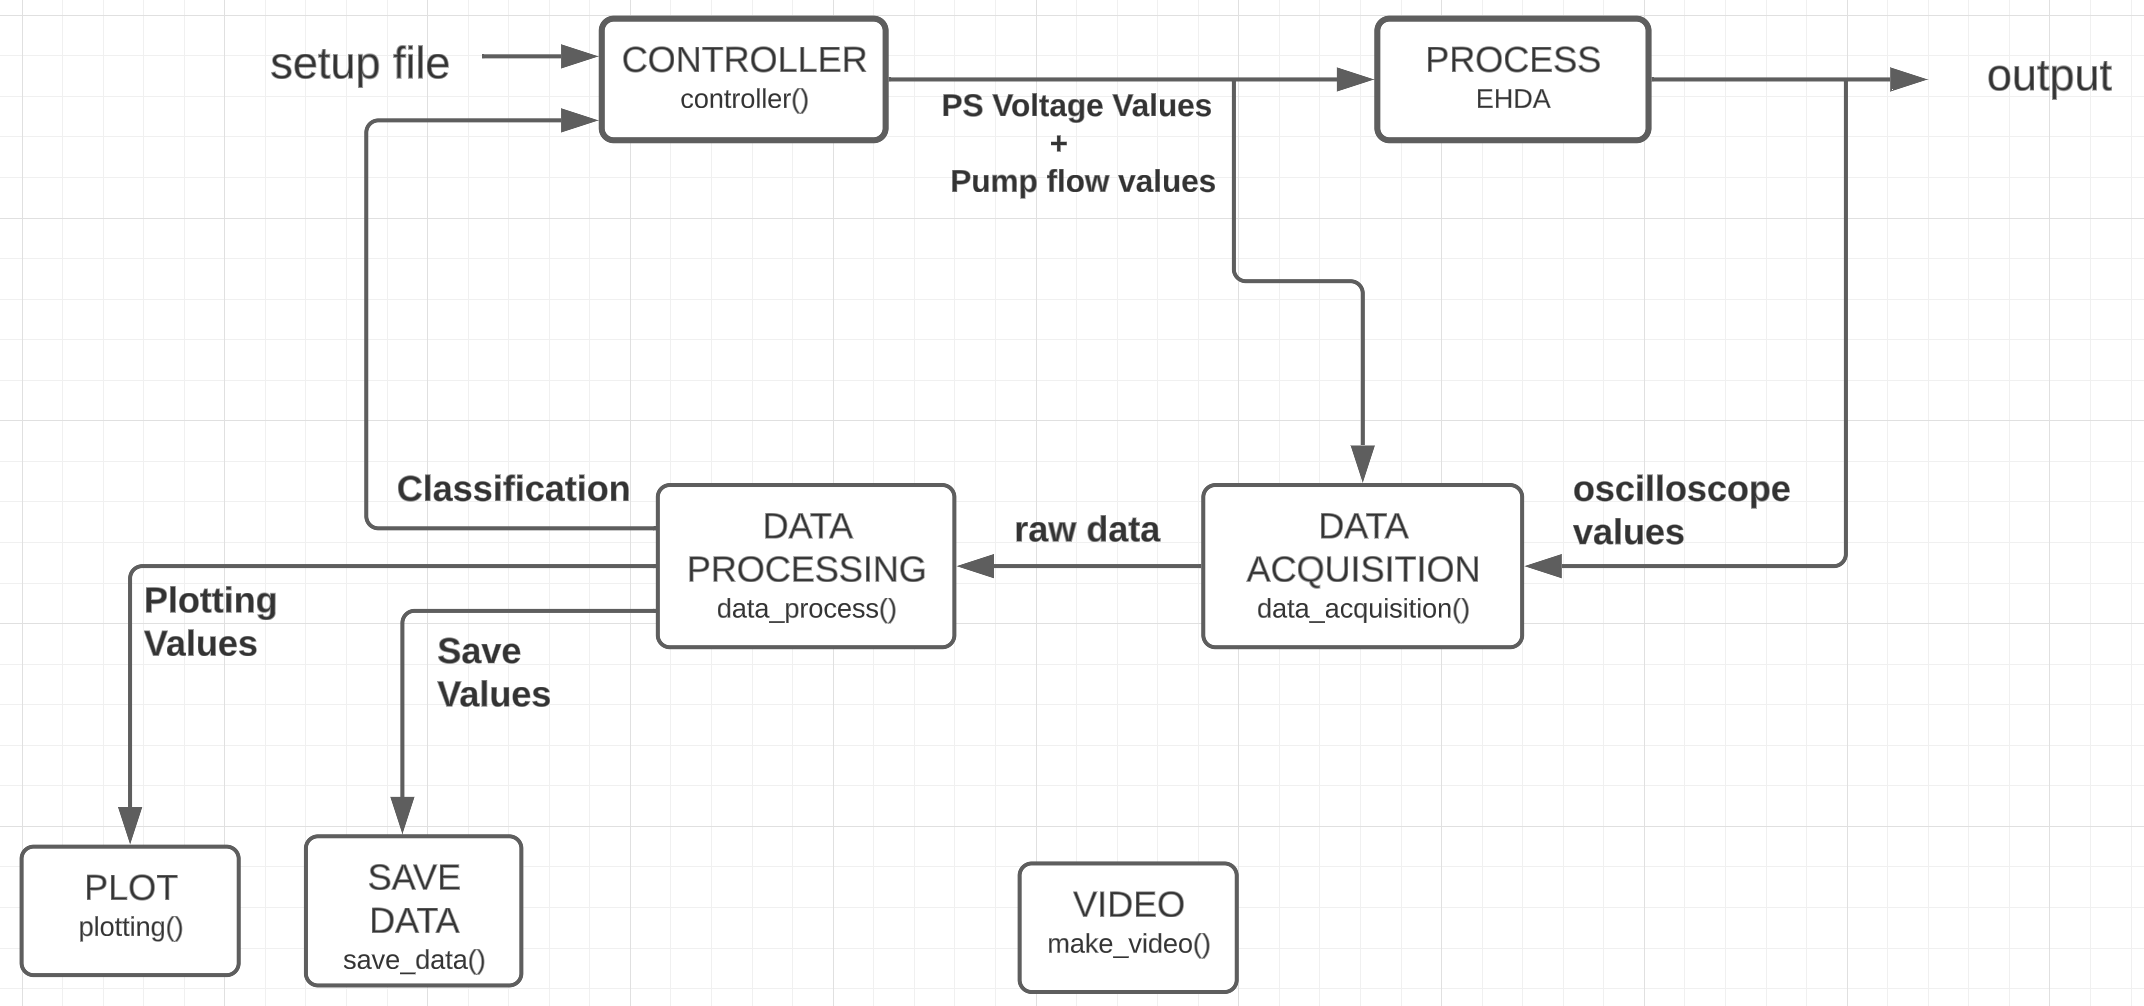
\includegraphics{Figuras/april/control_model.png}}
  \caption{EHDA automation system setup}
  \label{fig:control_model_fig}
\end{figure}

\subsection{Threading and Queues}
\label{subsec:concurrency}

    In order to implement this closed loop control model to the software and explore parallel processing, each sub-system was implemented as a separate Thread.
    For concurrency on flux of data between threads was used queues structures.
    A queue is an abstract data type that holds an ordered, linear sequence of items. You can describe it as a first in, first out (FIFO) structure.

    
    \subsection{Controller Thread}

        It is responsible for sending the power supply set voltage values and the syringe pump the flow rate set values according to the sequence selected.
        Also, responsible for sending the finish event command that end the routine and trigger the threads to close their routines.
        As input, we have the setup config file and the \emph{feedback\_queue}. As output, we have the values in the \emph{controller\_output\_queue()}.

    \subsection{Data Acquisition Thread}
    \label{subsec:data_aquisition}

        It is responsible for reading the current data from the oscilloscope, humidity and temperature data from the DHT11 sensor, voltage from the power supply, flow rate from the pump and concatenate into one sample data.
        As output, we have the values in the \emph{data\_queue()}.

    \subsection{Data Processing Thread}

        It is responsible for calculating the statistical values from the raw data and classify it in the respective spray mode for that sample.
        As output, we have the values in the \emph{save\_data\_queue()}, \emph{plotting\_queue()} and \emph{feedback\_queue()}.
    
    \subsection{Save Data Thread}
    \label{subsec:save_thread}

        After processing, the data is saved in real time in a json file using \emph{jsonstreams} library to save one sample structure at a time.
        With the new streaming model of saving a new structure of the collected data were created.
        Instead of having all data measurements values and after all data processing values we now are saving for each sample the measurements and processing values.
        The data acquired in each sample of 0.5s is shown in figure \ref{fig:data_sample}.
    
        \begin{figure}[H]
            \center
            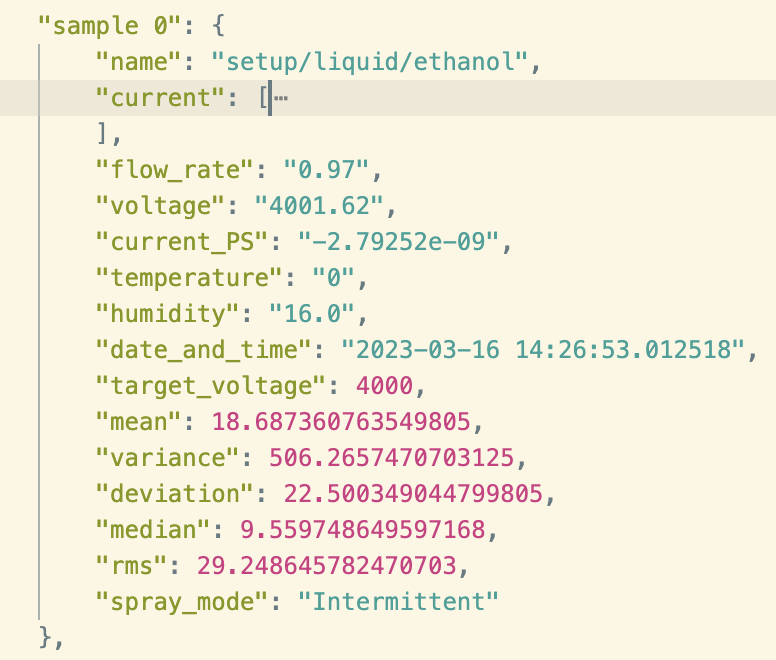
\includegraphics[width=10cm]{Figuras/19:03/new_sample.png}
            \caption{Output data json structure}
            \label{fig:data_sample}
        \end{figure}
    
        This new way of saving the measurement and processing data altogether separate by enumerated samples prevents loss of data in case of error during experiments and, specially improve in the usability of the data for further deep analysis. One experiment of around 1 hour collects around 6 GB of data. Organizing that amount of data to make it fast and easy to use was an important improvement in the software.
        To work and analyze the data we can use  pandas Data frame. A python widely used framework for data analysis.
        With the command:
        
        pandas.read\_json('PATH', orient='index').

        It will construct a Data frame with all data organized by samples.
    
        To conclude, json files are good as a system output because of its human readability. But as the database gets bigger json becomes to be a slow to read and heavy way to store the data. For that, saving the data frame in a compressed type of file called feather is much faster to work with the data.
    
    \subsection{Video Thread}

        Normally deactivated, that thread is responsible for triggering the camera in case we want to save a video of that sample.
    
    \subsection{Plot}

        The only running function that is not a thread because of the plotting library \emph{matplotlib} incompatibilities of running outside the main function. 
        It is responsible for plotting in real time the current sample acquired, and its respective fast Fourier transform to evaluate the sample frequency spectrum.
        It takes as input the \emph{plot\_data\_queue} from the \emph{processing\_thread()} and displays three graphs updated in real time on the screen during the experiment.

  \section{Chapter conclusion}

    In this chapter we described the system description detailing the hardware instruments, how it was modelled and its implementation in the software. Figure \ref{fig:Methodology_example1} shows a print screen of the user interface during an experiment.

    \begin{figure}[H]
      \centering
      \resizebox{150mm}{!}{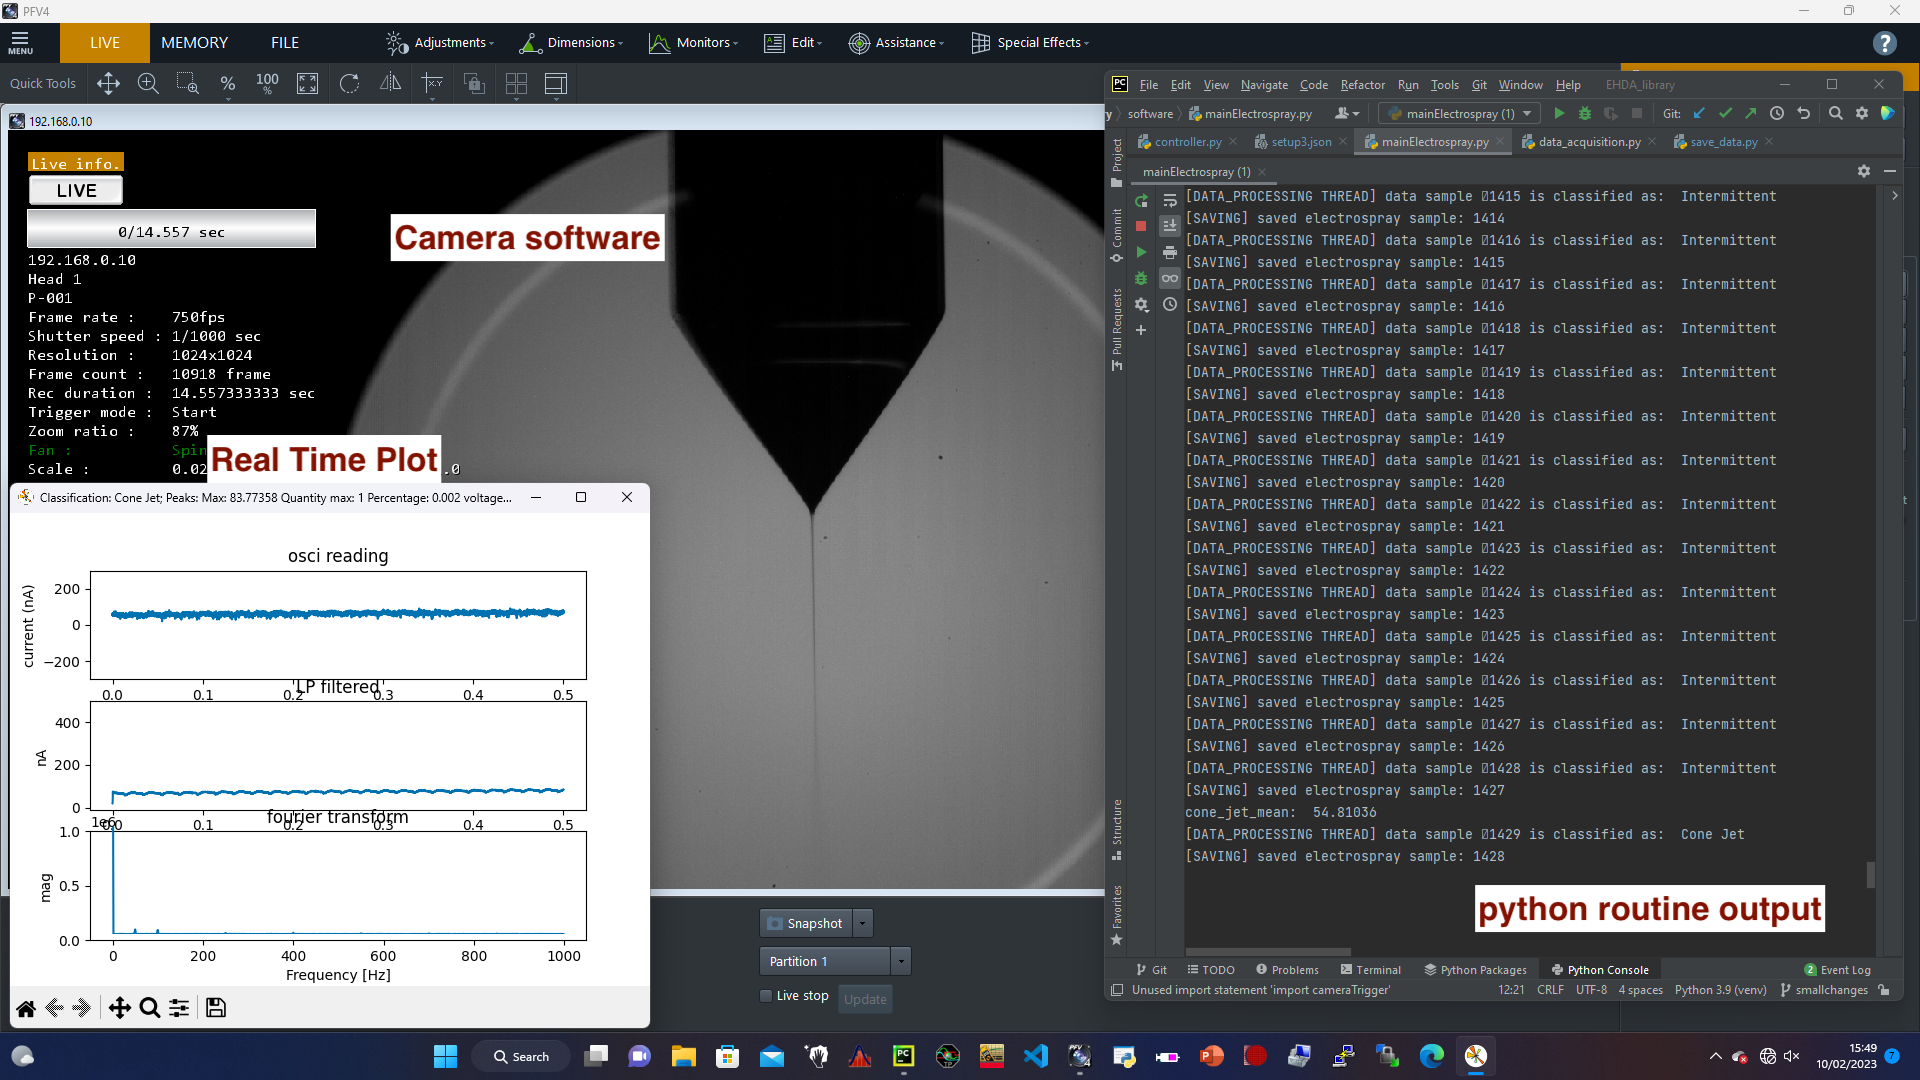
\includegraphics{Figuras/report4/experiment_print1.png}}
      \caption{EHDA automation system setup}
      \label{fig:Methodology_example1}
  \end{figure}
\clearpage

\chapter{Metodology}
\label{chap:Metodology}


\section{System Model}
\label{sec:control_model}

ilustramos o processo com a Figura \ref{fig:control_model_fig}. 

\begin{figure}[thpb]
  \centering
  \resizebox{150mm}{!}{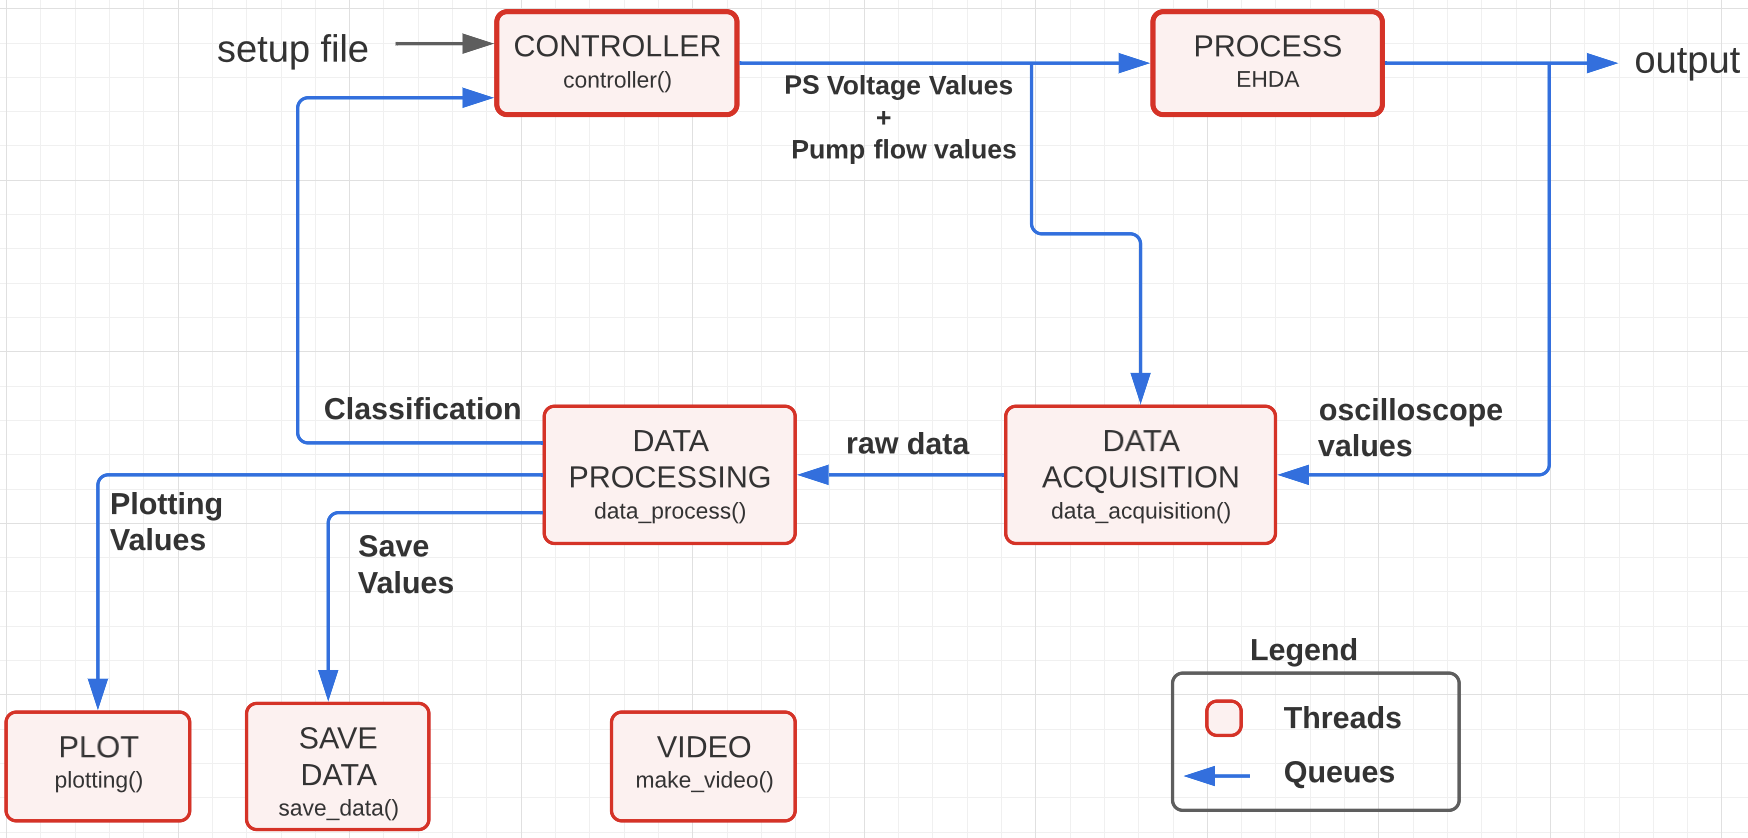
\includegraphics{Figuras/control_loop.png}}
  \caption{EHDA automation system setup}
  \label{fig:control_model_fig}
\end{figure}

\section{Threading and Queues}
\label{sec:concurrency}

    In order to implement this system model to the software and explore parallel processing each system in the
    model was developed as a separate Thread. For cuncurrency purpose and the flux of data in the control cicle was used queues structures.
    
    \begin{enumerate}[a)]
        \item Item 1;
        \item Item 2; 
        \item Etc.     
    \end{enumerate}

\section{Classification}
\label{sec:section_classification}

\subsection{Statistical Analisys}

 According to \cite{Sjaaks} evaluating the current data flowing through the nozzle to the plate we can analyze the signa that represents the spraying dynamics.
 through statistical analysis in this signal such as mean value and standart deviation we can analyze if the signal is stable or not.

 Our classification by statistical analysis was implemented in the automation library made by the previous student \cite{Monica}.

 Each current sample is 0.5s of current data in 10kHz sampling frequency.
 By the processing thread we take this sample and evaluate the followings statistical values.
        
        - Sjaak Classification -> Classifies Dripping, Intermittent and Cone Jet
        
        - Monica Classification -> Classifies Corona Sparks

        - João Classification -> Classifies Multi Jet

	The algorithm implemented works in the following way:
	\begin{algorithm}
        \caption{Statistical Classification}\label{alg:statistical_class}
        \begin{algorithmic}
        \Function{statistical\_classification}{$sample$} 

            \State $spray\_mode \gets "Undefined"$;
            \State $mean \gets sample.mean$; 
            \State $std\_deviation \gets sample.std\_deviation$;
            \State $median \gets sample.median$;
            
            \If{ $mean / std\_deviation$ > 2.5}
                \Comment{Sjaak classification \cite{Sjaaks}} 
                \State $spray\_mode \gets "Dripping"$;
            \ElsIf{$ 2.5 < mean / std\_deviation < 2.5 \And mean / std\_deviation > 0.3 $}
                \State $spray\_ mode \gets "Intermittent"$;
            \ElsIf{ $mean / std\_deviation$ < 0.3}
                \State $spray\_ mode \gets "Cone Jet"$;
                \State $cone\_jet\_mean \gets mean$;
            \EndIf

            \If{ $mean / std\_deviation$ > 2.5}
                \Comment{Monica classification \cite{Monica}} 
            \EndIf

            \If{ $spray\_mode == "Cone Jet"$}
                \Comment{João classification} 
                \If{ $cone\_jet\_mean > 1.14 \times mean$}
                    \State $spray\_ mode \gets "Multi Jet"$;
                \EndIf
            \EndIf

            \Return $spray\_ mode$;
        \EndFunction
        \end{algorithmic}
    \end{algorithm}


\subsection{Machine Learning}


\section{Routine Sequences}
\label{sec:routine_sequences}

    The software was previously developed as a electrospray multipurpose library\cite{Monica}. 
    Continuing this methodology, in the setup json file there is a "sequence" atribute which can chosen beetween "ramp", "step", "map" or "control".
    The controller thread will manage what the algorithm must do for each sequence.

\subsection{Ramp}



\subsection{Step}


\begin{algorithm}
    \caption{STEP sequence in controller thread}\label{alg:stepping_algorithm}
    \begin{algorithmic}
    \Procedure{STEP}{$voltage\_start,voltage\_stop$} 
        \State $voltage \gets voltage\_start$
        \While{$voltage \leq voltage\_stop$} \Comment{scanning voltage range}
            \State \Call{send\_voltage\_command}{voltage}
            \State \Call{sleep}{step \_time}
            \State $voltage \gets voltage + step\_size$
        \EndWhile
    \EndProcedure

    \end{algorithmic}
\end{algorithm}

\subsection{Map}

    \begin{figure}[H]
        \center
        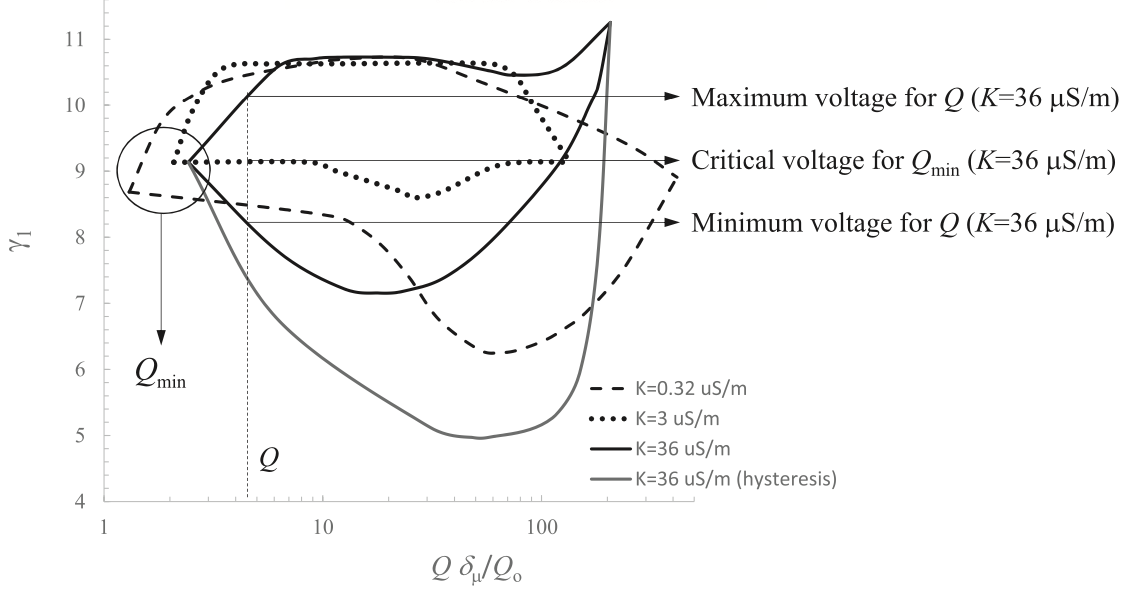
\includegraphics[width=13cm]{Figuras/ganan_calvo_map.png}
        \caption{Domains of existence (stability) of Taylor cone-jets. \cite{gananCalvo} }
        \label{fig:ganan_calvo_fig}
    \end{figure}


    \begin{algorithm}
        \caption{MAP sequence in controller thread}\label{alg:mapping_algorithm}
        \begin{algorithmic}
        \Procedure{MAP}{$flowrate\_values$} 
            \ForAll{flowrate\_values}  \Comment{scanning in the flowrate range}
                \State \Call{send\_flowrate\_command}{flowrate}
                \State $voltage \gets voltage\_start$
                \While{$voltage \leq voltage\_stop$} \Comment{scanning in the voltage range}
                    \State \Call{send\_voltage\_command}{voltage}
                    \State \Call{sleep}{step \_time}
                    \State $voltage \gets voltage + step\_size$
                \EndWhile
            \EndFor
        \EndProcedure

        \end{algorithmic}
    \end{algorithm}

    In the figures 5 and 6 we can see the results of this mapping experiments. The liquid used is pure ethanol. 
    Each figure has 3 graphs with shared x axis representing the samples collected. The first is the current values collected through all the experiment.
    The second is the voltage values applied in each window of data collected. The colors represent the spraying classification defined by our routine.
    The third graph shows the current mean value of each data sample.
    Note that the experiment is composed of loops that increase voltage, change flowrate and repeat.


    \begin{figure}[H]
        \center
        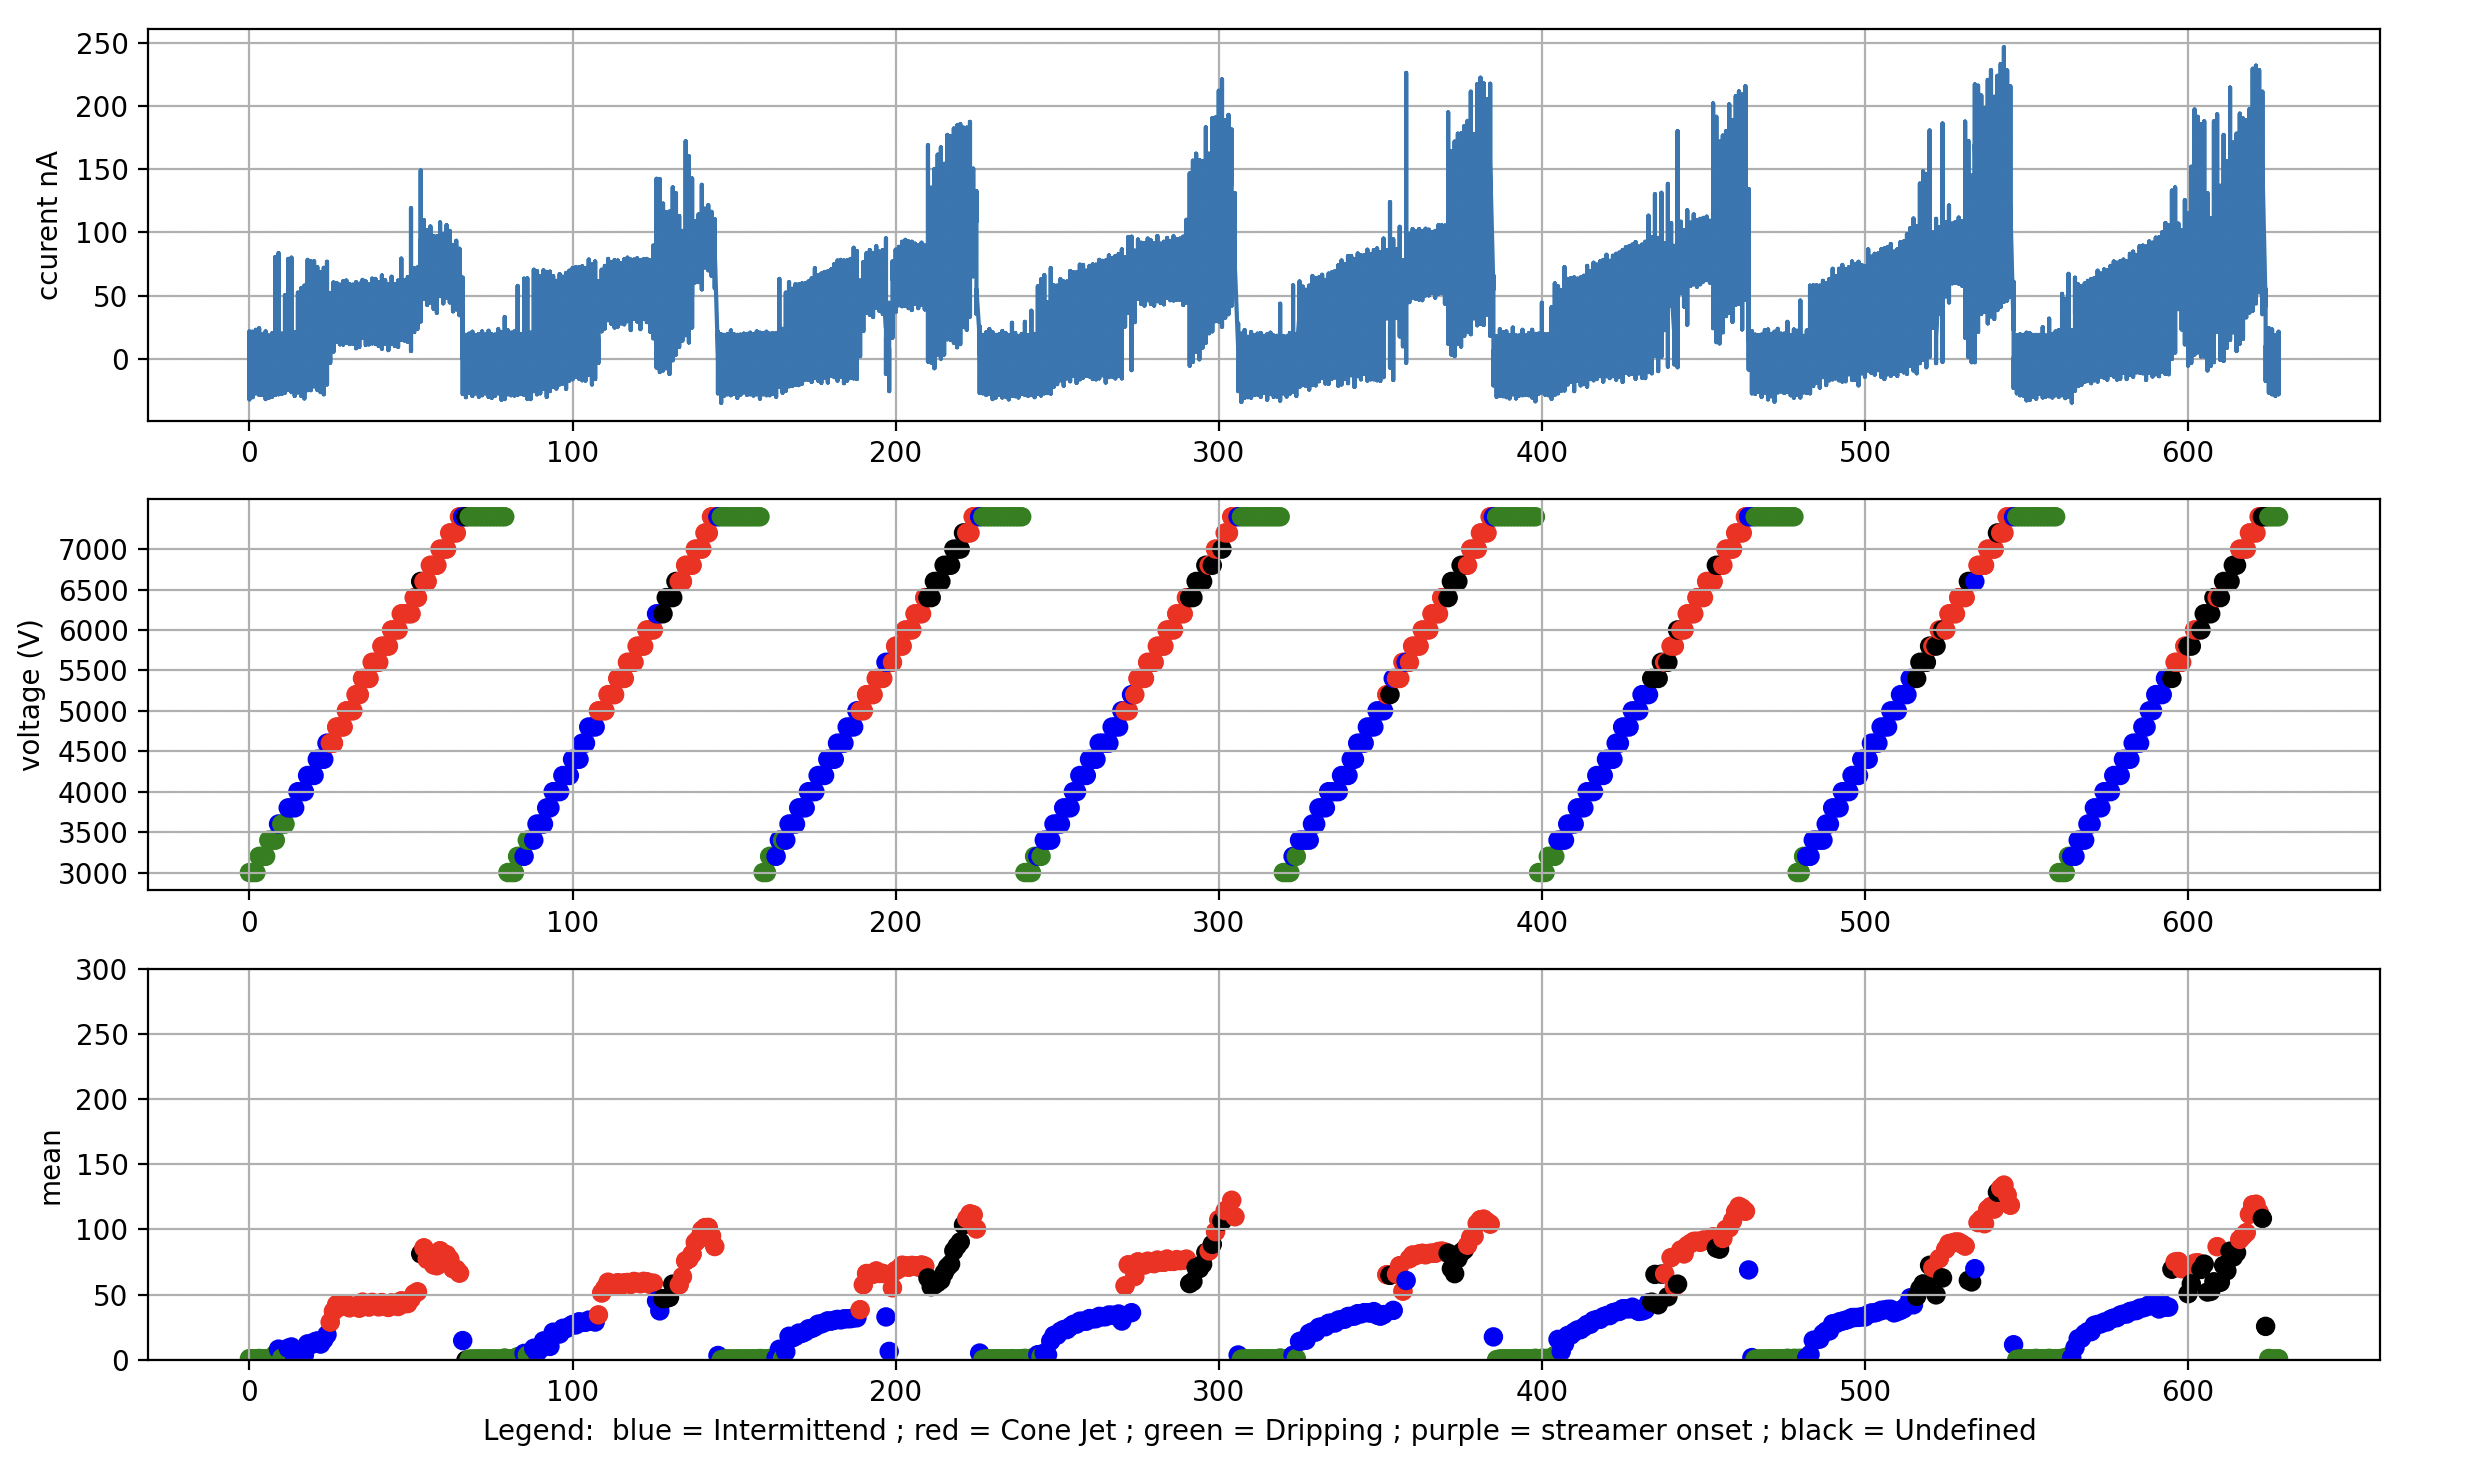
\includegraphics[width=15cm]{Figuras/report2/map2Data.png}
        \caption{Mapping Experiment example 1}
        \label{fig:map2Data_fig}
    \end{figure}


    \begin{figure}[H]
        \center
        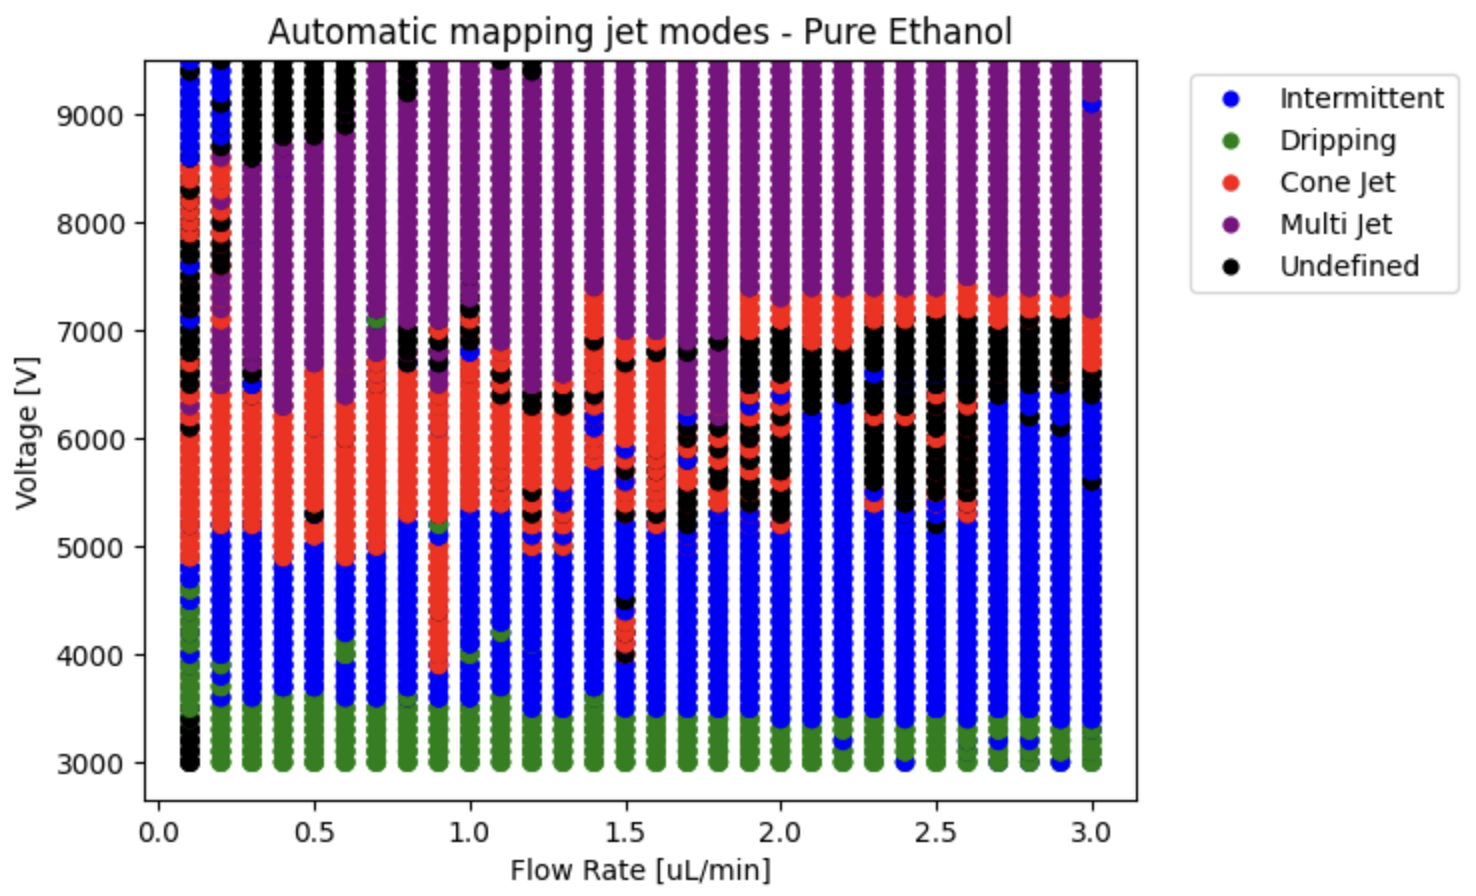
\includegraphics[width=15cm]{Figuras/report4/map-2023-03-02.png}
        \caption{Mapping Experiment example 1}
        \label{fig:map3Data_fig}
    \end{figure}



\subsection{Control}

\section{Optimizations}
\label{sec:routine_optimization}

About the python algorithm to turn the experiment autonomous it was made a study and modelling of the software architecture to optimize it for further control loop application to be implemented. From the changes made until now it highlights:

- Integrate high speed camera to the experiment routine.

- Remodel the software to support threads in order to separate the sensoring and controlling routines.

- Reduce the data collected size.

- Synchronize the power supply step commands and voltage sensoring.

- Reestructure the setup file in order to make it more intuitive to use the experiment.

- Improvements in code organization and readability.

About the setup,integrate was changed the liquid, nozzle diameter and distance to the plate in order to
make the experiment the most stable and easy to reach cone-jet mode as possible. For example, while doing experiments we discovered that the frequency of the pump machine internal motors was creating an interference in the flowrate. Therefore compromising the stabilization in cone jet mode. A solution for that was to increasethe flowrate wich smooths this pumping noise. For that was also necessary to increase the nozzle diameter to balance with all other variables from the experiment.

\subsection{Pump Integration}

    The pump integration in the automation algorithm bring us a new controllable variable, the Flowrate. Now we can control the spraying mode with the
    two main variables that afect the system. 
    It will bring more complexity for the system since now we are dealing with multivariable control.
    Controlling also the flowrate gives to this project a new dimension in the system giving us freedom to explore the flowrate properties.
    % Our control model is now a MISO \footcite{MISO: Multiple Inputs Single Output} system. The crossover (couple) between the controlled variables will be evaluated in further reports.

    About the pump interface. As I could not find a good ready-to-use library for this pump I developed an simple and intuitive interface to be our software routine.
    The communication protocol used is RS-232. In the software routine the communication used is python serial interface. The pump commands list were found in the user manual.



\clearpage
\chapter{Results}
\label{chap:Results}

In this chapter, we will present the results obtained from our project. Firstly, we will demonstrate how the automation routine enhanced the research experiments. Next, we will discuss the validation of the classification results. Finally, we will showcase the performance of the implemented controller algorithms.

\section{Automation routine}
\label{sec:automation_routine}

The automated experiment routine is capable of acquiring a significantly more precise and extensive amount of data than what can be achieved by a human. Most power supplies available in the market rely on manual potentiometer adjustment to select the set point, which results in imprecise potential selection by a person. Moreover, manual adjustment takes some time to achieve the desired voltage. By running a computer routine that automatically sends commands to the power supply, we can achieve faster and more reliable experiment data.
We can see in figures \ref{fig:multi_class_exp1} and \ref{fig:multi_class_exp} the visual interface that the operator have during an experiment. All the important data of EHDA experiments are showed in the same screen and referring to each 0.5 seconds sampling time.

\begin{figure}[H]
    \center
    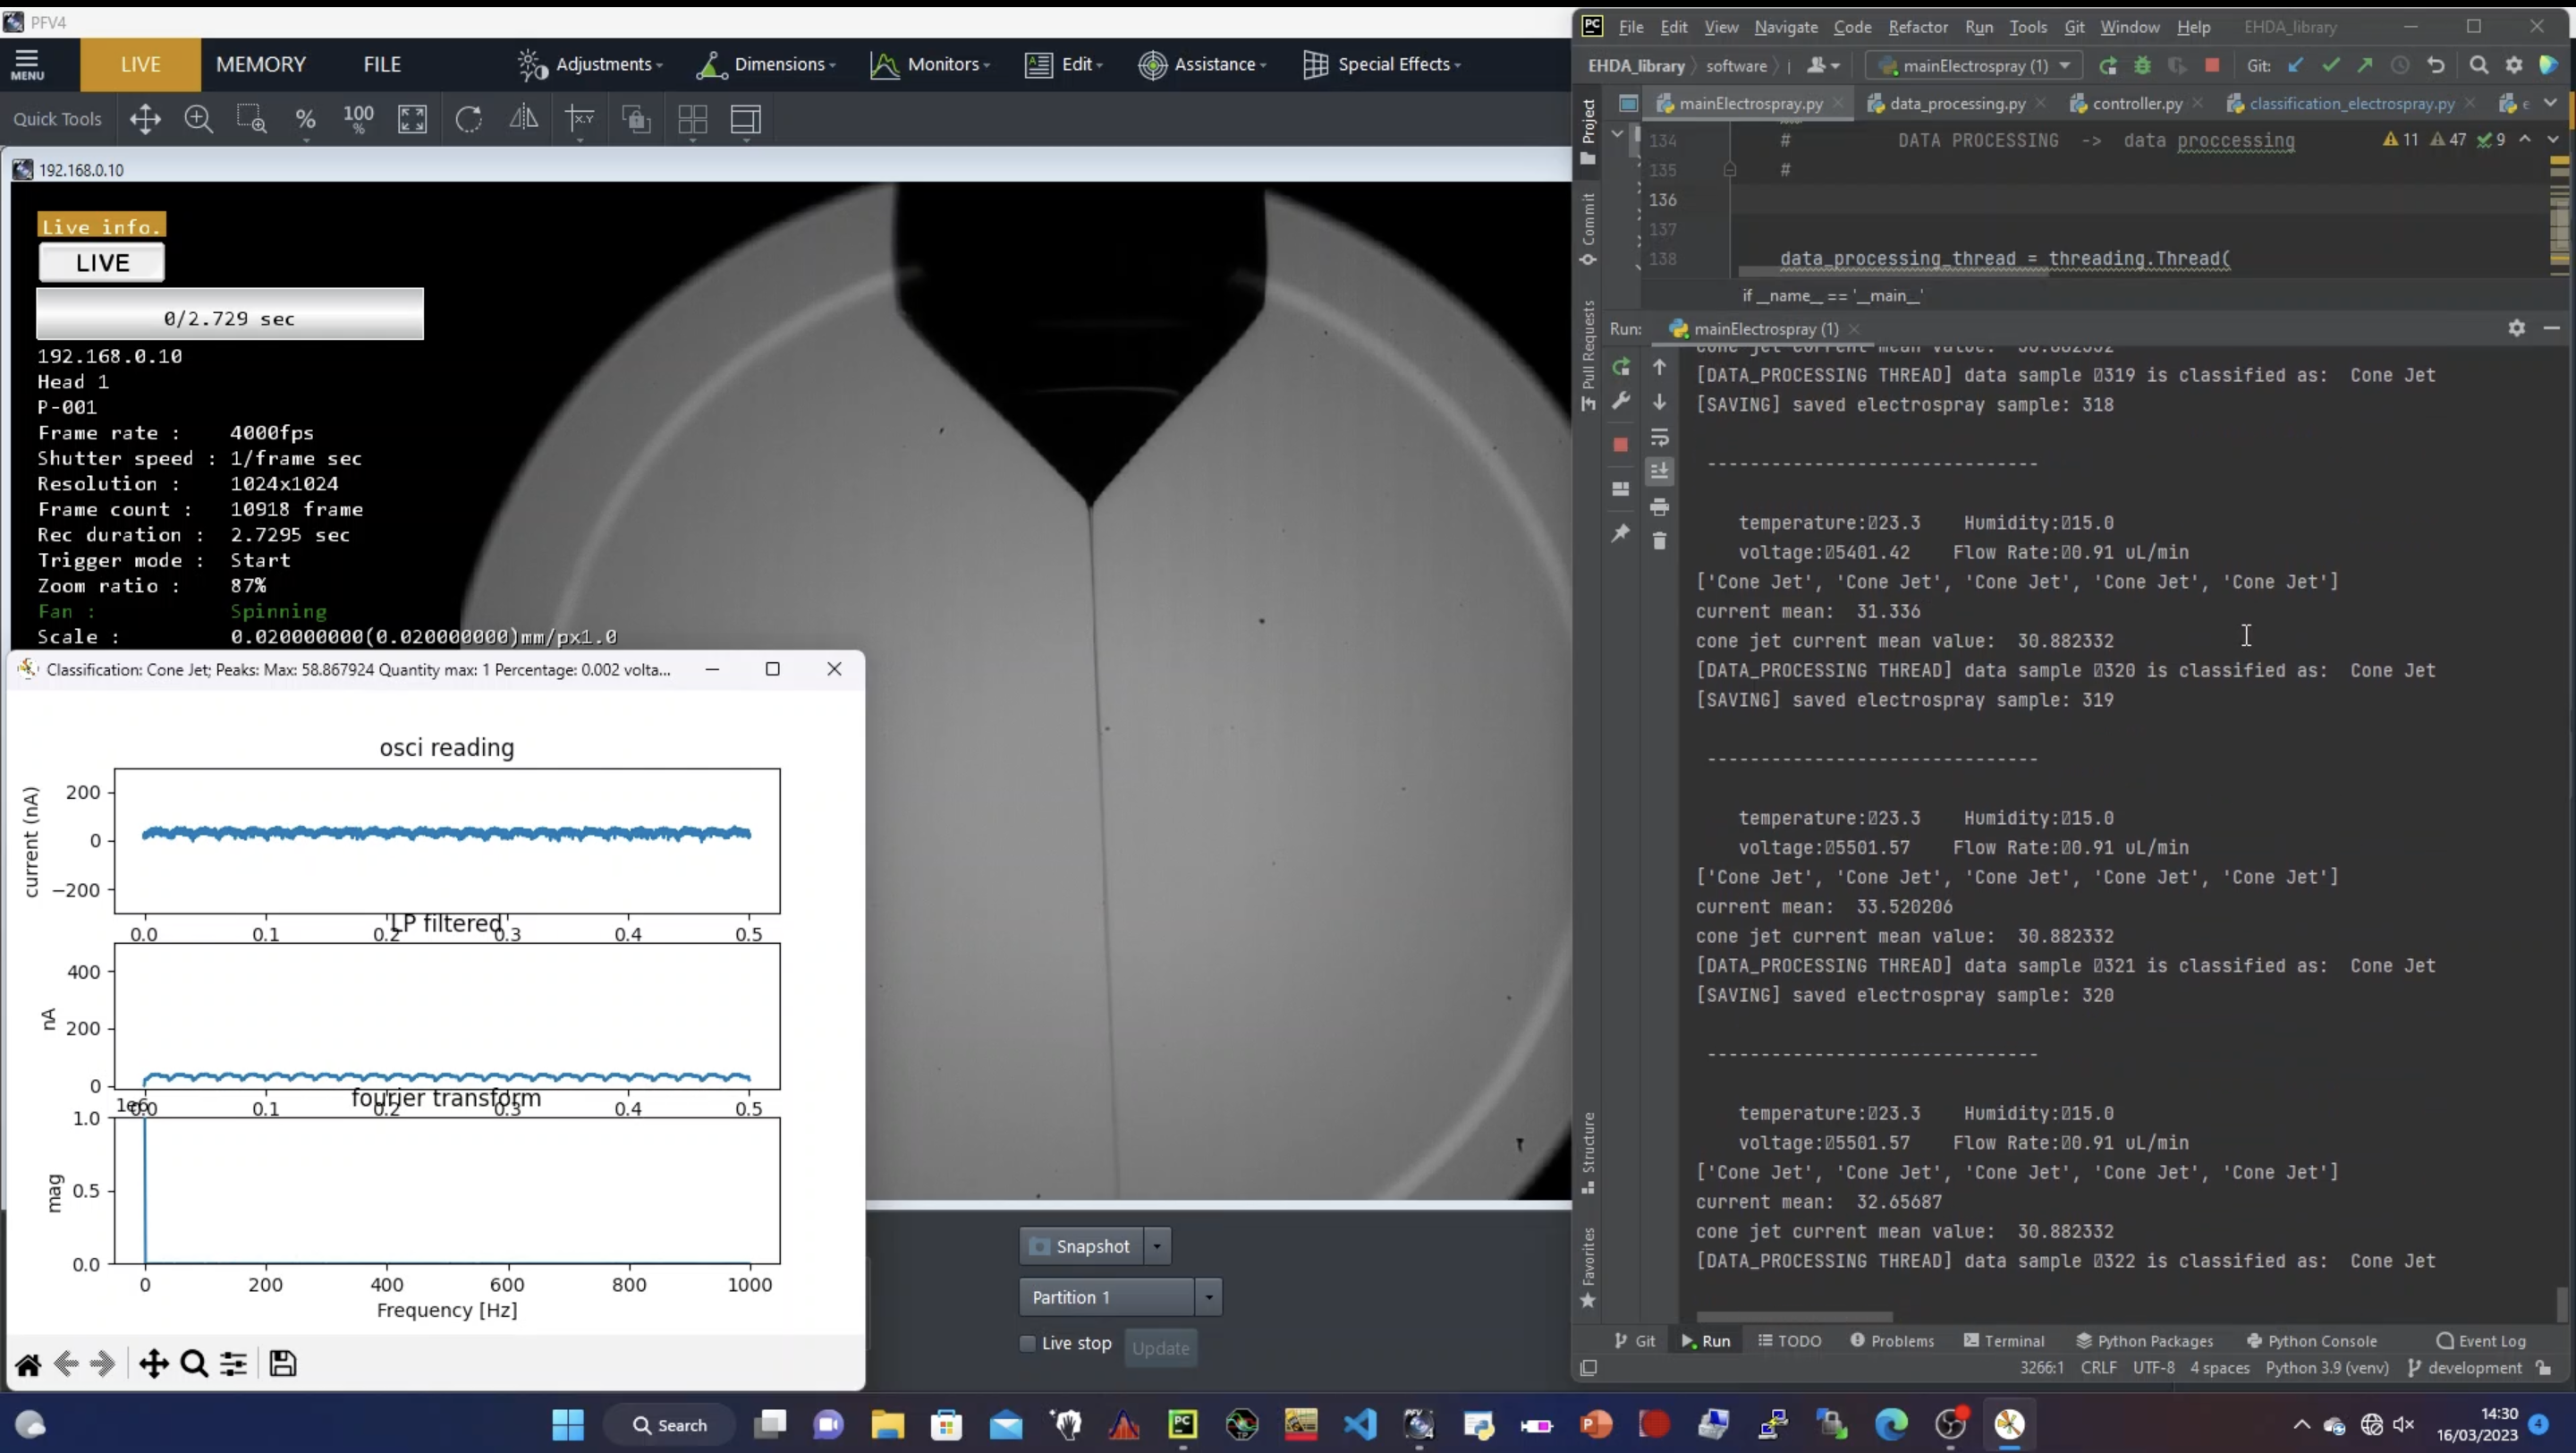
\includegraphics[width=17cm]{Figuras/19:03/axs1.png}
    \caption{Print screen of the window shows user interface during the experiment.
        We can see the image generated by the camera in the background.
        The routine code running in pycharm software on the right side.
        And also real time signal plottings of the current data on the left side.}
        \label{fig:multi_class_exp1}
\end{figure}


\begin{figure}[H]
    \center
    {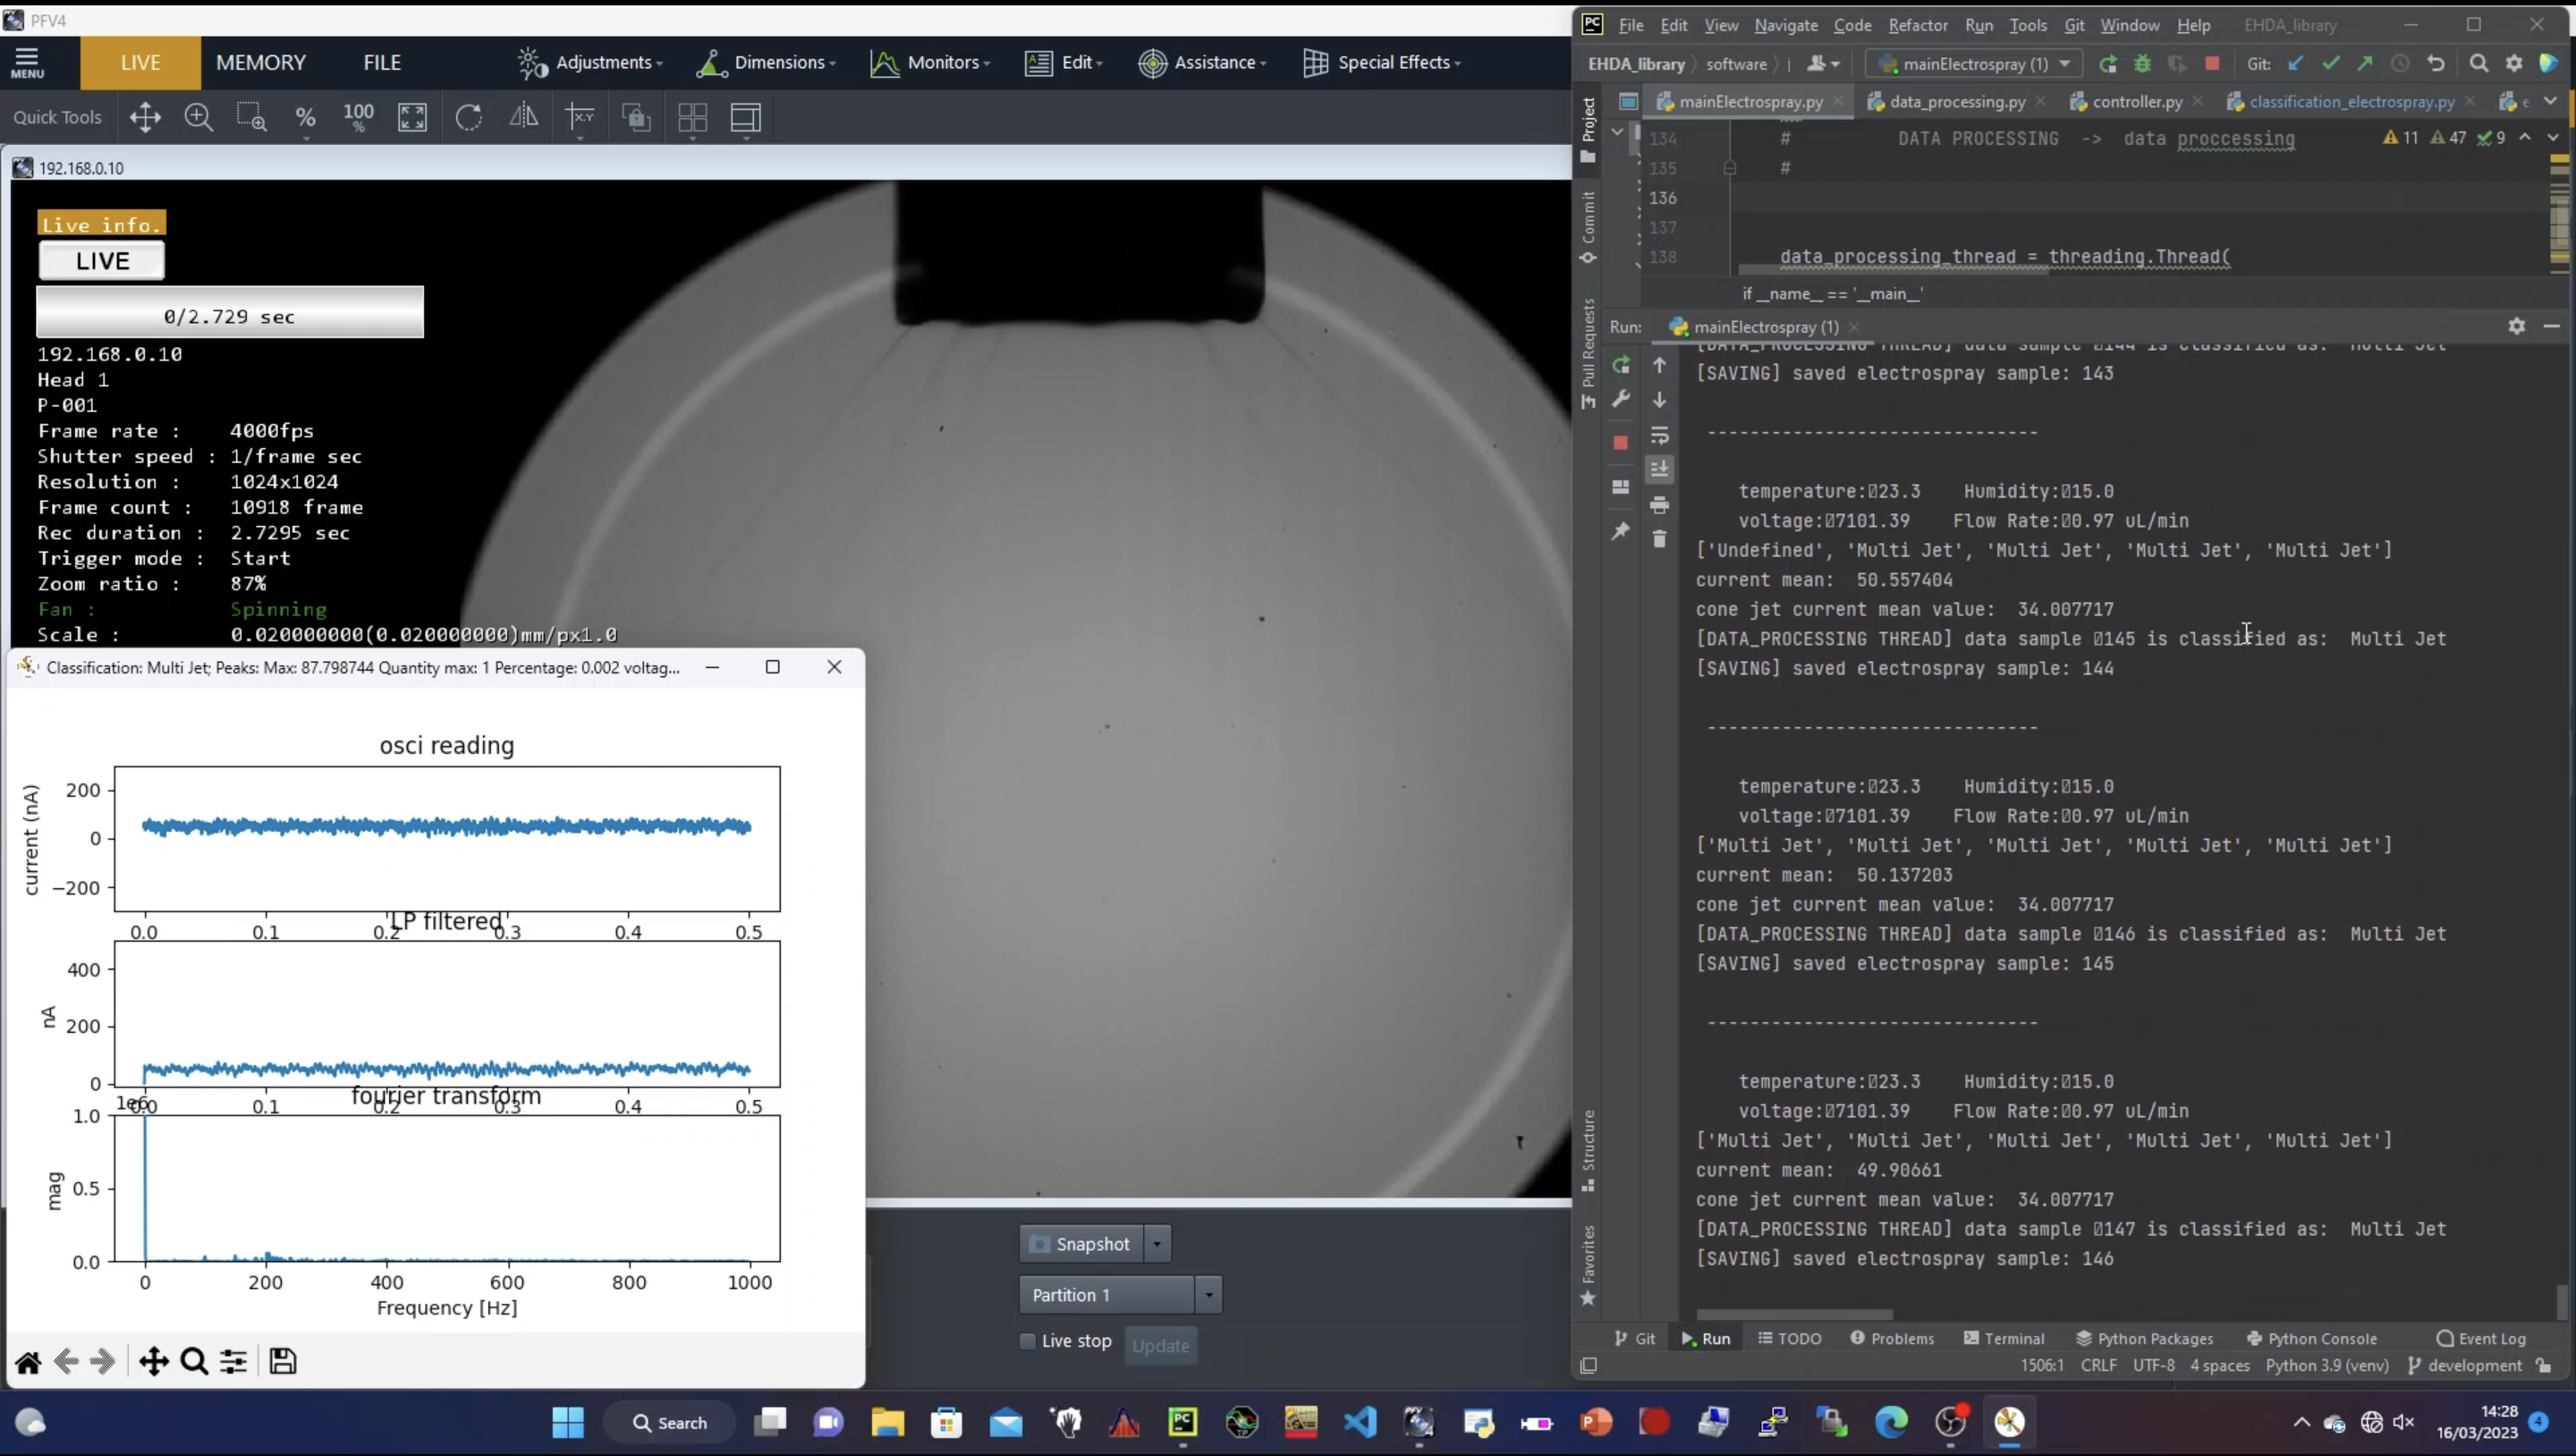
\includegraphics[width=17cm]{Figuras/19:03/axs2.png}}
    \caption{Print screen during an experiment. At this moment we are in Multi Jet spraying mode. At the left we can see the current signal has a smooth and constant curve. We can also see the automatic classification on the right side.}
    \label{fig:multi_class_exp}
\end{figure}


\section{Classification}
\label{sec:classification_results}

The results of the classification process were favorable for experiment automation, however, they may not be as effective for optimal performance of the controller.
The inaccuracy of the classification by statistical method in addition with the amount of variables that need to be syntonized for stabilize in cone jet or multi jet makes difficult the controller development.

\subsection{Step Sequence}
\label{subsec:step_results}

Our first classification results were made exploring just the voltage ranges. For that we tried to stabilize all the other parameters such as humidity, temperature and external noise.
First, we fixed a flow rate to 0.7 uL/min. and ran a step routine as defined in \ref{subsec:step_routine}. The figure \ref{fig:step_voltage} shows the step voltages during the experiment and figure \ref{fig:raw_data} illustrates the raw data acquired with it. In figure \ref{fig:class_step_data} we see the same experiment data classified by spraying mode and separated by color.


\begin{figure}[H]
    \center
    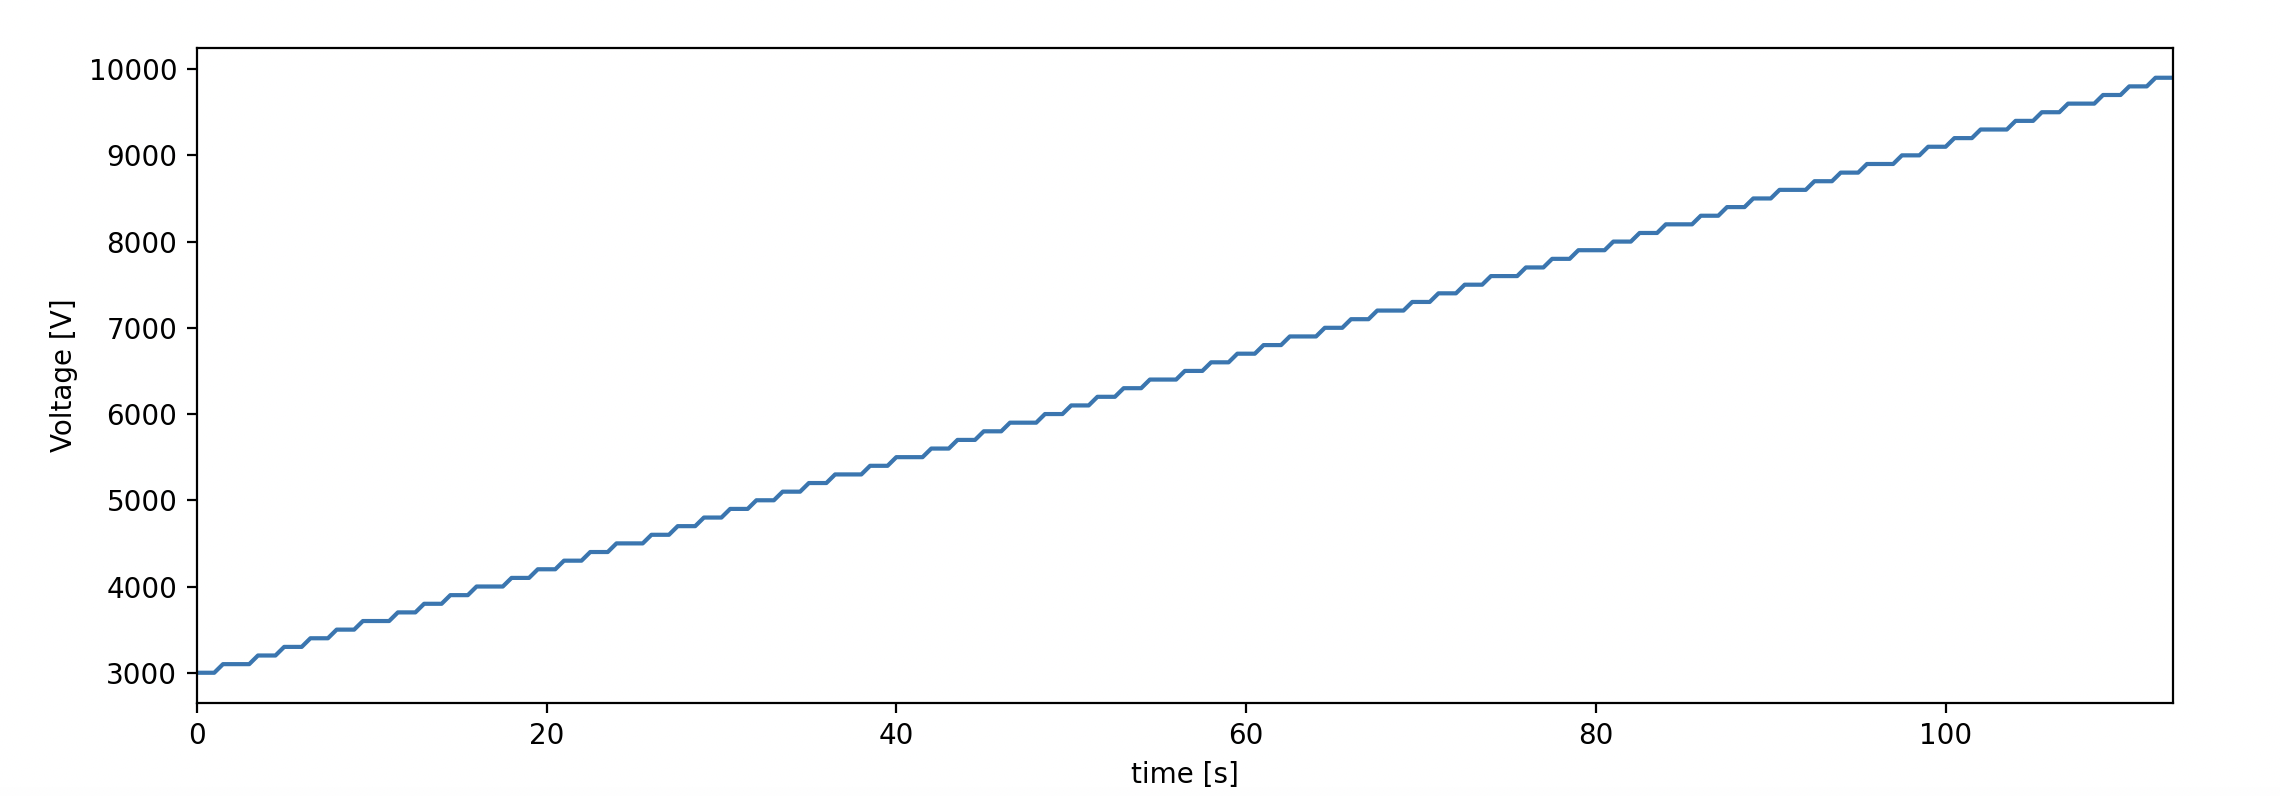
\includegraphics[width=12cm]{Figuras/19:03/voltage_step.png}
    \caption{Input voltage step graph. The range is between 3K-10K Volts. Step size of 50V and step time of 5 seconds.}
    \label{fig:step_voltage}
\end{figure}


\begin{figure}[H]
    \center
    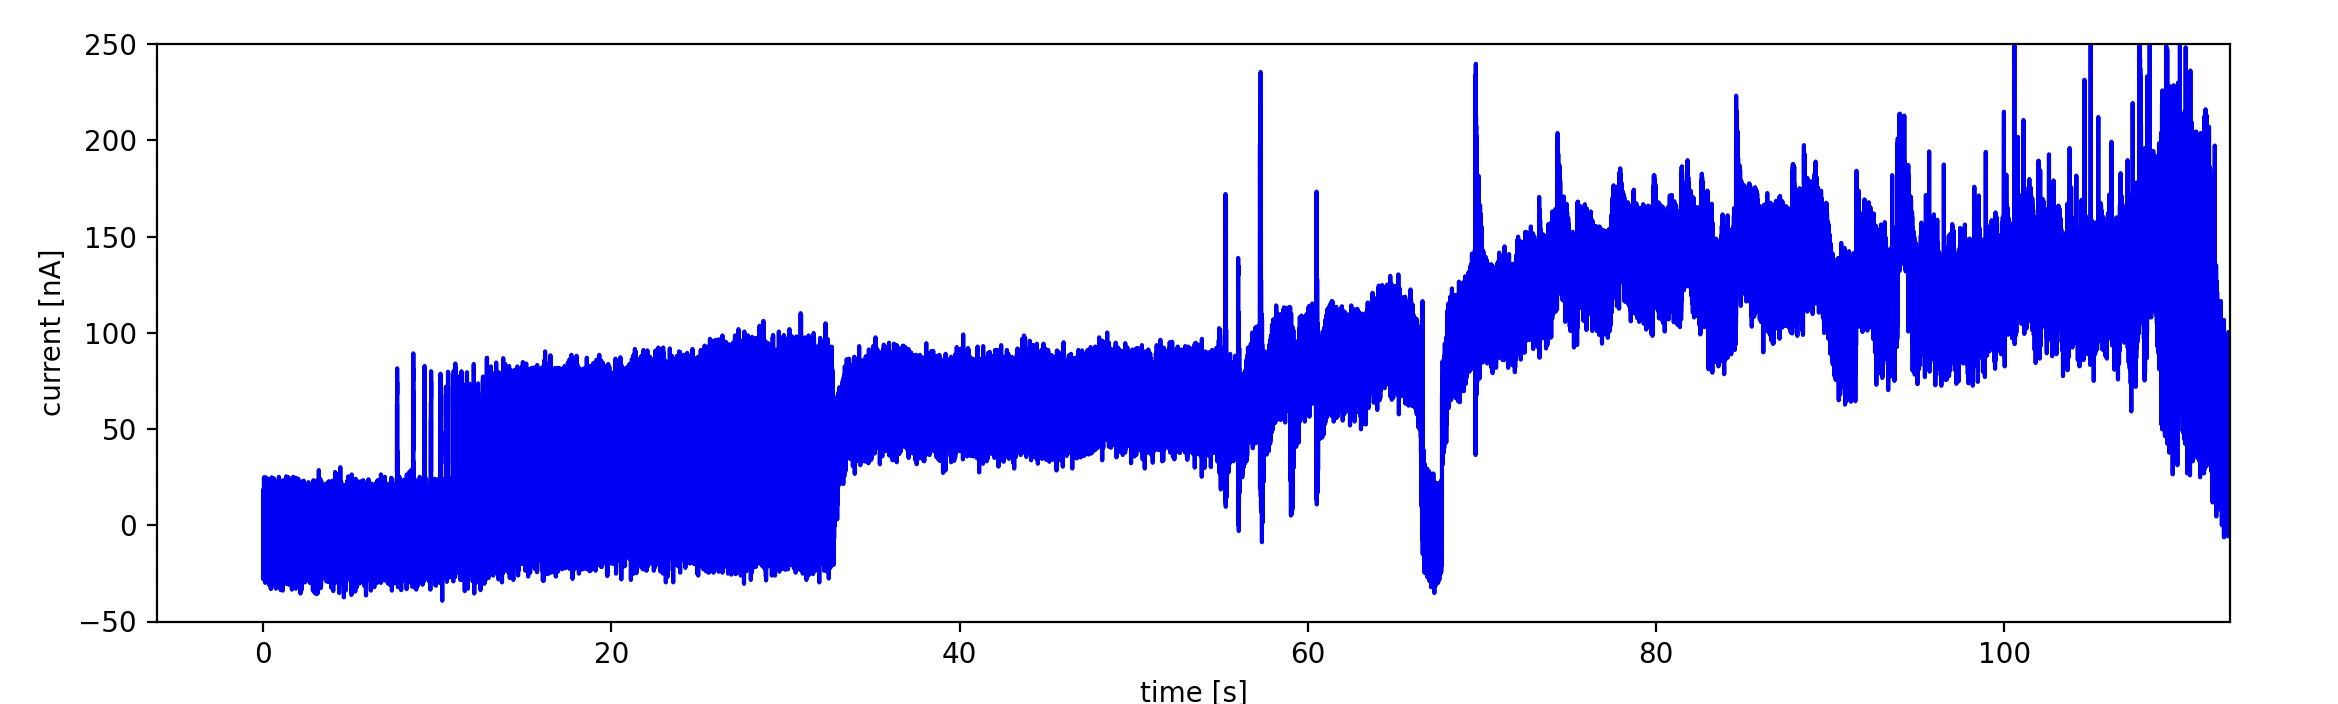
\includegraphics[width=12cm]{Figuras/19:03/raw-data-example.png}
    \caption{Output raw data collected in the voltage range experiment showed in \ref{fig:step_voltage}. The sampling rate of the oscilloscope is 10KHz. This graph has 1.5 Million data points.}
    \label{fig:raw_data}
\end{figure}

\begin{figure}[H]
    \center
    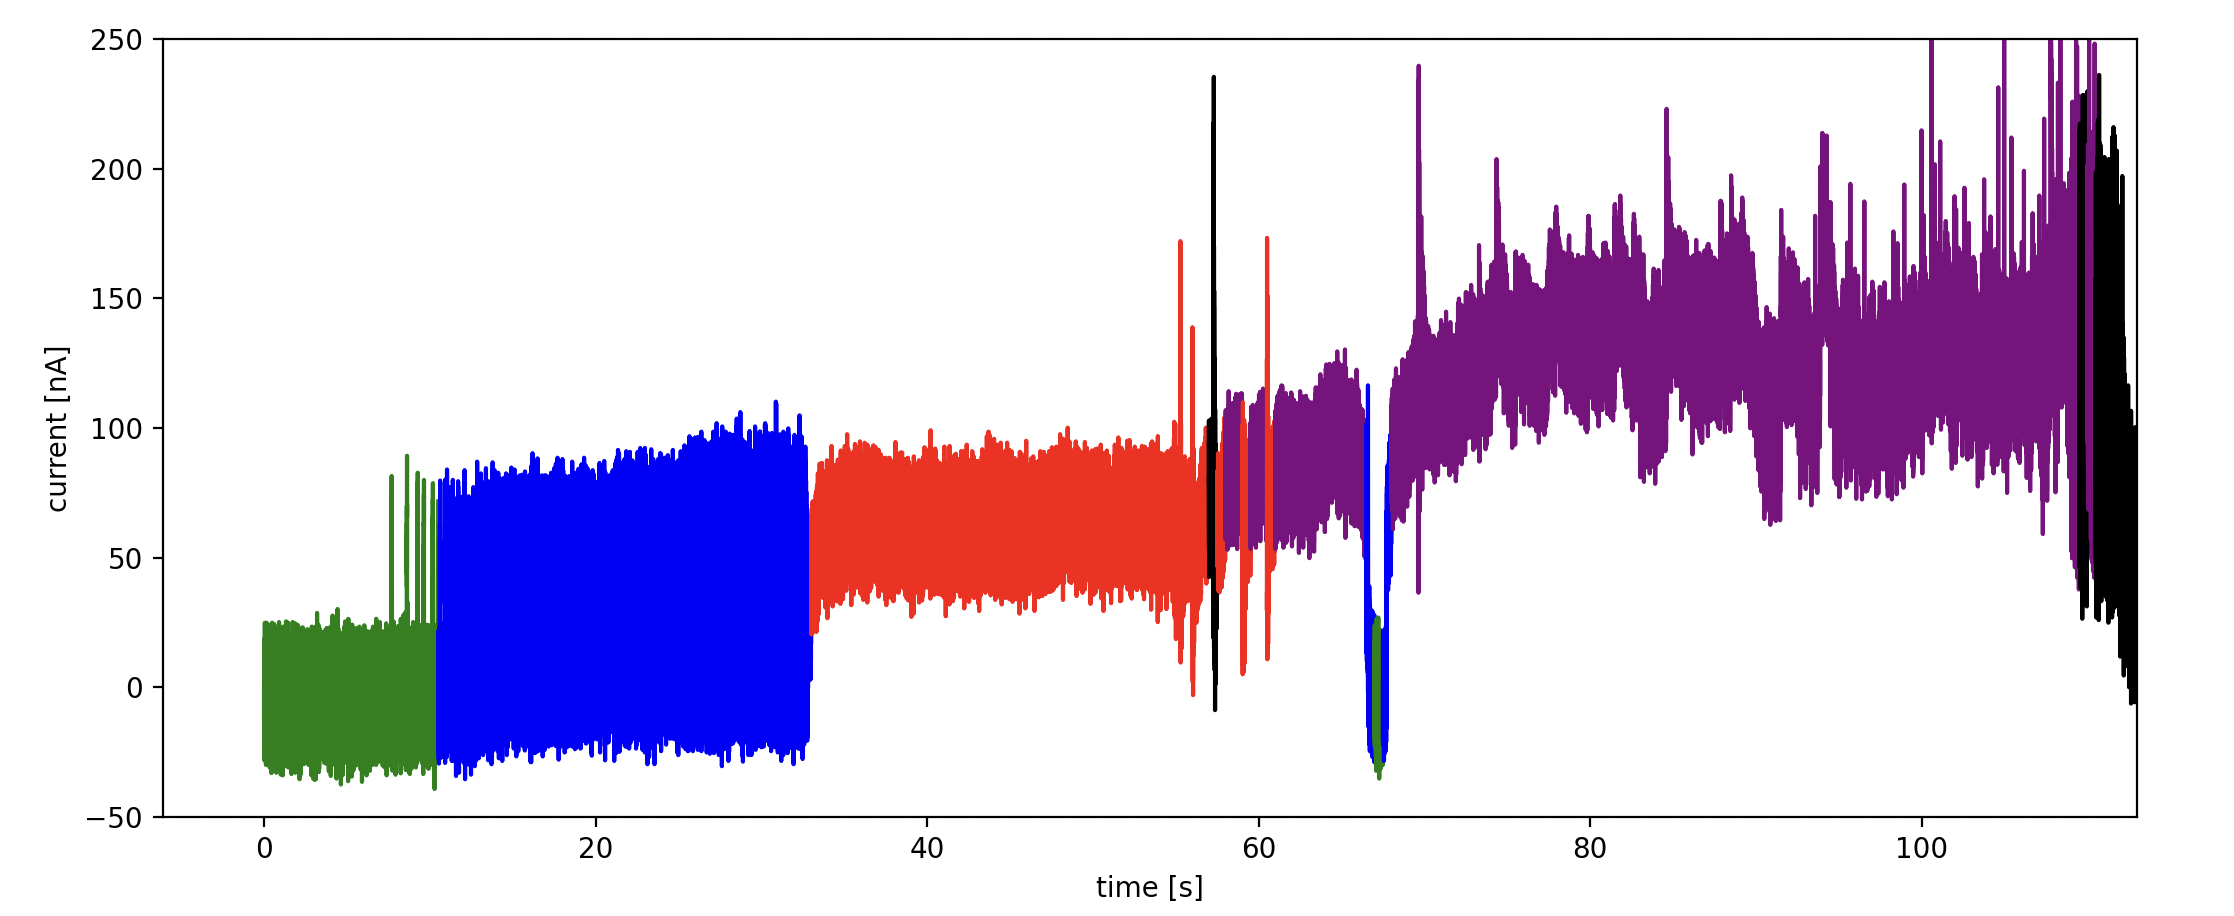
\includegraphics[width=12cm]{Figuras/19:03/classified-data-example.png}
    \caption{The same graph as \ref{fig:raw_data} but after the classification procedure. The colors are green: Dripping, Blue: Intermittent, Red: Cone Jet, Purple: Multi Jet and Black: Undefined.}
    \label{fig:class_step_data}
\end{figure}

The graph of voltage scan as showed in \ref{fig:raw_data} has a common shape for different liquids and parameters. After having familiarity with it is even possible to classify the spraying modes by visual analysis. For example: 
Dripping mode has a current mean of 0V. The Intermittent state has a high variation of values that can be seen by the thickness of the graph. The Cone jet is a thinner graph because the signal is more constant. The Multi Jet is the same as Cone jet graph but with a higher mean value than cone Jet. Corona sparks are not showed in the graph because the discharges has a high current value and will be above the axis limits.



\subsection{Map Sequence}
\label{subsec:map_results}

For validation purposes and also to expose the benefits of the automated routine and classification 




    For better understand the effects of both voltage and flow rate in the spraying dynamics manual experiments were made.
    Also in order to find the stability region of cone jet mode for the liquid and setup used.

    \begin{figure}[H]
        \center
        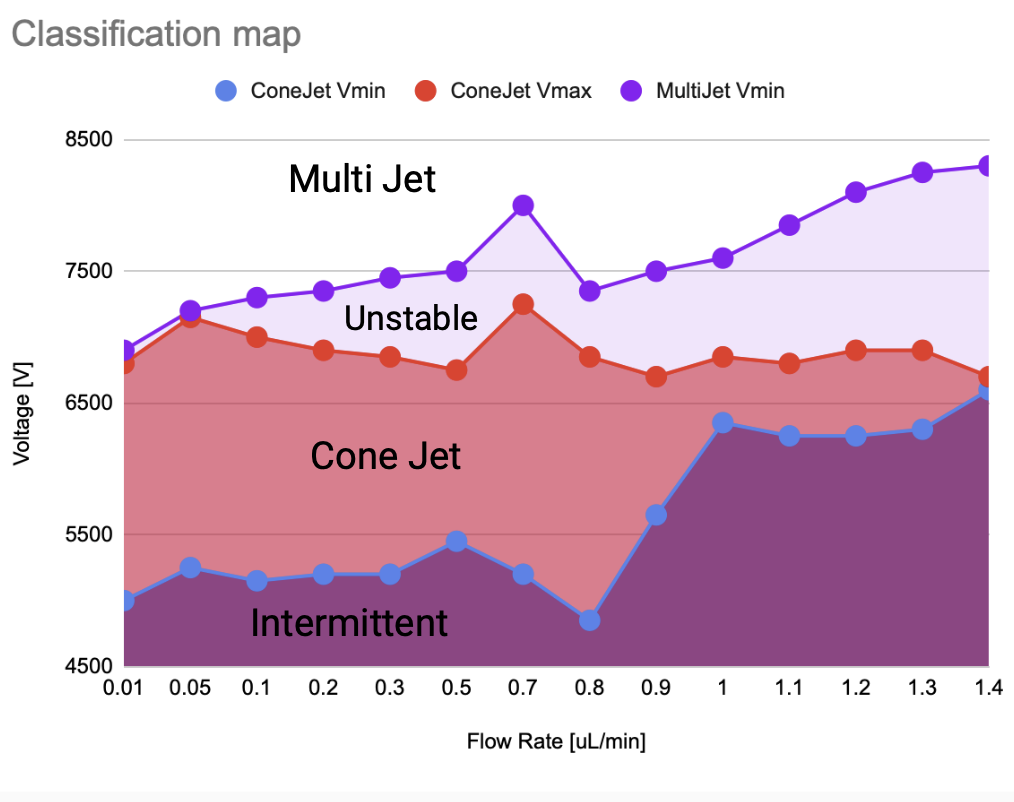
\includegraphics[width=12cm]{Figuras/regions.png}
        \caption{ exp-26-01-2 (V x Q)}
    \end{figure}


    For validation of the automatic system and classification some experiments were made having both manual and automatic data collecting.



    In Figure 14 we can see a result of the map generated by the automatic classification in this experiment.

    Figures 15 and 16 shows that we could achieve a stable cone jet region map with similar shape and values in both manual and automatic classification of the same experiment.

    \begin{multicols}{2}


        \begin{figure}[H]
            \center
            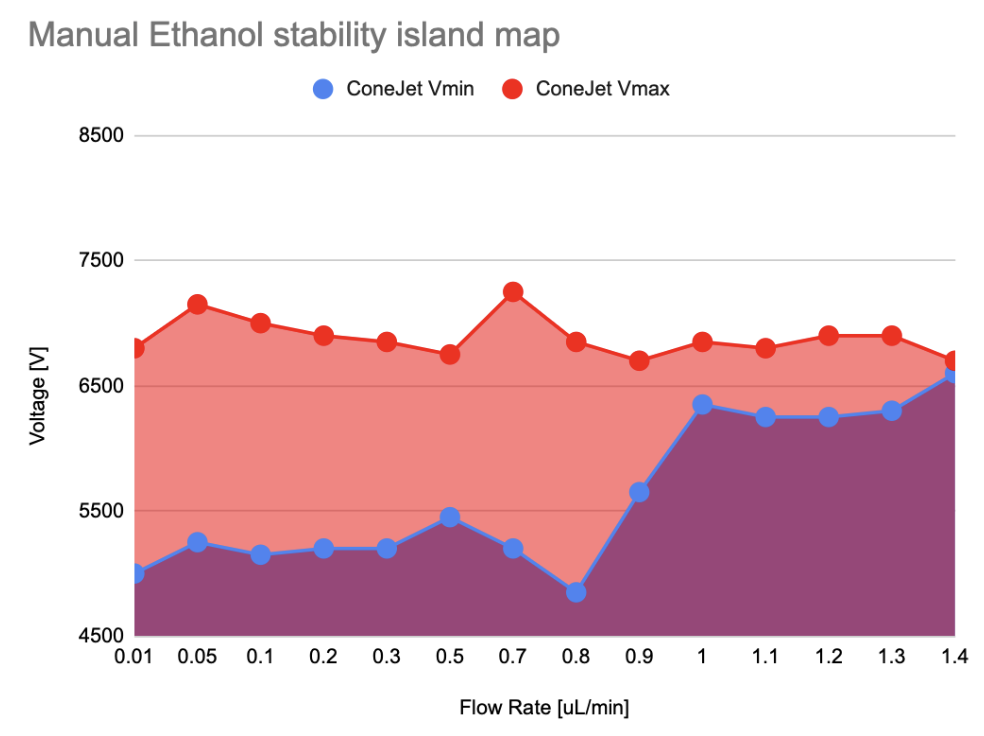
\includegraphics[width=8cm]{Figuras/april/manual_stability.png}
            \caption{ exp-26-01 manual classification}
        \end{figure}

        \begin{figure}[H]
            \center
            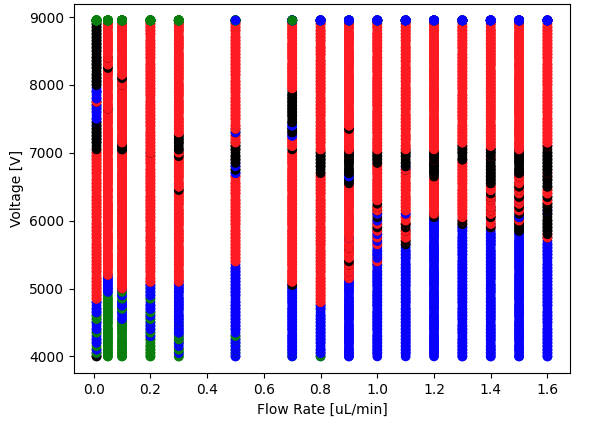
\includegraphics[width=9cm]{Figuras/report3/map-exp-26-01.png}
            \caption{ exp-26-01 automatic classification}
        \end{figure}

    \end{multicols}

    \begin{multicols}{2}


        \begin{figure}[H]
            \center
            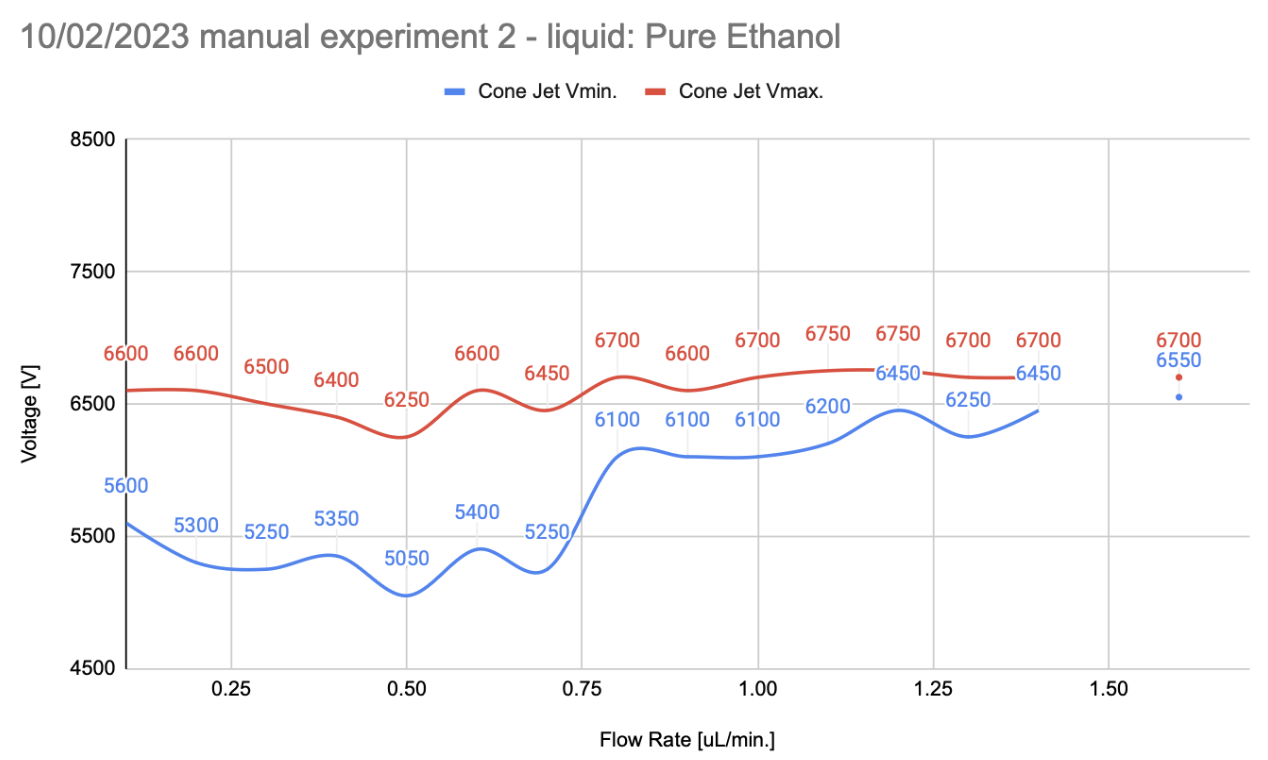
\includegraphics[width=8cm]{Figuras/april/results_map_1.png}
            \caption{ exp-26-01 manual classification}
        \end{figure}

        \begin{figure}[H]
            \center
            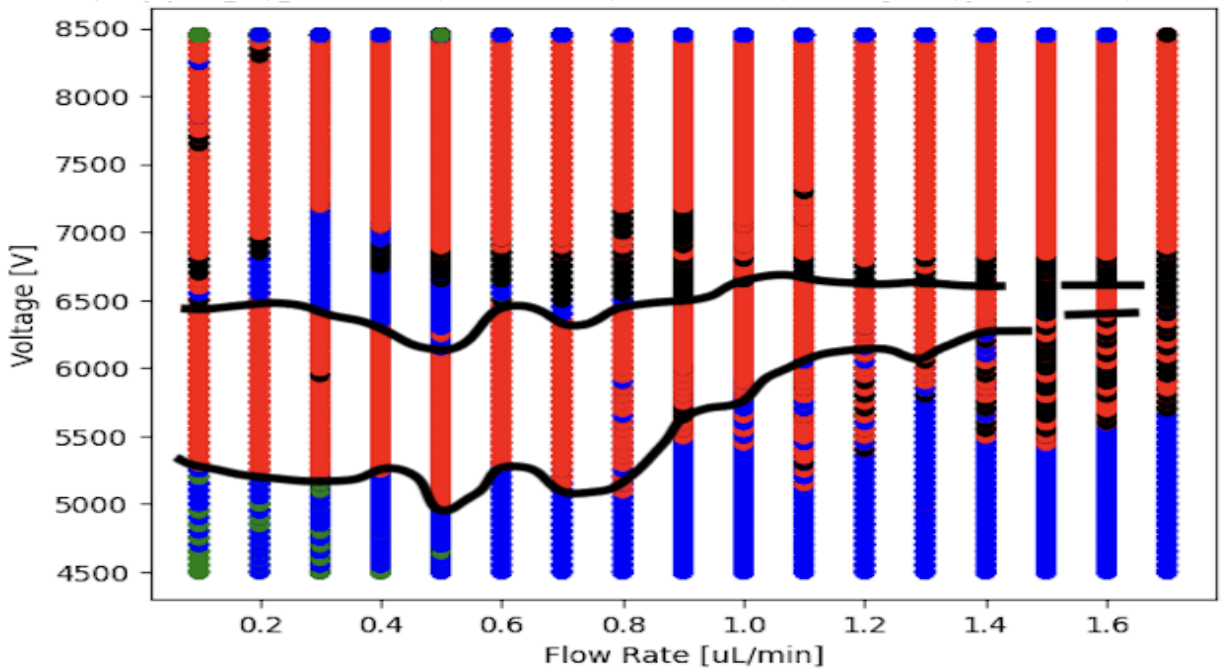
\includegraphics[width=9cm]{Figuras/april/results_map_2.png}
            \caption{ exp-26-01 automatic classification}
        \end{figure}

    \end{multicols}

    Figures 15 and 16 shows that we could achieve a stable cone jet region map with similar shape and values in both manual and automatic classification of the same experiment.


    \begin{multicols}{2}


        \begin{figure}[H]
            \center
            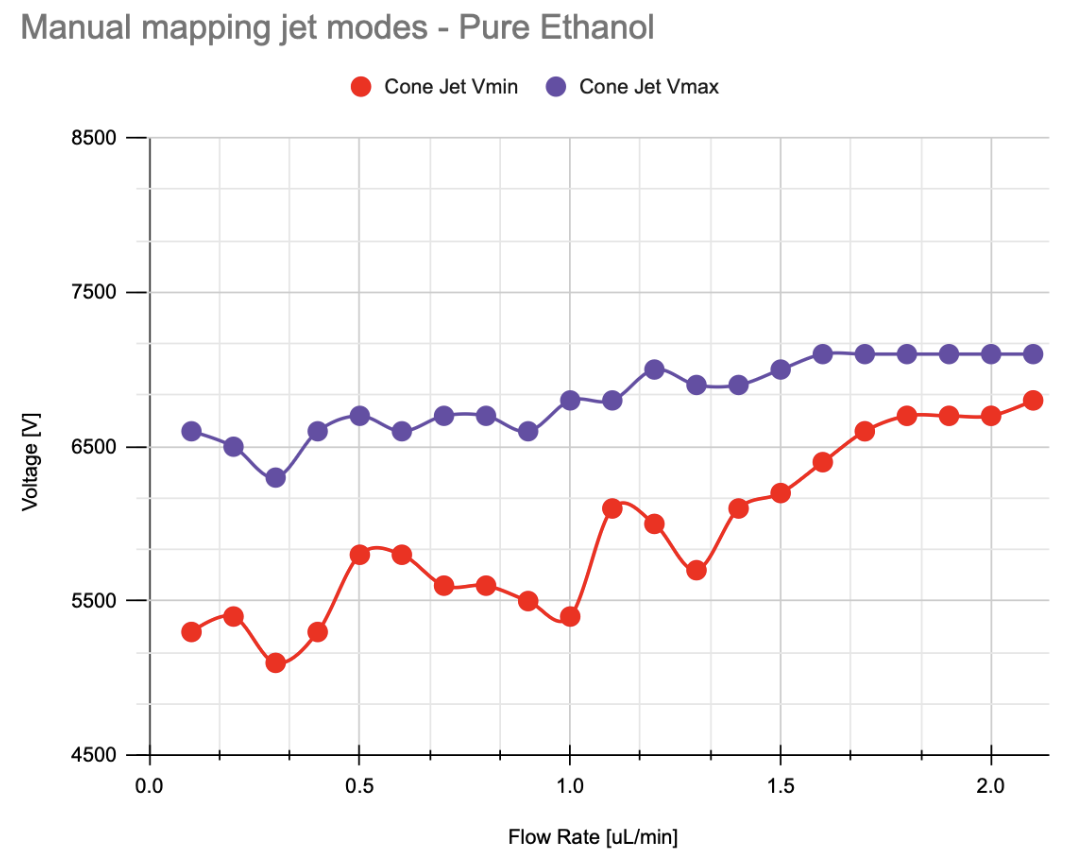
\includegraphics[width=8cm]{Figuras/april/map5.png}
            \caption{ exp-26-01 manual classification}
        \end{figure}

        \begin{figure}[H]
            \center
            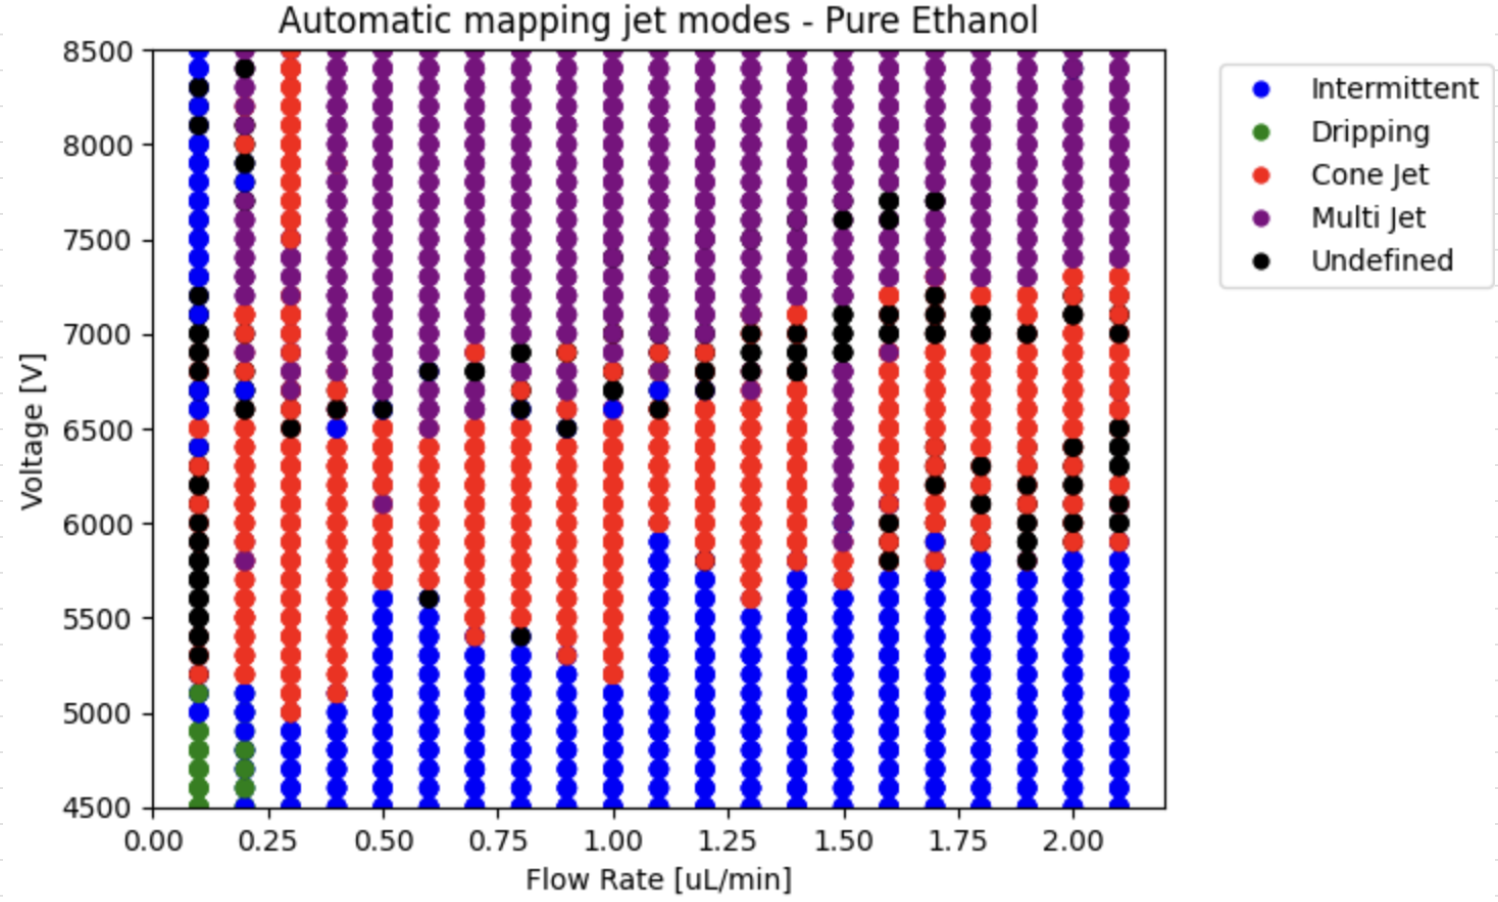
\includegraphics[width=10cm]{Figuras/april/map2.png}
            \caption{ exp-26-01 automatic classification}
        \end{figure}


    \end{multicols}

    \subsubsection{Non-dimensional axis}

    To compare with the literature and validate the algorithm we decided to display the data using the non-dimensional numbers used in figure \ref{fig:ganan_calvo_fig}.

    \begin{multicols}{2}

        \begin{figure}[H]
            \center
            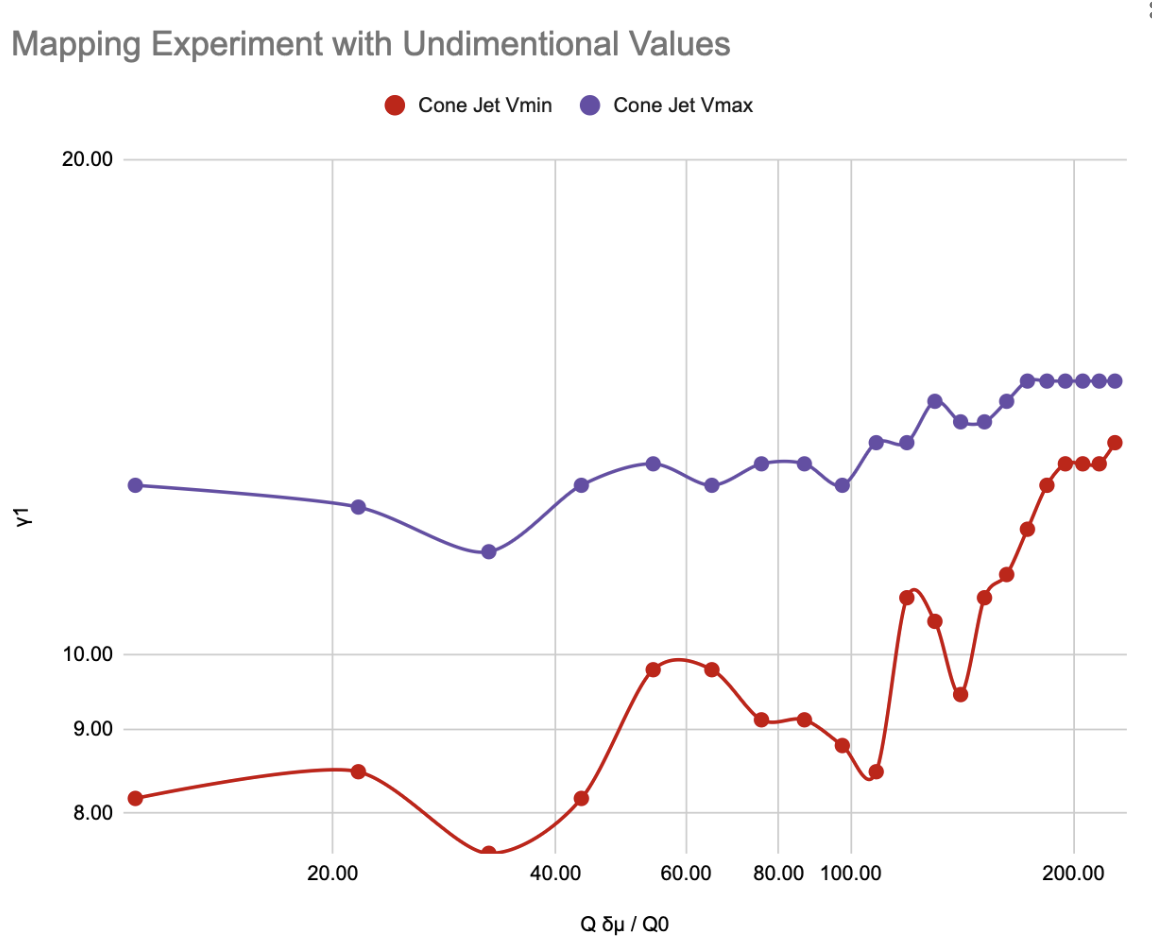
\includegraphics[width=7cm]{Figuras/april/manual_non_dim_exp.png}
            \caption{ exp-qw-01-2 (V x Q)}
        \end{figure}

        \begin{figure}[H]
            \center
            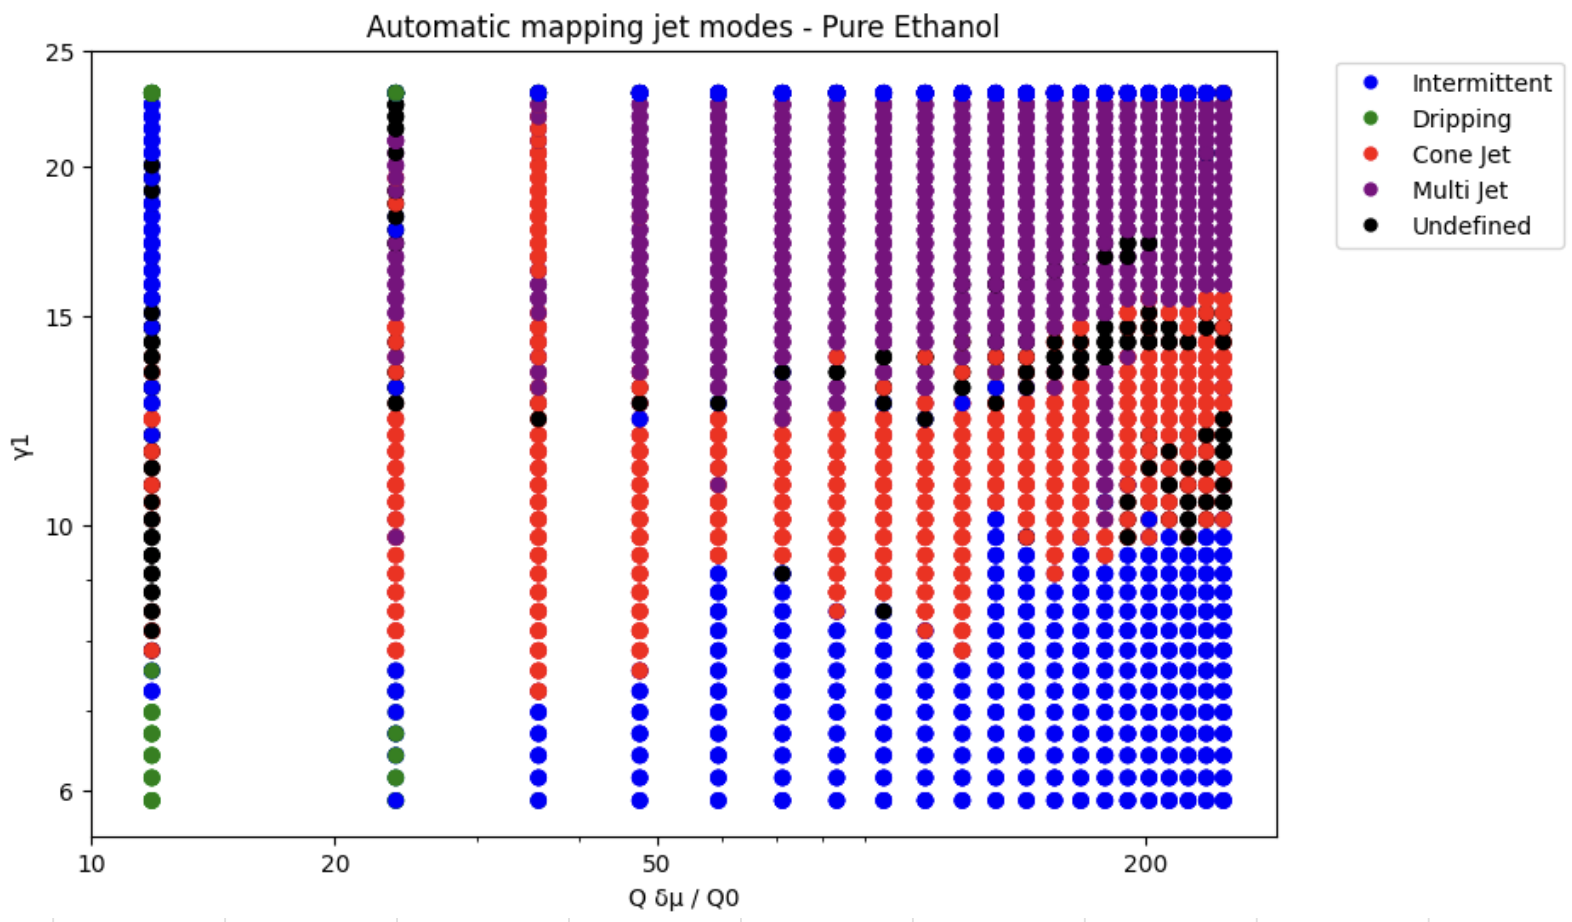
\includegraphics[width=10cm]{Figuras/19:03/non-dimensional-1.png}
            \caption{ exp-26-01-2 (V x Q)}
        \end{figure}


    \end{multicols}

\section{Controller}
\label{sec:controller_results}

    Of particular interest in applications is the cone-jet mode, where the meniscus emits a steady microscopic jet, resulting in uniformly sized droplets. 

        Flow rate perturbation robustness test

        \begin{figure}[H]
            \center
            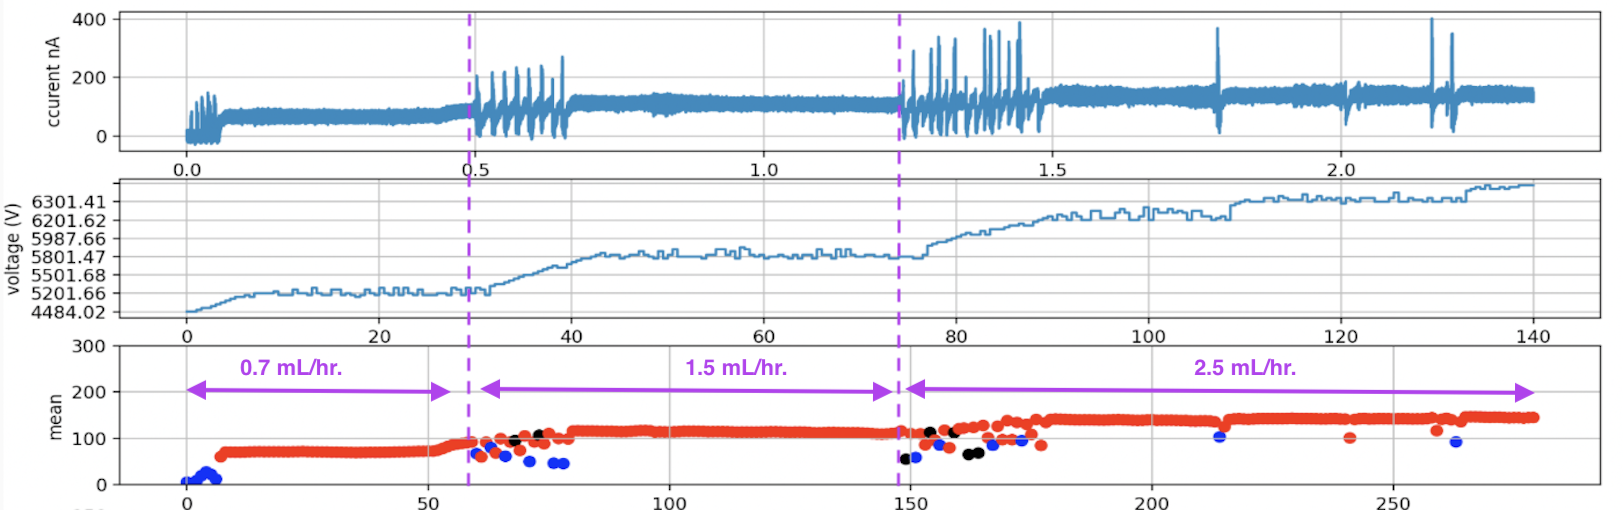
\includegraphics[width=17cm]{Figuras/19:03/control_first_results.png}
            \caption{ exp-26-01-2 (V x Q)}
        \end{figure}


    \subsection{Robust Controller}

    


    \section{System Portability}
    \label{sec:portability}
    
        Raspberry Pi


\clearpage
\chapter{Conclusion}
\label{chap:conclusion}

In conclusion, the implementation of a Python routine for complete automation and integration of the system has improved the precision of experiments and enabled real-time collection of extensive data without requiring the expertise and time of a specialized scientist. 
This project underscores the potential of automation in enhancing scientific research and accelerating progress towards achieving research goals.
In addition to its potential in scientific research, the software developed in this project can also be leveraged by industrial approaches. 
Furthermore, the classification methods and system control implemented in this project have yielded promising results and can be further optimized in the future. Overall, this project serves as a contribution towards the advancement of automated systems and the optimization of experimental processes.

\section{Proposal for continuation}

To continue, my proposal would be to prioritize the improvement of the classification step. 
Ideally, we could use machine learning or another algorithm to ensure accurate classification with a broad range of liquids.
By achieving a reliable classification, we can then implement more effective controller logic or approaches. 
In this regard, I would like to present the concept of a fuzzy controller as a potential solution.

\subsection{Machine Learning}

    When it comes to classifying spraying modes, machine learning represents a sophisticated and trendy approach.
    This project was designed in order to substitute our statistical classifier for a more general and accurate algorithm.
    
    The data collected in this project was saved in 0.5s samples together with its classification allowing it to be used for supervised learning.
    Experimental trials were conducted to explore machine learning algorithms to classify the data. Unfortunately, despite efforts, an accurate method of distinguishing between classifications could not be identified.

\subsection{Fuzzy Controller}

        One challenge in implementing the controller in this project is that we don't have a real value as feedback, instead, the feedback from the controller loop is a classification, which makes it difficult to apply many of the principles of control theory that are designed for continuous control. 
        As this project involves logical control, it requires a different approach. 
        
        The controller project that will be presented is an attempt to quantify the classification and fit it in a fuzzy control model.
        That approach is for an open loop control system and the input and outputs of the controller must be fuzzyfied.

        Firstly, the fuzzyfication and defuzzyfication machines were implemented using the data acquired in the experiment of step routine\ref{subsec:step_routine}, mapping the area of each spraying mode according to its potential.
        Figure \ref{fig:fuzzyy} shows the steps of fuzzyfication and defuzzyfication within the input and output of the controller.


            \begin{figure}[H]
                \centering
                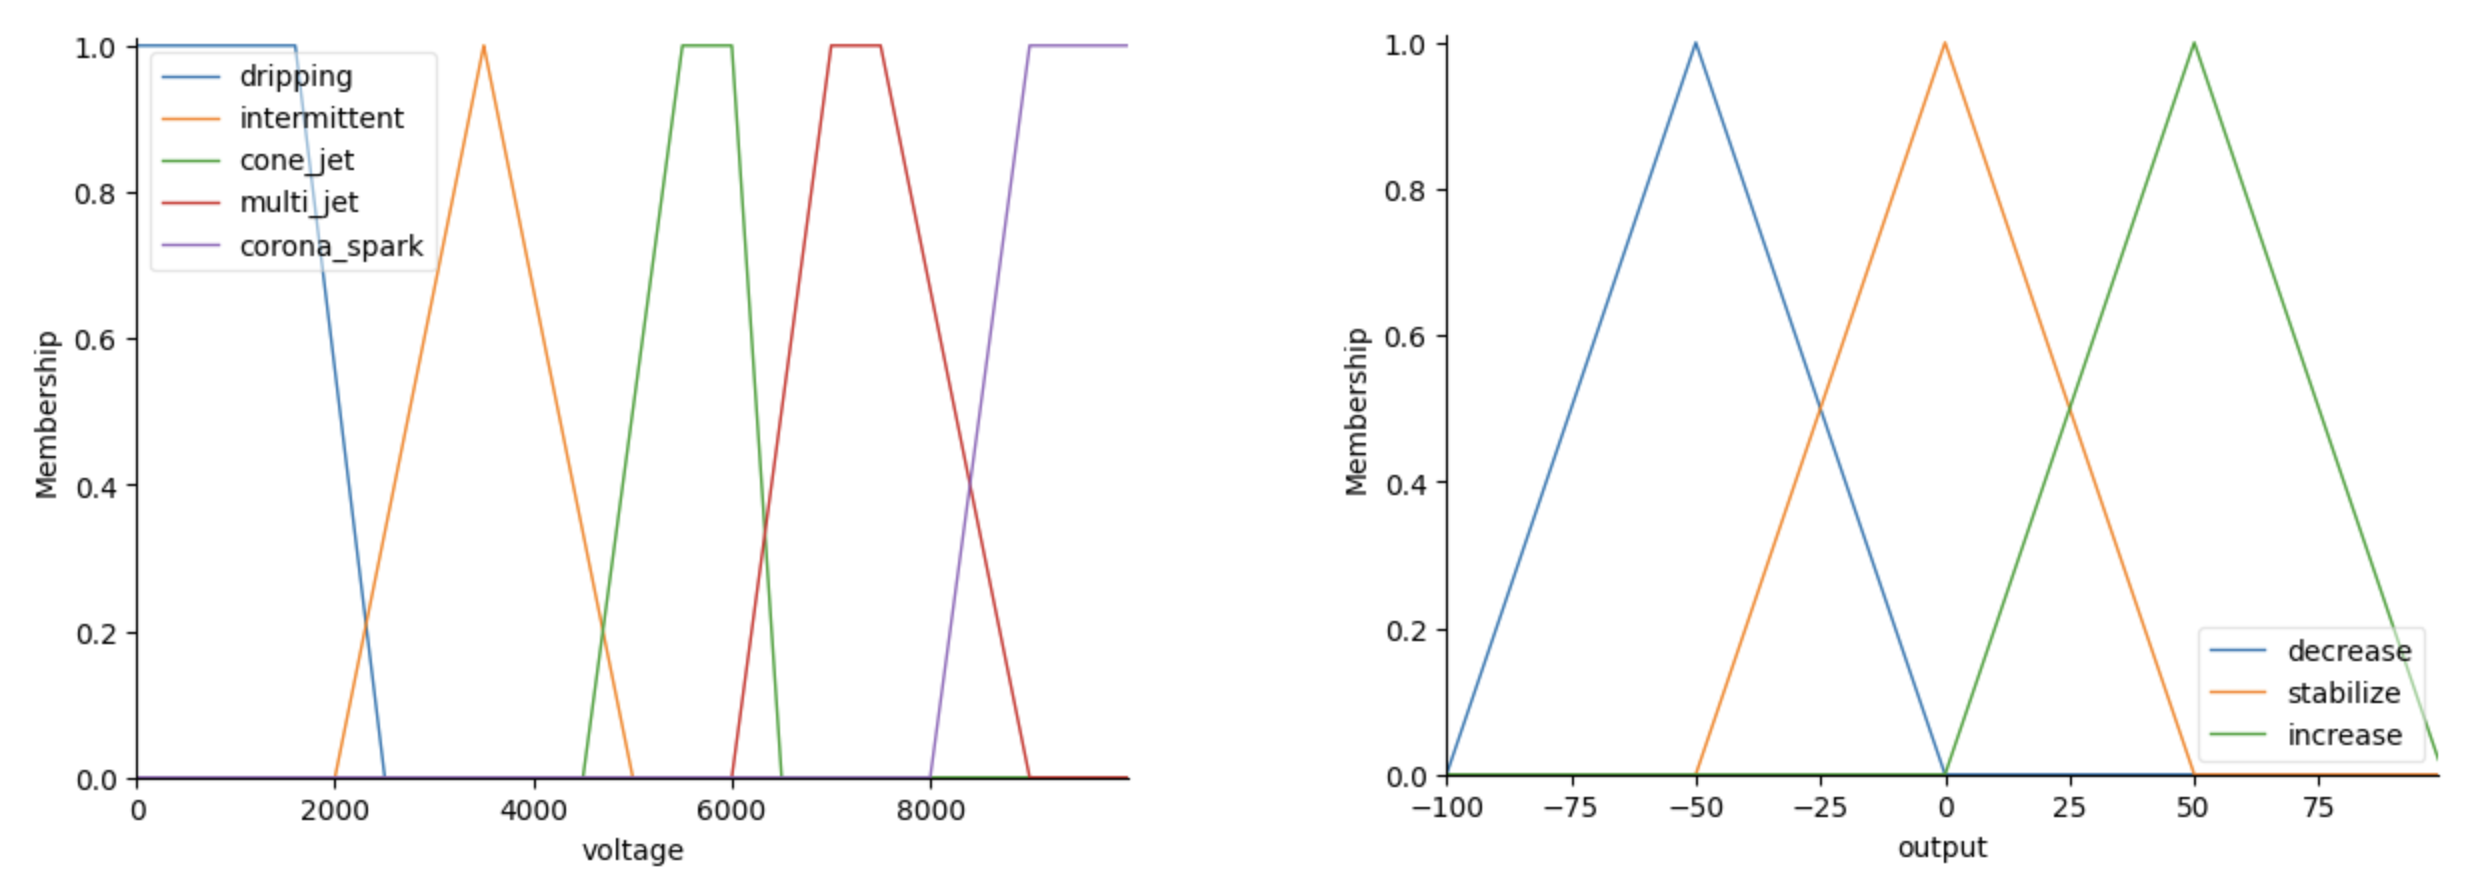
\includegraphics[width=17cm]{Figuras/fuzzy/Fuzzyy.png}
                \caption{fuzzyfication of input and defuzzyfication of output}
                \label{fig:fuzzyy}
            \end{figure}



        Our controller is an algorithm that calculate the output with a geometrical calculus on the membership functions of the input and output according to our rules listed below.

        Fuzzy Rules:

        -> IF dripping THEN increase

        -> IF intermittent THEN increase

        -> IF cone jet THEN stabilize

        -> IF multi jet THEN decrease

        -> IF corona THEN decrease


        In figure \ref{fig:fuzzyy1}, two tests were made. Test 1 with a higher voltage of 7000V accusing it to be 100\% in multi jet and the output of decrease voltage. Test 2 shows the opposite case when the voltage is lower than expected.

    \begin{figure}[H]
        \centering
        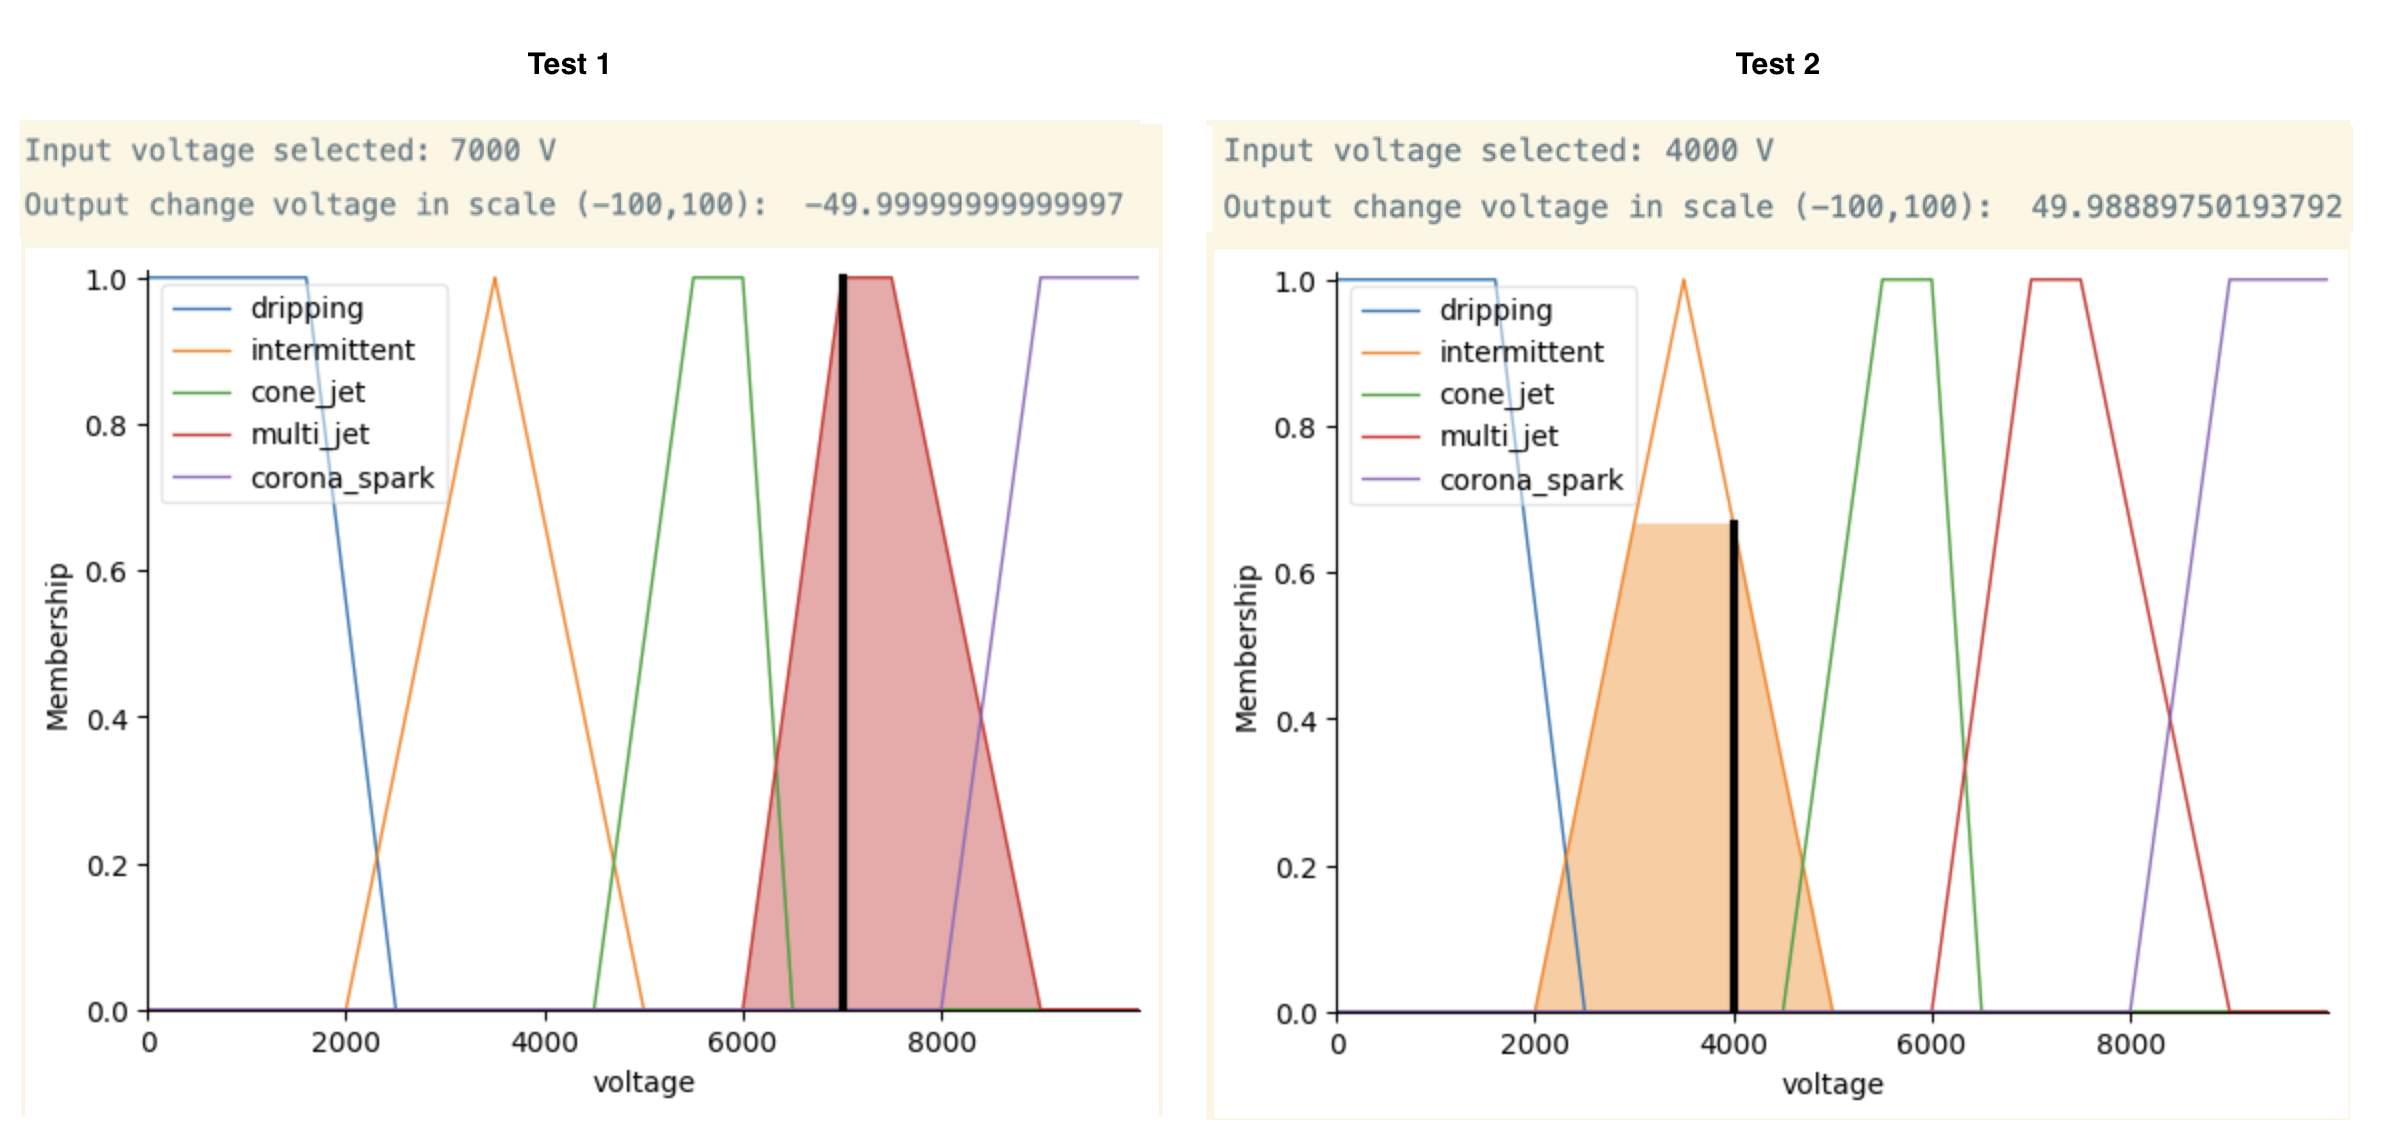
\includegraphics[width=17cm]{Figuras/fuzzy/test3.png}
        \caption{Test implemented to validate the concept of fuzzy controller in this project.}
        \label{fig:fuzzyy1}
    \end{figure}
        

    \section{Final Discussions}

        The works presented in this report represent a continuation and refinement of previous efforts to develop a more precise and versatile automation routine that can be effectively applied in both industrial and research applications. 
        
        The previous student work focused on predicting corona streamers or spark discharges\cite{Monica} and her automation routine provided a valuable proof-of-concept. 
        
        The current project builds on this foundation and highlights several key results, including the integration of a liquid pump into the software and the development of a routine that can be easily modeled to fit a control model, making it straightforward to implement new control algorithms or experiment routines. 
        The software was also remodeled to support threads, allowing for the separation of each subsystem and the exchange of data between them using queue data structures. A classification for multi-jet spraying mode was developed, along with a simple controller to demonstrate proof of concept. 
        Additionally, the saving of data was optimized to a real-time streaming format and expanded to include more sensor data. Finally, the algorithm usability was restructured to make it more intuitive for users through the use of a setup file.

        
\clearpage


\addcontentsline{toc}{chapter}{Bibliography}
\renewcommand{\bibname}{References}

%\bibliographystyle{abntex2-alf} %para norma ABNT no sistema autor-data
\bibliographystyle{abntex2-num}
\begin{small}
\bibliography{ListadeReferencias}%,library}
%% Monografia para Projeto de Fim de Curso - Exemplo no LaTeX
%-----------------------------------------------------------


%---------------Inicialização de pacotes--------------------

\documentclass[12pt,a4paper,notitlepage,twoside]{book}


\usepackage{graphicx}
\usepackage[utf8]{inputenc}
%\usepackage[latin1]{inputenc} %%pode ser necessário trocar a codificação em sistemas Windows
\usepackage[brazil]{babel}		%%pode ser necessário trocar o pacote de línguas em algumas distribuições LateX
%\usepackage[portuguese]{babel}
\usepackage[T1]{fontenc}
\usepackage{amsmath,amssymb}
\usepackage{amsthm,amsfonts}
\usepackage{color}
\usepackage[colorlinks]{hyperref}
\usepackage{abntex2abrev}
%\usepackage[alf]{abntex2cite} %se você quiser seguir as normas ABNT no sistema autor-data
%\usepackage[num]{abntex2cite} %se você quiser seguir as normas ABNT no sistema numérico
\usepackage{setspace}
\usepackage[toc,page]{appendix}

%Definindo fonte Times (Use os pacotes obsoletos se não conseguir instalar os atualizados)
%\usepackage{times}     %Pacote de fontes obsoleto, apenas texto
%usepackage{mathptmx}  %Pacote de fontes obsoleto, texto e símbolos matemáticos
%\usepackage{newtxtext,newtxmath}  %Pacotes de fontes mais recentes

\usepackage[a4paper,top=30mm,bottom=30mm,inner=30mm,outer=25mm,headheight=7mm,headsep=6mm,footskip=7mm]{geometry}
\usepackage{enumerate}

\makeindex

%\singlespacing   %%espaçamento simples
%\onehalfspacing
%\setstretch{1.03} %%um pouco melhor que espaçamento simples
\linespread{1.25} %corresponde ao espaçamento 1.5 do MS Word

%---------------Início do documento-------------------------

\begin{document}

\begin{titlepage}
    \begin{center}
           
    \begin{figure}
            \centering
            % \subfigure{
\includegraphics[width=5cm]{Figuras/wac.png}}
            \hspace{0.1\textwidth}
            \subfigure{
\includegraphics[width=6cm]{Figuras/nhl-stenden.png}}
            \vspace{3cm} 
        \end{figure}

    

    {\bf\Large EHDA closed loop control system based on real time non-visual spray mode classification\\}
    \vspace{1cm} 
    {\Large Report}
    \vspace{2cm}  
    
    %\hspace{0.3\textwidth} 
    {\bf\large Student: João Pedro Miranda Marques}\\
    \vspace{2cm}
    {\large Supervisors:\\ Luewton L F Agostinho\\
            Klaus Glanzer \\
            Antônio Carrasco}
    \vspace{2cm}  

    \today
    \vspace{2cm}  
       

    %\hspace{0.3\textwidth} 
    \large \date{\today}
    \end{center}
    
    \end{titlepage}



\title{
    EHDA closed loop control system based on real time non-visual spray mode classification \\
    \large Relatório de Atividades}


\pagenumbering{roman}
\addcontentsline{toc}{chapter}{Resumo}

\begin{center}
\huge{{\bf Resumo}}
\vspace{2cm}
\end{center}

A Atomização Eletro-hidrodinâmica (EHDA), também chamada de electrospray, é uma técnica de atomização de líquidos que produz gotículas de dimensão micro e nanométricas, utilizando campos elétricos elevados (kV/cm).
De acordo com Cloupeau e Prunet-Foch\cite{prunet} (1994) , os electrosprays podem gerar gotículas em diferentes dinâmicas, que os autores denominaram "modos de electrospray". 
 Esses modos podem ser ajustados variando a força do campo elétrico e a vazão de líquido, mas também dependem da geometria e das propriedades físico químicas sistema. 
 Em seu trabalho, os autores propuseram quatro possíveis modos EHDA: gotejamento, intermitente, jato cone e jato multi, que são geralmente distinguíveis visualmente.
 Verdoold et al.\cite{Sjaaks} (2014) sugeriram recentemente uma abordagem de classificação com base no comportamento da corrente elétrica do processo de electrospray.

Este projeto desenvolve um método de controle em malha fechada para dispositivos EHDA que utiliza classificação de modo de spray em tempo real com base em corrente elétrica (portanto, não visual). 
O projeto de sistema de electrospray é totalmente automático, onde todos os periféricos, como fonte de alimentação HV e bomba de seringa, são controlados por um computador que executa suas rotinas. 
O sistema classifica a dinâmica do modo de spray usando dados de corrente em tempo real e altera os parâmetros operacionais do EHDA, como vazão do líquido e tensão aplicada, para alcançar e manter o modo de spray escolhido. 
Os modos de electrospray são validados em tempo real usando uma câmera de alta velocidade.
Em comparação com as abordagens manuais convencionais, o algoritmo de controle implementado alcança maior precisão e menor tempo de transição. 
Portanto, um sistema EHDA completamente autônomo abre portas para potenciais aplicações industriais. 
Além disso, o uso do sinal de corrente elétrica será útil para estudar mais a fundo os processos de electrospray, levando a um melhor controle na geração de gotículas (frequência, tamanho e carga). 
A incorporação de Aprendizado de Máquina para melhorar a categorização de modos será um desenvolvimento futuro.

\clearpage
\thispagestyle{empty}
\cleardoublepage

% No Resumo, em uma única página, em no máximo dois parágrafos, você explicita os seguintes itens: objetivos do projeto e descrição sucinta do local onde ele foi desenvolvido; metodologia utilizada; e resultados alcançados. Leitores experientes decidem se prosseguirão para a leitura do texto completo após lerem o resumo, a conclusão e a introdução. Por isso nestes lugares você deve colocar um esforço maior de convencimento. Além disso, a linguagem utilizada deve ser acessível a leitores com pouca familiaridade com a área, limitando-se o uso de jargões.
 
% \begin{sloppypar}
% Este novo parágrafo serve para mostrar que ao pular uma ou mais linhas no texto do arquivo .tex, o \TeX\ entende que você está iniciando outro parágrafo. O comando \textsf{sloppypar} força o texto a não ultrapassar as margens. Só deve ser usado se este problema ocorrer.
% \end{sloppypar}

\addcontentsline{toc}{chapter}{Abstract}

\begin{center}
\huge{{\bf Abstract}}
\vspace{2cm}
\end{center}

    Electrohydrodynamic Atomization (EHDA), also called electrospray, is a liquid atomization technique that
    produces micro and nanometric charged droplets within a narrow size distribution by using high electric fields (kV/cm).
    According to Cloupeau and Prunet-Foch\cite{prunet} (1994), electrosprays can generate droplets in different ways, which the authors
    named "electrospray modes". These modes may be adjusted by varying the strength of the electric field and flow rate,
    but also depend on liquid properties and system geometry. In their work, the authors proposed four possible EHDA
    modes: dripping, intermittent, cone-jet and multi-jet, which are generally distinguished visually.
    
    This project develops a closed-loop control method for EHDA devices that uses real-time, electric current-based (hence
    non-visual) spray mode classification.
    The proposed electrospray system is entirely automatic, where all the peripherals, such as HV power supply and syringe
    pump, are controlled by a computer which executes their routines.
    The system classifies spray mode dynamics using real-time current data and changes EHDA operating parameters such
    as liquid flow rate and applied voltage to achieve and maintain the chosen spray mode. The electrospray modes are
    validated in real time by using a high-speed camera.
    As compared to conventional manual approaches, the control algorithm promises higher
    accuracy and lower transient time. Therefore, a completely autonomous EHDA system opens the door to potential
    industrial applications. In addition, the use of the electric current signal can be useful to further research in electrospray
    processes, leading to better control on droplet generation (frequency, size and charge).
 

\addcontentsline{toc}{chapter}{Agradecimentos}

\begin{center}
\huge{{\bf Agradecimentos}}
\vspace{4cm}
\end{center}

Um Agradecimento a minha mãe que sempre me apoiou e me fez acreditar no meu potencial. Me ensinando dedicacao, paciencia e disciplina.
Ao meu pai me que ensinou a não estar satisfeito e buscar sempre mais, isso que eu chamo de ambicão e energia para sempre buscar sair da zona de conforto.
Aos meus queridos amigos da República Casassanta por terem tornado a vida universitária esse momento tão único e inesquecível.
 
\clearpage
\thispagestyle{empty}
\cleardoublepage
\tableofcontents
%\markboth{Conteúdo}{Conteúdo}

\clearpage
%\thispagestyle{empty}
%\cleardoublepage

% Normalmente, este arquivo só contém isto.
\listoffigures
\addcontentsline{toc}{chapter}{List of Figures}
%\markboth{Lista de Figuras}{Lista de Figuras}

\clearpage
%\thispagestyle{empty}
%\cleardoublepage

% Normalmente, este arquivo só contém isto.
% \listoftables
\listofalgorithms
\addcontentsline{toc}{chapter}{Lista de Tabelas}
%\markboth{Lista de Tabelas}{Lista de Tabelas}

\clearpage
%\thispagestyle{empty}
%\cleardoublepage

% Normalmente, este arquivo só contém isto.

\pagenumbering{arabic}
\setcounter{page}{1}
\chapter{Introduction}
\label{chap:intro} %este label será usado para referenciar este capítulo

A atomização eletrohidrodinâmica (EHDA), também conhecida como eletrospray (ES), é uma maneira de desintegrar um líquido
em gotículas, expondo-o a um forte campo elétrico. 


% As primeiras frases têm a missão de prender a atenção do leitor e por isso são as mais importantes do texto. Diga o quanto antes o que você fez e quais são os resultados alcançados. Ao terminar de ler a introdução o leitor tomará uma nova decisão de se vale a pena ou não continuar lendo o texto. Capte a atenção do leitor bem aqui.

% A comunicação escrita é considerada umas das cinco habilidades mais importantes por profissionais de engenharia e um engenheiro passa em média mais de $25$\% do seu tempo escrevendo \cite{eggert2002response,spretnak1982survey}. Uma quantidade similar de tempo é gasta na escrita de correspondência e de relatórios técnicos \cite{cunningham2012perceptions}. Dessa forma, encare a escrita do seu projeto como um treinamento nessa importante habilidade.

% Neste texto você encontrará não apenas uma estrutura para escrever seu trabalho em \LaTeX, mas também um pequeno manual de boas práticas na escrita técnica. Leia com atenção e coloque as sugestões em prática à medida que preenche o texto com o conteúdo do seu próprio projeto. Também será apresentado um número de vícios de escrita comumente encontrados nas monografias de alunos. 

% A seguir está a estrutura de organização sugerida pelo colegiado do curso. Note que ela não é necessariamente a melhor para contar a história do seu projeto. Você pode por exemplo preferir usar títulos mais pertinentes ao seu contexto. Contudo, o seu texto deve conter cada um dos pontos a seguir.

\section{Motivation and Justify}
\label{sec:motivacao}
% Argumente sobre a importância do projeto desenvolvido usando uma visão de alto nível, sem entrar em detalhes. Contextualize seu projeto dentro do local de execução ou da literatura e explique como ele é necessário ou inovador. É possível fazer uma breve revisão bibliográfica, confrontando seu trabalho com outras referências bibliográficas para mostrar a sua contribuição. No quesito contribuição, é muito importante deixar claro o tempo todo que partes do projetos foram executadas por outros e que partes foram executadas por você. Caso contrário, corre-se o risco de inadvertidademente tomar crédito pelo trabalho de outrem, o que pode ter implicações legais. 

As pesquisas de EHDA têm contribuído como uma importante ferramenta para
o desenvolvimento da tecnologia da água (dessalinização térmica e recuperação de metais), ciências dos materiais (nanofibras e
fabricação de nanoesferas, recuperação de metal, membranas seletivas e baterias) e aplicação biomédica
(encapsulamento). Além disso, o projeto está integrado à estratégia de Transição Energética e à Agenda de Inovação
Agricultura, água e alimentos, tecnologias facilitadoras essenciais (KETs). Embora existam aplicações de EHDA em
indústria, a estabilização do modo de pulverização de jato cônico é feita empiricamente e com base em medições de corrente média.
A corrente elétrica que flui transportada pelo spray revela formas características para diferentes modos de atomização.
Essas formas não podem ser simplesmente resumidas por seu valor médio. Na figura um podemos ver um exemplo de cone-jet
modo eletrospray.

Figura 1: exemplo de EHDA

As técnicas de processamento de sinal podem permitir uma classificação não visual do modo de pulverização com base no elétrico
forma atual. O processo de pulverização impõe ruídos e sequências aleatórias no sinal medido tornando-o
classificação não é uma tarefa trivial.
Aplicações industriais exigem estabilização automatizada de um modo de pulverização. Isso pode ser obtido por um sistema fechado
sistema de controle de circuito. A classificação automatizada do modo de pulverização é uma parte crucial de um sistema de controle, assim como
o desenvolvimento de um algoritmo de controle apropriado.

\section{Project objectives}
\label{sec:objetivos}

Tendo em vista o exposto acima, este projeto tem por objetivos:

\begin{enumerate}[a)]
\item Item 1;
\item Item 2; 
\item Etc.     
\end{enumerate}

O conteúdo desta seção pode se sobrepor um pouco com o da seção anterior, podendo ela ser um sumário dos pontos expostos anteriormente. A escolha do título da seção talvez seja mais apropriada para a fase de proposta do projeto. Afinal, nesta fase se conhecem os objetivos e não os resultados. Por outro lado, fará pouco sentido discutir objetivos quando o projeto está finalizado, especialmente se tais objetivos não foram alcançados. 


\section{People envolved}
\label{sec:empresa}

% Faça uma breve apresentação da empresa ou laboratório onde o projeto é desenvolvido. Fale um pouco da história da empresa, do mercado em que atua, da sua organização, do departamento em que está inserido o projeto, etc. Descreva também o seu vínculo com a empresa. 
Implementações de processamento de sinal de projetos anteriores
do grupo NHL Stenden Water Technology estão mostrando bons resultados de classificação. Mais pesquisas são
necessário para melhorar a precisão da classificação e pesquisa e implementação de uma classificação adequada
algoritmo. Por causa disso, o trabalho será feito pelo Water Technology Group da NHL Stenden University
de Ciências Aplicadas e em combinação com empresas holandesas para combinar possibilidades de análise com conhecimento
e disponibilidade de infraestrutura.


\clearpage
\chapter[Descrição do Processo]{Descrição do Problema/Processo ou O Processo de Fazer Alguma Coisa}
\label{chap:descricaoproblema}
%Note que, como nome do capítulo é muito longo, fornecemos um nome abreviado uso no cabeçalho

Se desejar, uma visão geral do capítulo pode ser colocada antes da primeira seção. Este é o capítulo de descrição do processo e formulação do problema. Tendo em vista que se trata de uma monografia de engenharia de controle e automação, em muitos casos será fundamental a apresentação dos sensores e atuadores do processo.


\section{Processo de Fazer Alguma Coisa}
\label{sec:hist}

Cada seção inicia pela descrição do seu conteúdo e pode terminar com um parágrafo de conexão com a seção seguinte. 

Antes de formular o problema, \textbf{não se esqueça de fazer todas as definições necessárias}. Também devem-se detalhar os aspectos complementares da abordagem: se estamos estudando um aspeto particular do problema, se a resposta encontrada é universal ou dependente de simplificações e hipóteses prévias.


\section{Instrumentação do Processo}
\label{sec:instrumentação}

Descreva a aparelhagem e o equipamento utilizados bem como a ligação entre os diversos componentes. Nesta seção e, ao longo de todo o texto, você deve dar detalhes suficientes para que qualquer pessoa consiga reproduzir seus experimentos.

Contudo, \textbf{não disperse o leitor com detalhes irrelevantes} ou aspectos
demasiado técnicos ou formais. Reserve tais detalhes para um
apêndice.

Como uma imagem vale mais que mil palavras, e como usar mil palavras prejudicaria a clareza do texto, ilustramos o processo com a Figura \ref{fig:processo}. Lembrar que toda figura deve ser comentada no texto, você nunca deve colocar figuras que fiquem ``soltas'' no texto.  

\begin{figure}[thpb]
  \centering
  \resizebox{120mm}{!}{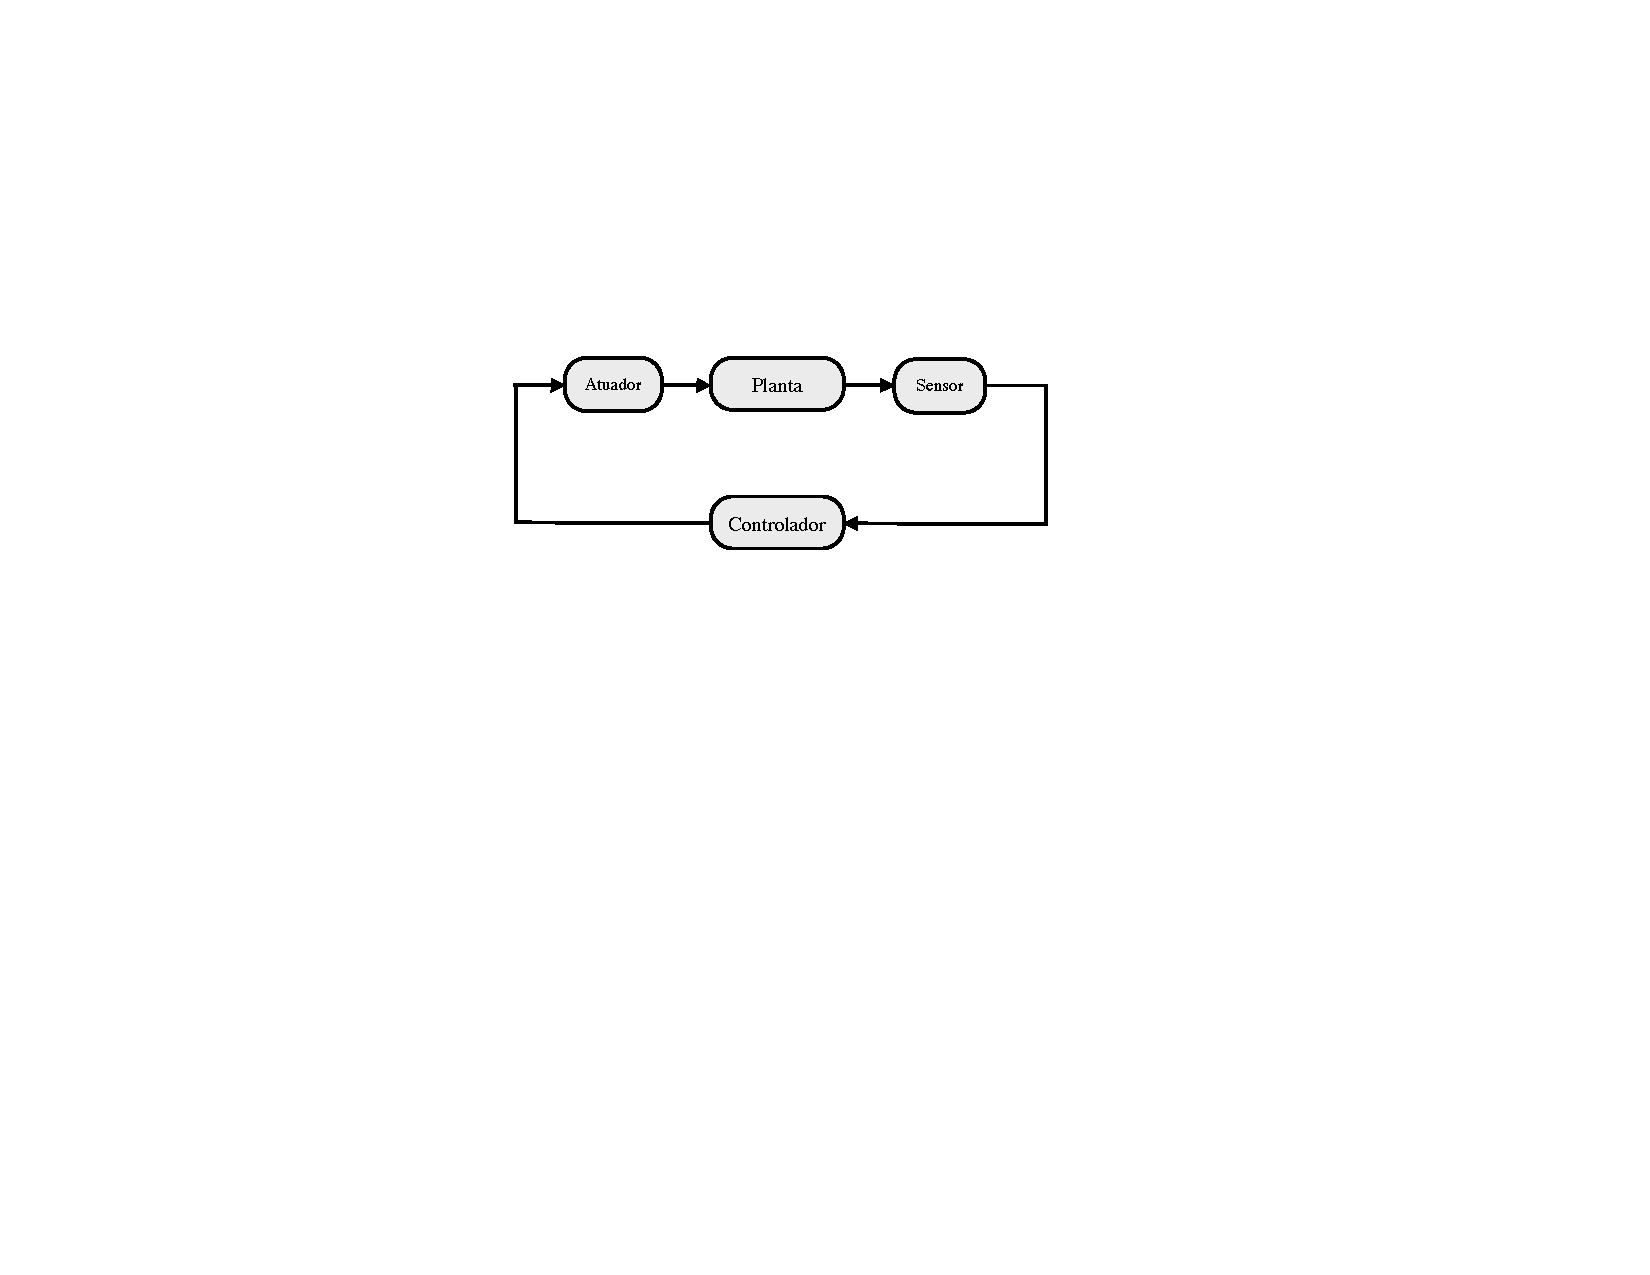
\includegraphics{DescricaoProcesso/Figuras/FiguraProcesso.pdf}}
  \caption{Aqui escrevemos \textbf{toda} informação pertinente à figura. Ou seja, este texto deve ser uma descrição auto-contida da figura, não sendo necessário recorrer ao corpo de texto para saber detalhes sobre a mesma. \emph{Fonte:} Citar fonte se figura 	não for elaborada pelo autor e \textbf{pedir permissão para usar!}}
  \label{fig:processo}
\end{figure}


\section{Situação Atual/Estado da Arte/Revisão da Literatura}
\label{sec:revisão}

Este é o espaço para uma revisão detalhada do enquadramento do problema. Isso inclui descrever a situação atual do processo, aquilo que foi feito até então dentro da empresa/laboratório, e aquilo que se pode chamar de ``Estado da Arte'', ou seja, uma apresentação do conhecimento preexistente
sobre o tema do projeto.

A elaboração desta seção tipicamente demanda uma boa revisão da literatura. Deve haver, quando aplicável uma análise das soluções potencialmente concorrentes, elencando vantagens e desvantagens.

\subsection{Como Elaborar uma Revisão da Literatura}

Ao selecionar referências, devem-se preferir referências de veículos confiáveis, que tenham por exemplo processo de revisão por pares. Portanto, dá-se preferência a artigos em periódicos e livros, em seguida teses e dissertações, artigos em anais de congresso e por fim relatórios. Evitar citar páginas da internet por oferecem menor garantia da informação nelas contida. 

Pesquise sua bibliografia em bases confiáveis como o \textsf{Web of Science}, \textsf{Scopus}, ou o \textsf{Google Scholar}. \textbf{Não use uma ferramenta de busca comum!} (elas não foram feitas pensando no \emph{ranking} de textos científicos) Use o número de citações de uma dada referência como um indicador de sua qualidade. Explore os artigos que citam a referência estudada bem como os artigos que ela cita.

Prefira as referências mais recentes quando se tratar de um assunto na fronteira do conhecimento ou de tecnologia de ponta. Quando se tratar de um assunto já consolidado, prefira citar livros ou artigos com muitas citações. 

Evite citar informações de segunda-mão e procure na medida do possível rastrear a fonte original. Contudo, em situações em que a fonte original é de acesso mais difícil, seja por ter tido publicação limitada como no caso de relatórios ou por não ser em língua inglesa ou portuguesa, é preferível a citação de segunda-mão em um veículo mais acessível.

Para gerenciar suas referências, use uma ferramenta de software como o \textsf{Mendeley}, que permite gerar arquivos .bib para uso em {\LaTeX} ou simplesmente gerar a lista de referências para uso direto em editores de texto. Em \LaTeX, mais especificamente Bib\TeX, a lista de referências é criada a partir de um arquivo .bib, que é uma espécie de banco de informações bibliográficas em que cada entrada é uma referência associada a uma chave para citação. A lista criada incluirá apenas as referências citadas ao longo do texto, mesmo que haja mais referências no arquivo .bib. As informações bibliográficas no formato Bib\TeX também podem ser obtidas para cada referência em ferramentas como o \textsf{Google Scholar} e então coladas no arquivo .bib.

Na Seção \ref{sec:comocitar} discutiremos como e quando as citações devem ser usadas.

\section{Resumo do Capítulo}

Tente não terminar de forma abrupta. Se for escrever algo aqui, não seja genérico!


\clearpage

\chapter{Metodologia}
\label{chap:metodologia}

Este capítulo deve descrever os métodos utilizados no projeto. As teorias e ferramentas utilizadas, assim como as ações executadas, devem ser escritas de forma clara e precisa, sem deixar espaço para ambiguidades. Tenha em mente que \textbf{o objetivo aqui é dar credibilidade ao seu trabalho e permitir que ele possa ser reproduzido por quem tenha interesse (algumas vezes por você mesmo!)}. 

É natural que este capítulo contenha uma revisão bibliográfica mais detalhada das técnicas utilizadas. O ideal é que o capítulo seja auto-contido, de modo que o leitor não necessite recorrer às referências para entender seu trabalho ou reproduzi-lo.

Ao apresentar os métodos, será importante justificar devidamente as opções tomadas e discutir as alternativas disponíveis e os critérios que o levaram à escolha do método.

No restante do capítulo, apresentamos um pequeno manual de escrita técnica.

\section{Técnica 1 - Organização do texto}
\label{sec:metodo1}

Procure \textbf{definir a estrutura} de seu texto \textbf{antes de começar a escrever}. Isso evitará que as ideias apareçam foram de ordem. A falta de organização é uma das características mais comuns de textos difíceis de ler.

Nunca invoque conceitos ou objetos antes de defini-los. Procure fornecer o máximo de informação \emph{a priori} possível. Evite referências para frente no texto. 

Para evitar que o leitor se perca, antes de iniciar um trecho longo de texto que contenha ideias diversas, \textbf{adiante para o leitor o que será feito}, aonde se quer chegar. Ao fim do trecho, declare explicitamente que chegou à conclusão que desejava. Esta técnica vale especialmente para seções e capítulos do texto. 

\section{Técnica 2 - Estilo}
\label{sec:estilo}

O texto técnico deve ser preciso, claro, sem ambiguidades, objetivo e conciso. Mesmo com esse rigor, não deixe de prender a atenção do leitor. Lembre-se de que o início e o fim de cada parágrafo, de cada frase, são as partes mais importantes e onde você deve colocar maior ênfase.


\subsection{Precisão}

Use as palavras corretas! Não escreva redondo se é esférico. Não escreva igual se é aproximado. Não escreva sistema se é função de transferência. Não escreva grande, pequeno, máximo, mínimo, ótimo, se não há uma escala que defina tais conceitos.

Prefira usar números que deem uma noção de escala a usar adjetivos difíceis de precisar.

Seja específico e evite generalidades. Por exemplo, em vez de dizer ``O processo 1 é um processo de alto custo'', devemos ser mais precisos com relação à natureza do custo e dizer ``O processo 1 possui custo operacional elevado com relação a processos tradicionais tais como o processo 2''.

\subsection{Clareza}

Não deixe margem para dúvidas! Para reduzir a possibilidade de confusão na leitura do seu texto, \textbf{evite frases longas}. Nunca escreva frases com mais de $20$ palavras. Procure escrever na média $12$ palavras por frase. Evite palavras compridas ou que possam ser consideradas difíceis.

Não deixe ideias subentendidas! Não assuma que seu leitor pensa como você e vai saber do que você está falando. Explicite todos os passos de seu raciocínio lógico. Pular passos de raciocínio é uma das causas mais comuns de confusão na leitura. Não seja preguiçoso neste quesito.

Novamente, defina todos os conceitos antes de fazer uso deles.

Não deixe o sujeito verbal subentendido. Para evitar ambiguidades, tome cuidado ao usar pronomes como ``esse, este, isso, ele''. É preferível repetir um nome a deixar margem para dúvidas. Por exemplo, após a primeira frase deste parágrafo poderíamos dizer de forma não tão clara: ``Esta é uma causa de confusão na escrita.''; ou poderíamos dizer de forma mais clara: ``Essa falta de informação é uma causa de confusão na escrita.''

Não há problemas em haver repetições em textos técnicos. O mais importante é a clareza, a inexistência de ambiguidades, não a beleza. Se acha que uma determinada frase pode ser confusa ou se alguma ideia parece difícil de explicar, repita a mesma ideia em outras palavras ou, melhor ainda, dê um exemplo.

Por fim, domine o significado das palavras utilizadas para evitar ambiguidades. Se uma palavra pode ter mais de um significado em determinada frase, tente trocá-la por outra que não deixe dúvidas. Mais importante ainda, não use palavras sobre cuja definição você não tem certeza.

\subsection{Ojetividade}

O texto técnico deve ser direto ao ponto, sem rodeios, e livre de opiniões. Evite apartes, evite divagações e discussões irrelevantes com relação ao tema principal.

\textbf{Nunca use hipérboles}. Cuidado com termos como ``otimizar, muito grande, enorme, muito bom''.  Usar números sempre que possível para quantificar conceitos, sejam eles precisos ou apenas uma estimativa. Em especial deve-se tomar cuidado com as palavras ``muito'' e ``muitos''.

O tom deve ser impessoal, apresentando apenas fatos e não opiniões. Em português, a voz passiva é um instrumento comum para se obter um tom impessoal. Contudo, sempre que possível, tente usar a voz ativa ou a voz passiva sintética para deixar o texto mais fluido e claro.

Palavras abstratas deixam a escrita vaga. Prefira palavras concretas, fortes, isto é, palavras que tenham um único significado. Sempre que possível substitua múltiplas palavras por uma única. Por exemplo, na frase ``A máquina processou as amostras'' temos duas palavras genéricas: máquina e processar. A mesma ideia seria mais objetiva se expressa como ``A centrífuga girou as amostras''.

Controle seu tom. \textbf{Não use linguagem coloquial. Não use clichês}. Não use de arrogância: ``obviamente, como é sabido, é claro que''. 

\subsection{Concisão}

O texto técnico deve ser tão curto quanto possível, sem prejuízo de sua clareza e precisão. Não use palavras a mais, não inclua expressões irrelevantes ou supérfluas. Não escreva simplesmente para encher as páginas. Se um assunto não é relevante para a compreensão do seu trabalho, corte-o, mova-o para um apêndice ou aponte uma referência.

Evite redundâncias como ``opinião pessoal'' e ``garantia absoluta''.

\section{Vícios comuns}

\begin{itemize}
\item Estrangeirismos: ``\emph{performance}'', ``\emph{mutatis mutandis}''. Se necessário, coloque o termo estrangeiro em itálico e dê uma tradução entre parênteses.

\item Usar linguagem rebuscada. Lembre-se de que a linguagem técnica deve ser clara, precisa e objetiva.

\item Alternar o tempo verbal entre passado e presente. Seja consistente e escreva apenas no passado ou no presente.

\item Iniciar uma frase com verbo porque o sujeito está implícito na frase anterior. Deixe sempre o sujeito explícito.

\item Inserir referências no meio de uma frase. Isso quebra o fluxo da leitura. Coloque a citação no fim da frase.

\item \textbf{Usar siglas sem antes defini-las}. Sempre escreva a sigla por extenso \emph{na primeira vez} que ela aparece no texto. Por exemplo, ``este é um texto de Projeto Final de Curso (PFC)''. 

\item Escrever ``como sabemos'', ``como é sabido'', ``por razões óbvias'', ``é evidente que'', ``talvez seja verdade que''. Estes termos significam apenas que você não sabe explicar o que está afirmando.

\item Usar definições \emph{por exemplo}, isto é, apresentar a definição de um conceito ou termo por meio de um exemplo. Primeiro defina o conceito, depois exemplifique.

\end{itemize}

\section{Boas práticas}

\begin{itemize}
\item Sempre que introduzir novos termos e conceitos, destaque-os em itálico para que o leitor saiba que se trata de uma definição e para que ele ache a definição com facilidade quando for necessário rastreá-la no texto.
\item Releia o que escreve a cada parágrafo. Releia rapidamente cada seção para verificar o encadeamento de ideias.
\item Corte palavras sempre que possível.
\item Nunca assuma que o leitor entenderá o que você escrever. Esforce-se para fazê-lo entender.
\item Use um corretor ortográfico.
\item Peça que alguém leia seu texto.
\end{itemize}


\section{Uso de referências}
\label{sec:comocitar}

Uma afirmação incluída num texto técnico se enquadra em um de três casos: a) seu conteúdo é de conhecimento geral dentro da área do texto; b) seu conteúdo é original e resulta do trabalho do autor; c) seu conteúdo tem origem em outro trabalho (ainda que seja do mesmo autor, não é original).

Toda afirmação enquadrada na categoria c) deve ser acompanhada de uma citação. Para afirmações da categoria b), deixe claro que se trata de ideia original do autor. Isso evita que o leitor se confunda ao pensar que possa se tratar de a) ou c).

No caso a), pode ser um tanto mais sutil determinar o que deve ser de conhecimento geral. Procure evitar o excesso de citações. Se todo um parágrafo se baseia em ideias de uma certa referência, em geral basta que ela seja citada no seu início.

\textbf{Atenção:} Não copie frases das referências usadas. Reescreva as ideias com suas próprias palavras e não deixe de citar a fonte. Se for necessário manter as palavras do original, cite a frase entre aspas e em itálico.

\section{Honestidade e Plágio}

Seja honesto ao escrever. \textbf{Não ``maqueie'' seus resultados}. Não apresente apenas as melhores amostras dos seus resultados para dar a impressão de que foi bem sucedido. Não escreva aquilo que não entende. Não escreva de forma vaga para mascarar o fato de que não entende algo.

Dê crédito a quem o merece. Inclua referências sempre que usar o trabalho de outros. Seja sempre claro para não dar a impressão de que fez algo feito por outrem. \textbf{Não assuma crédito pelo trabalho dos outros}. Isso pode ter implicações legais e acadêmicas.

\section{Cuidado com a gramática}

\begin{itemize}

\item Erros gramaticais deixam uma \textbf{impressão ruim} e podem alterar a disposição do leitor para com o texto.  

\item Use a vírgula corretamente. Seu uso incorreto confunde o leitor. Nunca use a vírgula porque acha que a frase precisa de uma pausa. Não separe sujeito e verbo. Quando há inversão da ordem natural em uma frase, \emph{toda} a parte movida deve estar entre vírgulas.

\item Cuidado com a concordância da voz passiva sintética. Lembre-se de que o correto é ``Vendem-se ovos'' e não ``Vende-se ovos''.

\item Use a crase corretamente. Faça sempre o exercício de substituir o nome que sucede o ``à'' por um nome no masculino. Se o correto for usar ``ao'' com o nome masculino, então deve haver crase. Nunca use crase antes de nomes no masculino!

\item Escreva ``em que'' em vez de ``onde'' quando não houver indicação de lugar.

\item Não se escreve ``o fato \textbf{dela} ser'' ou ``a razão \textbf{do} texto ser escrito''. Escreve-se ``o fato \textbf{de ela} ser'' e ``a razão \textbf{de o} texto ser escrito''.

\item Releia o que escreve e na dúvida busque ajuda.

\end{itemize}

\section{Resumo do Capítulo}
\label{sec:metodo1b}

Tente não terminar de forma abrupta. Se for escrever algo aqui, não seja genérico!


\clearpage
\chapter{Resultados}

Para a execução do projeto, algumas etapas de desenvolvimento tiveram de ser seguidas: familiarização com o sistema, estudo dos módulos envolvidos, leitura dos requisitos, elaboração de documento descrevendo todo o processo de implementação e relacionamento com os diversos módulos, implementação e testes.


\section{Atividades do Projeto}
\label{metodo3}

\section {Requisitos do Sistema}
\label{req}


\section{Desenvolvimeto e Implementação}

A Tabela \ref{tab:tabela} apresenta as atividades executadas.

\begin{table}
\centering
%Note os alinhamentos diferentes em cada coluna
\begin{tabular}{|c|r|l|}\hline
		Atividade 1 & aa  & ab  \\ 
					 & a & b \\ \hline
		Ativ. 2  & aa & ab \\			
					 &  a & b \\ \hline
		\end{tabular}
	\caption{Exemplo de tabela - Coloque toda informação sobre a tabela aqui}
	\label{tab:tabela}
\end{table}

\section{Testes}

\section{Análise dos Resultados}

Apresente os resultados sem adulterações e faça análises objetivas. Pense na melhor maneira de apresentar os resultados graficamente. Se os gráficos são difíceis de interpretar, talvez tabelas sejam uma forma melhor de apresentar resultados. Não apresente dados (gráficos e tabelas) se não há uma conclusão interessante a ser tirada. Lembre-se de ser conciso.

\emph{Não se esqueça das unidades!} Pense que \emph{a priori} todo número deve ter uma unidade. Não escreva as unidades em itálico (no ambiente matemático) e tome cuidado para diferenciar maiúsculas e minúsculas. Um exemplo é escrever $22$ [kN] e não $22 KN$ (Kelvin vezes Newton!).

Ao apresentar resultados experimentais, tome o cuidado para também apresentar o cálculo das incertezas sempre que forem significativas. Ao fazer conclusões, sempre considere se o tamanho da sua amostra é grande o suficiente do ponto de vista estatístico. Lembre que a média empírica $\hat{\mu}_X$ de $N$ observações independentes da variável $X_i$ possui variância
\[
\hat{\sigma}_{\mu}^2 = \frac{1}{N(N-1)} \sum_{i=1}^N (X_i-\hat{\mu}_X)^2
\enspace,
\]
onde se assume que as variáveis $X_i$ possuem uma mesma ditribuição e que essa distribuição possui segundo momento finito.


\section{Resumo do Capítulo}
\label{sec:resumoo4}
Tente não terminar de forma abrupta. Se for escrever algo aqui, não seja genérico!

\section{Formato, expressões matemáticas e o \LaTeX}

\subsection{O \LaTeX}

O {\LaTeX}  é o método preferencial de preparação de documentos para textos técnicos nas ciências exatas. O {\LaTeX} permite não só lidar com equações de uma forma mais prática que em editores de texto, mas também facilita a formatação de documentos e tem um desempenho marcadamente superior a editores de texto na preparação de documentos longos como monografias. 

Documentos em {\LaTeX} são escritos em um ou mais arquivos de texto com extensão .tex. Após a escrita, o .tex é \emph{compilado} para gerar arquivos nos formatos .pdf, .dvi ou .ps. Hoje há duas distribuições padrão para o \LaTeX. Sistemas Windows usam o {Mik\TeX} e sistemas Unix usam o \TeX Live. Além das distribuições, muitos usuários utilizam \emph{front-ends} que facilitam a edição do texto, a compilação e a instalação de pacotes. 

Os pacotes necessários para compilar o presente documento devem ser encontrados numa instalação completa dessas distribuições. Se tiver dificuldades com os pacotes, você pode instalá-los manualmente ou tentar alterar o código para usar versões antigas dos mesmos.

A compilação pode ser feita pelos comandos \textsf{latex} ou \textsf{pdflatex}, invocados pela linha de comando ou pelo \emph{front-end}. Note que será necessário empregar o comando \textbf{mais de uma vez} para que as referências cruzadas saiam corretas.

Como discutido na Seção \ref{sec:revisão}, uma ferramenta útil para gerenciar as citações em {\LaTeX} é o Bib\TeX. Para gerar uma lista bibliográfica a partir do arquivo .bib, este arquivo deve ser indicado no arquivo .tex. Em seguida devem-se executar os comandos \textsf{pdflatex}, \textsf{bibtex} e \textsf{pdflatex} novamente sempre usando o .tex como argumento. Note que os comandos são executados nesta ordem e de forma repetida para que as referências cruzadas sejam geradas corretamente.

Nesta seção você deve encontrar exemplos dos comandos mais usados em \LaTeX. Outros exemplos e manuais podem ser encontrados na internet com facilidade.

\subsection{Expressões Matemáticas}

Ao escrever expressões matemáticas, defina todas as variáveis antes de usá-las ou imediatamente depois da expressão. Deixar de fazê-lo torna seu texto \textbf{ilegível}. Segue um exemplo.

Seja o par $(a_1,a_2)\in \mathbb{R}^2$. Para $s\in\mathbb{C}$, definimos a função $f(s)$ como
\[%cria equações sem numeração
f(s)\triangleq \frac{a_1 s+a_2}{s^2+2\zeta\omega_n s+\omega_n^2}
\enspace,
\]
onde os escalares $\zeta,\omega_n>0$ são constantes.

Note que não foi necessário atribuir valores às variáveis neste momento. Repare também como devemos \textbf{usar pontuação} (vírgula) nas equações, tratando-as como parte da frase. Usamos o símbolo $\triangleq$ ou $:=$ para deixar explícito que se trata de uma definição. Ser claro nesse aspecto facilita o entendimento do leitor.

A equação acima não foi numerada porque não será citada no texto. Vejamos um exemplo com numeração.

A função $f(\cdot)$ possui um zero em $-a_2/a_1$ (ou $-\frac{a_2}{a_1}$) e, para $\zeta<1$, possui polos complexos $p_{1,2}$ dados por
\begin{equation}
\label{eq:polos}
p_{1,2}=\omega_n \left(-\zeta\pm j\sqrt{1-\zeta^2}\right)
\enspace.
\end{equation}
Agora podemos citar os polos dados pela Equação (\ref{eq:polos}) (aqui adotamos a convenção de citar sempre com o número entre parênteses precedido da palavra Equação). Note como usamos um comando especial na Equação \ref{eq:polos} para garantir o ajuste automático do tamanho dos parênteses.

Vejamos agora como criar equações alinhadas. Considere o sistema dinâmico dado pelas equações diferenciais:

\begin{align}
\dot{x}_1 & = \cos(x_2)\cdot\ln(1/x_1)+\tan(u) \label{eq:x1dot} \\
\dot{x}_2 & = e^{-x_1-x_2} \nonumber \\
& y  = \min\{x_1,x_2\}  \label{eq:saida}
\enspace,
\end{align}
onde $x(t)=[x_1(t) ~ x_2(t)]'$, $t>0$, é a variável de estado do sistema, $u(t)$ é o sinal de entrada e $y(t)$ é o sinal de saída do sistema. Note no .tex que o caracter de tabulação \textsf{\&} foi usado para indicar o ponto de alinhamento horizontal das equações. Além disso, para ilustrar o uso do \LaTeX, retiramos a numeração da segunda equação e citamos as equações separadamente.

Nas Equações (\ref{eq:x1dot}) e (\ref{eq:saida}), aparecem operadores como $\min$, $\ln$, $\cos$ e $\tan$. A convenção aqui é que \textbf{variáveis devem ser escritas em itálico e operadores não}. Por essa razão todas as expressões matemáticas devem ser escritas no ambiente matemático (entre cifrão) mesmo quando for possível usar texto comum. Isso garante a consistência das fontes utilizadas (nem sempre a fonte do ambiente matemático é a mesma fonte do texto). 

Para escrever matrizes, podemos fazer por exemplo:
\[
\sum_{n=0}^{\infty}z^{-n}\left[\begin{array}{cc}
\lambda & 1 \\
0 & \lambda
\end{array}\right]^n=
\left[\begin{array}{cc}
\frac{z}{z-\lambda} & \frac{z}{(z-\lambda)^2} \\
0 & \frac{z}{z-\lambda}
\end{array}\right]
,~\forall \lambda<|z|
\enspace.
\]

Para escrever uma expressão com múltiplos casos, podemos fazer, para um inteiro $N$ positivo,
\[
g[n]=
\left\{
\begin{array}{ll}
0,& \mbox{se }~ n\leq 0 \\
n,& \mbox{se }~ n=1,2,\ldots,N-1 \\
N,& \mbox{se }~ n\mod N = 0 \\
0,& \mbox{caso contrário}\enspace.
\end{array}
\right.
\]

\textbf{Nunca reaproveite símbolos} matemáticos, isto é, nunca use o mesmo símbolo para designar variáveis diferentes.

Para um exemplo com múltiplas linhas de expressão matemática: tem-se que, para $a\neq 0$,

\begin{equation}
\begin{split}
ax^2+bx+c &= 0 \\
& \Rightarrow a(x^2+bx/a+c/a) =0 \Rightarrow a((x+b/(2a))^2+c/a-b^2/(4a^2))=0  \\
& \Rightarrow (x+b/(2a))^2=(b^2-4ac)/(4a^2) \\
& \Rightarrow (x+b/(2a))=\pm\sqrt{b^2-4ac}/(2a) \\
& \Rightarrow x=\frac{-b\pm\sqrt{b^2-4ac}}{2a}
\enspace.
\end{split}
\end{equation}

Note a argumentação lógica aqui. Não estamos dizendo que o valor de $x$ é dado pela última linha. Estamos dizendo que a hipótese da primeira linha juntamente com a hipótese $a\neq 0$ implicam os referidos valores de $x$. \textbf{Um erro comum dos alunos ao escrever é não distinguir a veracidade das implicações com a veracidade das hipóteses}.

\clearpage
\chapter{Conclusões}

Novamente, este será um dos trechos que o leitor experiente lerá antes de decidir se vale a pena ler o texto integral. Seja convincente.

\section{Considerações Finais}

Reitere o que de mais importante foi feito, qual era o objetivo inicial e qual o resultado obtido. Se houve requisitos ou especificações de projeto, discuta se foram atingidos. Se os resultados não foram conclusivos ou contrariam o que se esperava, seja honesto e diga-o explicitamente. Busque explicar os insucessos com argumentos sólidos e plausíveis. 

\section{Propostas de Continuidade}

Se houve questões ainda não respondidas ou resultados insatisfatórios, aponte direções de continuação.

\clearpage


\addcontentsline{toc}{chapter}{Referências Bibliográficas}
\renewcommand{\bibname}{Referências Bibliográficas}

%\bibliographystyle{abntex2-alf} %para norma ABNT no sistema autor-data
\bibliographystyle{abntex2-num}
\begin{small}
\bibliography{ListadeReferencias}%,library}
%% Monografia para Projeto de Fim de Curso - Exemplo no LaTeX
%-----------------------------------------------------------


%---------------Inicialização de pacotes--------------------

\documentclass[12pt,a4paper,notitlepage,twoside]{book}


\usepackage{graphicx}
\usepackage[utf8]{inputenc}
%\usepackage[latin1]{inputenc} %%pode ser necessário trocar a codificação em sistemas Windows
\usepackage[brazil]{babel}		%%pode ser necessário trocar o pacote de línguas em algumas distribuições LateX
%\usepackage[portuguese]{babel}
\usepackage[T1]{fontenc}
\usepackage{amsmath,amssymb}
\usepackage{amsthm,amsfonts}
\usepackage{color}
\usepackage[colorlinks]{hyperref}
\usepackage{abntex2abrev}
%\usepackage[alf]{abntex2cite} %se você quiser seguir as normas ABNT no sistema autor-data
%\usepackage[num]{abntex2cite} %se você quiser seguir as normas ABNT no sistema numérico
\usepackage{setspace}
\usepackage[toc,page]{appendix}

%Definindo fonte Times (Use os pacotes obsoletos se não conseguir instalar os atualizados)
%\usepackage{times}     %Pacote de fontes obsoleto, apenas texto
%usepackage{mathptmx}  %Pacote de fontes obsoleto, texto e símbolos matemáticos
%\usepackage{newtxtext,newtxmath}  %Pacotes de fontes mais recentes

\usepackage[a4paper,top=30mm,bottom=30mm,inner=30mm,outer=25mm,headheight=7mm,headsep=6mm,footskip=7mm]{geometry}
\usepackage{enumerate}

\makeindex

%\singlespacing   %%espaçamento simples
%\onehalfspacing
%\setstretch{1.03} %%um pouco melhor que espaçamento simples
\linespread{1.25} %corresponde ao espaçamento 1.5 do MS Word

%---------------Início do documento-------------------------

\begin{document}

\begin{titlepage}
    \begin{center}
           
    \begin{figure}
            \centering
            % \subfigure{
\includegraphics[width=5cm]{Figuras/wac.png}}
            \hspace{0.1\textwidth}
            \subfigure{
\includegraphics[width=6cm]{Figuras/nhl-stenden.png}}
            \vspace{3cm} 
        \end{figure}

    

    {\bf\Large EHDA closed loop control system based on real time non-visual spray mode classification\\}
    \vspace{1cm} 
    {\Large Report}
    \vspace{2cm}  
    
    %\hspace{0.3\textwidth} 
    {\bf\large Student: João Pedro Miranda Marques}\\
    \vspace{2cm}
    {\large Supervisors:\\ Luewton L F Agostinho\\
            Klaus Glanzer \\
            Antônio Carrasco}
    \vspace{2cm}  

    \today
    \vspace{2cm}  
       

    %\hspace{0.3\textwidth} 
    \large \date{\today}
    \end{center}
    
    \end{titlepage}



\title{
    EHDA closed loop control system based on real time non-visual spray mode classification \\
    \large Relatório de Atividades}


\pagenumbering{roman}
\addcontentsline{toc}{chapter}{Resumo}

\begin{center}
\huge{{\bf Resumo}}
\vspace{2cm}
\end{center}

A Atomização Eletro-hidrodinâmica (EHDA), também chamada de electrospray, é uma técnica de atomização de líquidos que produz gotículas de dimensão micro e nanométricas, utilizando campos elétricos elevados (kV/cm).
De acordo com Cloupeau e Prunet-Foch\cite{prunet} (1994) , os electrosprays podem gerar gotículas em diferentes dinâmicas, que os autores denominaram "modos de electrospray". 
 Esses modos podem ser ajustados variando a força do campo elétrico e a vazão de líquido, mas também dependem da geometria e das propriedades físico químicas sistema. 
 Em seu trabalho, os autores propuseram quatro possíveis modos EHDA: gotejamento, intermitente, jato cone e jato multi, que são geralmente distinguíveis visualmente.
 Verdoold et al.\cite{Sjaaks} (2014) sugeriram recentemente uma abordagem de classificação com base no comportamento da corrente elétrica do processo de electrospray.

Este projeto desenvolve um método de controle em malha fechada para dispositivos EHDA que utiliza classificação de modo de spray em tempo real com base em corrente elétrica (portanto, não visual). 
O projeto de sistema de electrospray é totalmente automático, onde todos os periféricos, como fonte de alimentação HV e bomba de seringa, são controlados por um computador que executa suas rotinas. 
O sistema classifica a dinâmica do modo de spray usando dados de corrente em tempo real e altera os parâmetros operacionais do EHDA, como vazão do líquido e tensão aplicada, para alcançar e manter o modo de spray escolhido. 
Os modos de electrospray são validados em tempo real usando uma câmera de alta velocidade.
Em comparação com as abordagens manuais convencionais, o algoritmo de controle implementado alcança maior precisão e menor tempo de transição. 
Portanto, um sistema EHDA completamente autônomo abre portas para potenciais aplicações industriais. 
Além disso, o uso do sinal de corrente elétrica será útil para estudar mais a fundo os processos de electrospray, levando a um melhor controle na geração de gotículas (frequência, tamanho e carga). 
A incorporação de Aprendizado de Máquina para melhorar a categorização de modos será um desenvolvimento futuro.

\clearpage
\thispagestyle{empty}
\cleardoublepage

% No Resumo, em uma única página, em no máximo dois parágrafos, você explicita os seguintes itens: objetivos do projeto e descrição sucinta do local onde ele foi desenvolvido; metodologia utilizada; e resultados alcançados. Leitores experientes decidem se prosseguirão para a leitura do texto completo após lerem o resumo, a conclusão e a introdução. Por isso nestes lugares você deve colocar um esforço maior de convencimento. Além disso, a linguagem utilizada deve ser acessível a leitores com pouca familiaridade com a área, limitando-se o uso de jargões.
 
% \begin{sloppypar}
% Este novo parágrafo serve para mostrar que ao pular uma ou mais linhas no texto do arquivo .tex, o \TeX\ entende que você está iniciando outro parágrafo. O comando \textsf{sloppypar} força o texto a não ultrapassar as margens. Só deve ser usado se este problema ocorrer.
% \end{sloppypar}

\addcontentsline{toc}{chapter}{Abstract}

\begin{center}
\huge{{\bf Abstract}}
\vspace{2cm}
\end{center}

    Electrohydrodynamic Atomization (EHDA), also called electrospray, is a liquid atomization technique that
    produces micro and nanometric charged droplets within a narrow size distribution by using high electric fields (kV/cm).
    According to Cloupeau and Prunet-Foch\cite{prunet} (1994), electrosprays can generate droplets in different ways, which the authors
    named "electrospray modes". These modes may be adjusted by varying the strength of the electric field and flow rate,
    but also depend on liquid properties and system geometry. In their work, the authors proposed four possible EHDA
    modes: dripping, intermittent, cone-jet and multi-jet, which are generally distinguished visually.
    
    This project develops a closed-loop control method for EHDA devices that uses real-time, electric current-based (hence
    non-visual) spray mode classification.
    The proposed electrospray system is entirely automatic, where all the peripherals, such as HV power supply and syringe
    pump, are controlled by a computer which executes their routines.
    The system classifies spray mode dynamics using real-time current data and changes EHDA operating parameters such
    as liquid flow rate and applied voltage to achieve and maintain the chosen spray mode. The electrospray modes are
    validated in real time by using a high-speed camera.
    As compared to conventional manual approaches, the control algorithm promises higher
    accuracy and lower transient time. Therefore, a completely autonomous EHDA system opens the door to potential
    industrial applications. In addition, the use of the electric current signal can be useful to further research in electrospray
    processes, leading to better control on droplet generation (frequency, size and charge).
 

\addcontentsline{toc}{chapter}{Agradecimentos}

\begin{center}
\huge{{\bf Agradecimentos}}
\vspace{4cm}
\end{center}

Um Agradecimento a minha mãe que sempre me apoiou e me fez acreditar no meu potencial. Me ensinando dedicacao, paciencia e disciplina.
Ao meu pai me que ensinou a não estar satisfeito e buscar sempre mais, isso que eu chamo de ambicão e energia para sempre buscar sair da zona de conforto.
Aos meus queridos amigos da República Casassanta por terem tornado a vida universitária esse momento tão único e inesquecível.
 
\clearpage
\thispagestyle{empty}
\cleardoublepage
\tableofcontents
%\markboth{Conteúdo}{Conteúdo}

\clearpage
%\thispagestyle{empty}
%\cleardoublepage

% Normalmente, este arquivo só contém isto.
\listoffigures
\addcontentsline{toc}{chapter}{List of Figures}
%\markboth{Lista de Figuras}{Lista de Figuras}

\clearpage
%\thispagestyle{empty}
%\cleardoublepage

% Normalmente, este arquivo só contém isto.
% \listoftables
\listofalgorithms
\addcontentsline{toc}{chapter}{Lista de Tabelas}
%\markboth{Lista de Tabelas}{Lista de Tabelas}

\clearpage
%\thispagestyle{empty}
%\cleardoublepage

% Normalmente, este arquivo só contém isto.

\pagenumbering{arabic}
\setcounter{page}{1}
\chapter{Introduction}
\label{chap:intro} %este label será usado para referenciar este capítulo

A atomização eletrohidrodinâmica (EHDA), também conhecida como eletrospray (ES), é uma maneira de desintegrar um líquido
em gotículas, expondo-o a um forte campo elétrico. 


% As primeiras frases têm a missão de prender a atenção do leitor e por isso são as mais importantes do texto. Diga o quanto antes o que você fez e quais são os resultados alcançados. Ao terminar de ler a introdução o leitor tomará uma nova decisão de se vale a pena ou não continuar lendo o texto. Capte a atenção do leitor bem aqui.

% A comunicação escrita é considerada umas das cinco habilidades mais importantes por profissionais de engenharia e um engenheiro passa em média mais de $25$\% do seu tempo escrevendo \cite{eggert2002response,spretnak1982survey}. Uma quantidade similar de tempo é gasta na escrita de correspondência e de relatórios técnicos \cite{cunningham2012perceptions}. Dessa forma, encare a escrita do seu projeto como um treinamento nessa importante habilidade.

% Neste texto você encontrará não apenas uma estrutura para escrever seu trabalho em \LaTeX, mas também um pequeno manual de boas práticas na escrita técnica. Leia com atenção e coloque as sugestões em prática à medida que preenche o texto com o conteúdo do seu próprio projeto. Também será apresentado um número de vícios de escrita comumente encontrados nas monografias de alunos. 

% A seguir está a estrutura de organização sugerida pelo colegiado do curso. Note que ela não é necessariamente a melhor para contar a história do seu projeto. Você pode por exemplo preferir usar títulos mais pertinentes ao seu contexto. Contudo, o seu texto deve conter cada um dos pontos a seguir.

\section{Motivation and Justify}
\label{sec:motivacao}
% Argumente sobre a importância do projeto desenvolvido usando uma visão de alto nível, sem entrar em detalhes. Contextualize seu projeto dentro do local de execução ou da literatura e explique como ele é necessário ou inovador. É possível fazer uma breve revisão bibliográfica, confrontando seu trabalho com outras referências bibliográficas para mostrar a sua contribuição. No quesito contribuição, é muito importante deixar claro o tempo todo que partes do projetos foram executadas por outros e que partes foram executadas por você. Caso contrário, corre-se o risco de inadvertidademente tomar crédito pelo trabalho de outrem, o que pode ter implicações legais. 

As pesquisas de EHDA têm contribuído como uma importante ferramenta para
o desenvolvimento da tecnologia da água (dessalinização térmica e recuperação de metais), ciências dos materiais (nanofibras e
fabricação de nanoesferas, recuperação de metal, membranas seletivas e baterias) e aplicação biomédica
(encapsulamento). Além disso, o projeto está integrado à estratégia de Transição Energética e à Agenda de Inovação
Agricultura, água e alimentos, tecnologias facilitadoras essenciais (KETs). Embora existam aplicações de EHDA em
indústria, a estabilização do modo de pulverização de jato cônico é feita empiricamente e com base em medições de corrente média.
A corrente elétrica que flui transportada pelo spray revela formas características para diferentes modos de atomização.
Essas formas não podem ser simplesmente resumidas por seu valor médio. Na figura um podemos ver um exemplo de cone-jet
modo eletrospray.

Figura 1: exemplo de EHDA

As técnicas de processamento de sinal podem permitir uma classificação não visual do modo de pulverização com base no elétrico
forma atual. O processo de pulverização impõe ruídos e sequências aleatórias no sinal medido tornando-o
classificação não é uma tarefa trivial.
Aplicações industriais exigem estabilização automatizada de um modo de pulverização. Isso pode ser obtido por um sistema fechado
sistema de controle de circuito. A classificação automatizada do modo de pulverização é uma parte crucial de um sistema de controle, assim como
o desenvolvimento de um algoritmo de controle apropriado.

\section{Project objectives}
\label{sec:objetivos}

Tendo em vista o exposto acima, este projeto tem por objetivos:

\begin{enumerate}[a)]
\item Item 1;
\item Item 2; 
\item Etc.     
\end{enumerate}

O conteúdo desta seção pode se sobrepor um pouco com o da seção anterior, podendo ela ser um sumário dos pontos expostos anteriormente. A escolha do título da seção talvez seja mais apropriada para a fase de proposta do projeto. Afinal, nesta fase se conhecem os objetivos e não os resultados. Por outro lado, fará pouco sentido discutir objetivos quando o projeto está finalizado, especialmente se tais objetivos não foram alcançados. 


\section{People envolved}
\label{sec:empresa}

% Faça uma breve apresentação da empresa ou laboratório onde o projeto é desenvolvido. Fale um pouco da história da empresa, do mercado em que atua, da sua organização, do departamento em que está inserido o projeto, etc. Descreva também o seu vínculo com a empresa. 
Implementações de processamento de sinal de projetos anteriores
do grupo NHL Stenden Water Technology estão mostrando bons resultados de classificação. Mais pesquisas são
necessário para melhorar a precisão da classificação e pesquisa e implementação de uma classificação adequada
algoritmo. Por causa disso, o trabalho será feito pelo Water Technology Group da NHL Stenden University
de Ciências Aplicadas e em combinação com empresas holandesas para combinar possibilidades de análise com conhecimento
e disponibilidade de infraestrutura.


\clearpage
\chapter[Descrição do Processo]{Descrição do Problema/Processo ou O Processo de Fazer Alguma Coisa}
\label{chap:descricaoproblema}
%Note que, como nome do capítulo é muito longo, fornecemos um nome abreviado uso no cabeçalho

Se desejar, uma visão geral do capítulo pode ser colocada antes da primeira seção. Este é o capítulo de descrição do processo e formulação do problema. Tendo em vista que se trata de uma monografia de engenharia de controle e automação, em muitos casos será fundamental a apresentação dos sensores e atuadores do processo.


\section{Processo de Fazer Alguma Coisa}
\label{sec:hist}

Cada seção inicia pela descrição do seu conteúdo e pode terminar com um parágrafo de conexão com a seção seguinte. 

Antes de formular o problema, \textbf{não se esqueça de fazer todas as definições necessárias}. Também devem-se detalhar os aspectos complementares da abordagem: se estamos estudando um aspeto particular do problema, se a resposta encontrada é universal ou dependente de simplificações e hipóteses prévias.


\section{Instrumentação do Processo}
\label{sec:instrumentação}

Descreva a aparelhagem e o equipamento utilizados bem como a ligação entre os diversos componentes. Nesta seção e, ao longo de todo o texto, você deve dar detalhes suficientes para que qualquer pessoa consiga reproduzir seus experimentos.

Contudo, \textbf{não disperse o leitor com detalhes irrelevantes} ou aspectos
demasiado técnicos ou formais. Reserve tais detalhes para um
apêndice.

Como uma imagem vale mais que mil palavras, e como usar mil palavras prejudicaria a clareza do texto, ilustramos o processo com a Figura \ref{fig:processo}. Lembrar que toda figura deve ser comentada no texto, você nunca deve colocar figuras que fiquem ``soltas'' no texto.  

\begin{figure}[thpb]
  \centering
  \resizebox{120mm}{!}{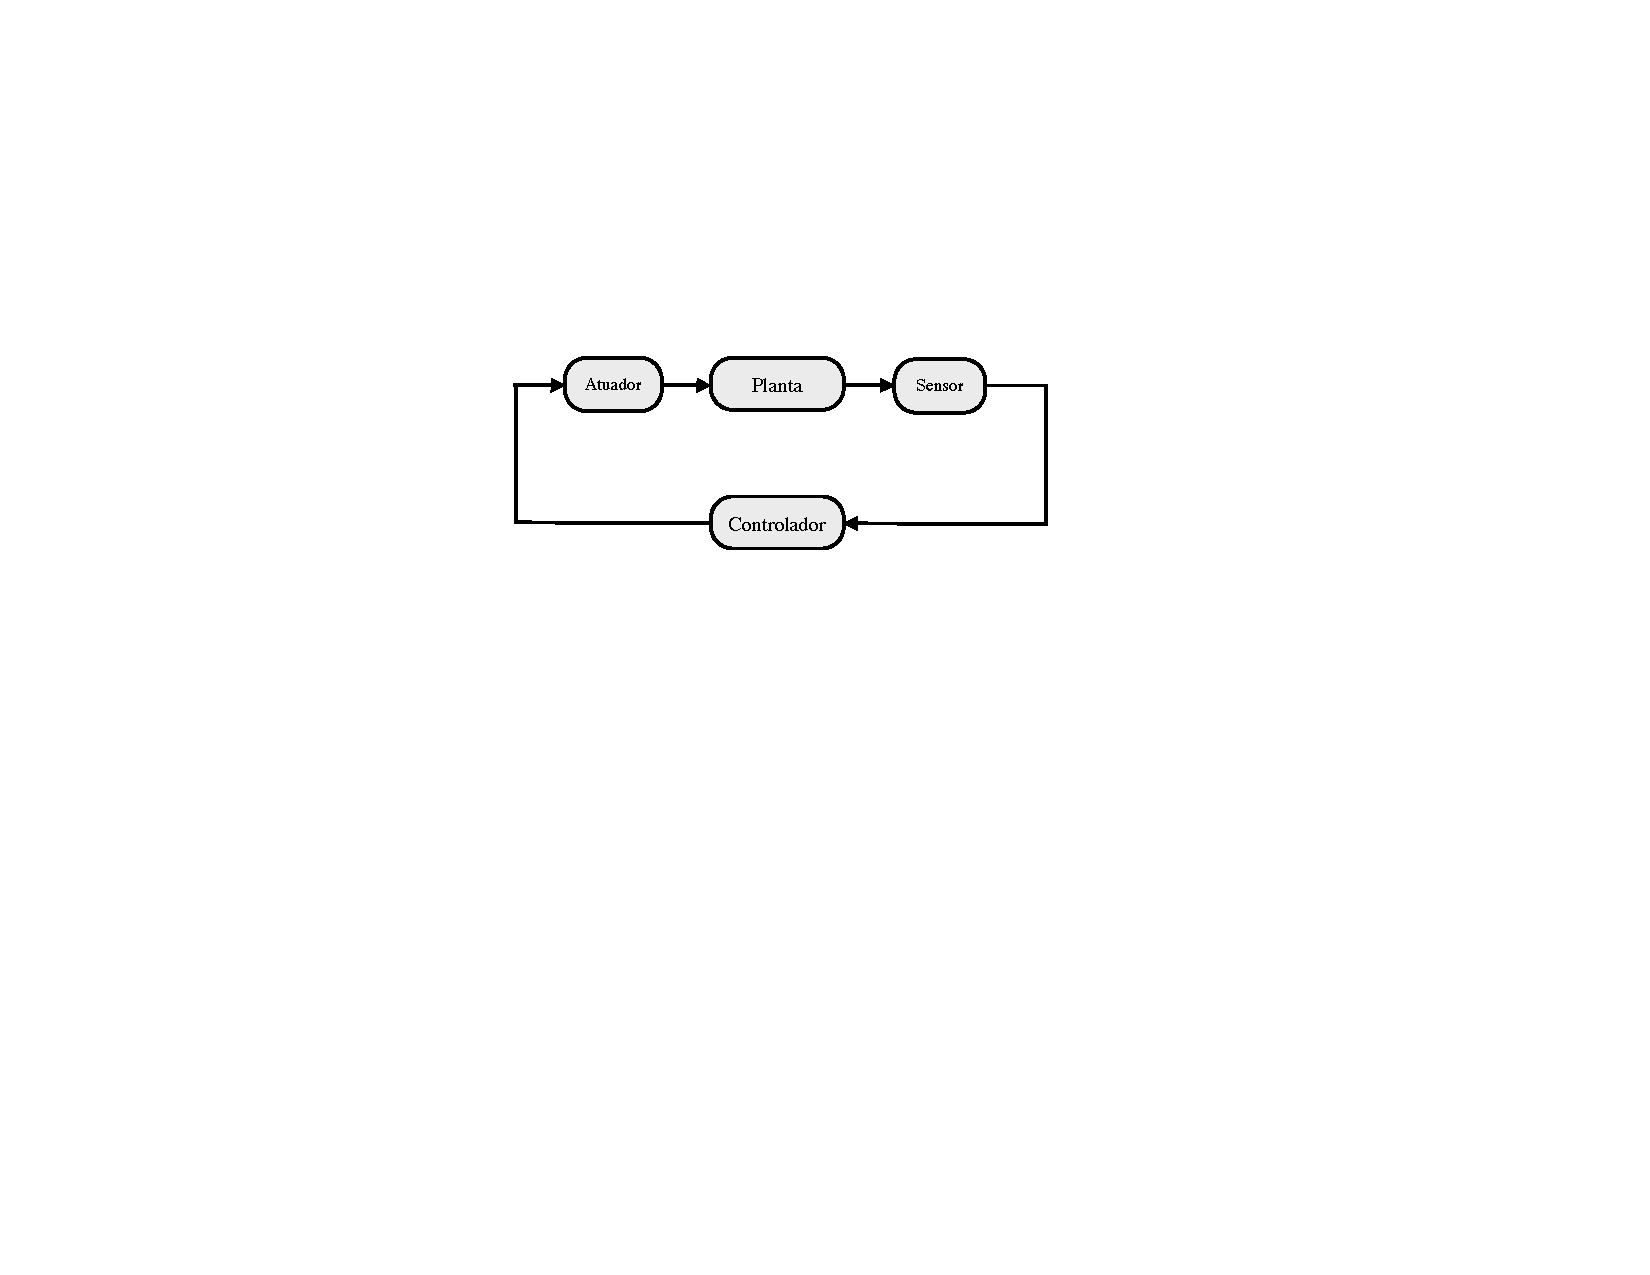
\includegraphics{DescricaoProcesso/Figuras/FiguraProcesso.pdf}}
  \caption{Aqui escrevemos \textbf{toda} informação pertinente à figura. Ou seja, este texto deve ser uma descrição auto-contida da figura, não sendo necessário recorrer ao corpo de texto para saber detalhes sobre a mesma. \emph{Fonte:} Citar fonte se figura 	não for elaborada pelo autor e \textbf{pedir permissão para usar!}}
  \label{fig:processo}
\end{figure}


\section{Situação Atual/Estado da Arte/Revisão da Literatura}
\label{sec:revisão}

Este é o espaço para uma revisão detalhada do enquadramento do problema. Isso inclui descrever a situação atual do processo, aquilo que foi feito até então dentro da empresa/laboratório, e aquilo que se pode chamar de ``Estado da Arte'', ou seja, uma apresentação do conhecimento preexistente
sobre o tema do projeto.

A elaboração desta seção tipicamente demanda uma boa revisão da literatura. Deve haver, quando aplicável uma análise das soluções potencialmente concorrentes, elencando vantagens e desvantagens.

\subsection{Como Elaborar uma Revisão da Literatura}

Ao selecionar referências, devem-se preferir referências de veículos confiáveis, que tenham por exemplo processo de revisão por pares. Portanto, dá-se preferência a artigos em periódicos e livros, em seguida teses e dissertações, artigos em anais de congresso e por fim relatórios. Evitar citar páginas da internet por oferecem menor garantia da informação nelas contida. 

Pesquise sua bibliografia em bases confiáveis como o \textsf{Web of Science}, \textsf{Scopus}, ou o \textsf{Google Scholar}. \textbf{Não use uma ferramenta de busca comum!} (elas não foram feitas pensando no \emph{ranking} de textos científicos) Use o número de citações de uma dada referência como um indicador de sua qualidade. Explore os artigos que citam a referência estudada bem como os artigos que ela cita.

Prefira as referências mais recentes quando se tratar de um assunto na fronteira do conhecimento ou de tecnologia de ponta. Quando se tratar de um assunto já consolidado, prefira citar livros ou artigos com muitas citações. 

Evite citar informações de segunda-mão e procure na medida do possível rastrear a fonte original. Contudo, em situações em que a fonte original é de acesso mais difícil, seja por ter tido publicação limitada como no caso de relatórios ou por não ser em língua inglesa ou portuguesa, é preferível a citação de segunda-mão em um veículo mais acessível.

Para gerenciar suas referências, use uma ferramenta de software como o \textsf{Mendeley}, que permite gerar arquivos .bib para uso em {\LaTeX} ou simplesmente gerar a lista de referências para uso direto em editores de texto. Em \LaTeX, mais especificamente Bib\TeX, a lista de referências é criada a partir de um arquivo .bib, que é uma espécie de banco de informações bibliográficas em que cada entrada é uma referência associada a uma chave para citação. A lista criada incluirá apenas as referências citadas ao longo do texto, mesmo que haja mais referências no arquivo .bib. As informações bibliográficas no formato Bib\TeX também podem ser obtidas para cada referência em ferramentas como o \textsf{Google Scholar} e então coladas no arquivo .bib.

Na Seção \ref{sec:comocitar} discutiremos como e quando as citações devem ser usadas.

\section{Resumo do Capítulo}

Tente não terminar de forma abrupta. Se for escrever algo aqui, não seja genérico!


\clearpage

\chapter{Metodologia}
\label{chap:metodologia}

Este capítulo deve descrever os métodos utilizados no projeto. As teorias e ferramentas utilizadas, assim como as ações executadas, devem ser escritas de forma clara e precisa, sem deixar espaço para ambiguidades. Tenha em mente que \textbf{o objetivo aqui é dar credibilidade ao seu trabalho e permitir que ele possa ser reproduzido por quem tenha interesse (algumas vezes por você mesmo!)}. 

É natural que este capítulo contenha uma revisão bibliográfica mais detalhada das técnicas utilizadas. O ideal é que o capítulo seja auto-contido, de modo que o leitor não necessite recorrer às referências para entender seu trabalho ou reproduzi-lo.

Ao apresentar os métodos, será importante justificar devidamente as opções tomadas e discutir as alternativas disponíveis e os critérios que o levaram à escolha do método.

No restante do capítulo, apresentamos um pequeno manual de escrita técnica.

\section{Técnica 1 - Organização do texto}
\label{sec:metodo1}

Procure \textbf{definir a estrutura} de seu texto \textbf{antes de começar a escrever}. Isso evitará que as ideias apareçam foram de ordem. A falta de organização é uma das características mais comuns de textos difíceis de ler.

Nunca invoque conceitos ou objetos antes de defini-los. Procure fornecer o máximo de informação \emph{a priori} possível. Evite referências para frente no texto. 

Para evitar que o leitor se perca, antes de iniciar um trecho longo de texto que contenha ideias diversas, \textbf{adiante para o leitor o que será feito}, aonde se quer chegar. Ao fim do trecho, declare explicitamente que chegou à conclusão que desejava. Esta técnica vale especialmente para seções e capítulos do texto. 

\section{Técnica 2 - Estilo}
\label{sec:estilo}

O texto técnico deve ser preciso, claro, sem ambiguidades, objetivo e conciso. Mesmo com esse rigor, não deixe de prender a atenção do leitor. Lembre-se de que o início e o fim de cada parágrafo, de cada frase, são as partes mais importantes e onde você deve colocar maior ênfase.


\subsection{Precisão}

Use as palavras corretas! Não escreva redondo se é esférico. Não escreva igual se é aproximado. Não escreva sistema se é função de transferência. Não escreva grande, pequeno, máximo, mínimo, ótimo, se não há uma escala que defina tais conceitos.

Prefira usar números que deem uma noção de escala a usar adjetivos difíceis de precisar.

Seja específico e evite generalidades. Por exemplo, em vez de dizer ``O processo 1 é um processo de alto custo'', devemos ser mais precisos com relação à natureza do custo e dizer ``O processo 1 possui custo operacional elevado com relação a processos tradicionais tais como o processo 2''.

\subsection{Clareza}

Não deixe margem para dúvidas! Para reduzir a possibilidade de confusão na leitura do seu texto, \textbf{evite frases longas}. Nunca escreva frases com mais de $20$ palavras. Procure escrever na média $12$ palavras por frase. Evite palavras compridas ou que possam ser consideradas difíceis.

Não deixe ideias subentendidas! Não assuma que seu leitor pensa como você e vai saber do que você está falando. Explicite todos os passos de seu raciocínio lógico. Pular passos de raciocínio é uma das causas mais comuns de confusão na leitura. Não seja preguiçoso neste quesito.

Novamente, defina todos os conceitos antes de fazer uso deles.

Não deixe o sujeito verbal subentendido. Para evitar ambiguidades, tome cuidado ao usar pronomes como ``esse, este, isso, ele''. É preferível repetir um nome a deixar margem para dúvidas. Por exemplo, após a primeira frase deste parágrafo poderíamos dizer de forma não tão clara: ``Esta é uma causa de confusão na escrita.''; ou poderíamos dizer de forma mais clara: ``Essa falta de informação é uma causa de confusão na escrita.''

Não há problemas em haver repetições em textos técnicos. O mais importante é a clareza, a inexistência de ambiguidades, não a beleza. Se acha que uma determinada frase pode ser confusa ou se alguma ideia parece difícil de explicar, repita a mesma ideia em outras palavras ou, melhor ainda, dê um exemplo.

Por fim, domine o significado das palavras utilizadas para evitar ambiguidades. Se uma palavra pode ter mais de um significado em determinada frase, tente trocá-la por outra que não deixe dúvidas. Mais importante ainda, não use palavras sobre cuja definição você não tem certeza.

\subsection{Ojetividade}

O texto técnico deve ser direto ao ponto, sem rodeios, e livre de opiniões. Evite apartes, evite divagações e discussões irrelevantes com relação ao tema principal.

\textbf{Nunca use hipérboles}. Cuidado com termos como ``otimizar, muito grande, enorme, muito bom''.  Usar números sempre que possível para quantificar conceitos, sejam eles precisos ou apenas uma estimativa. Em especial deve-se tomar cuidado com as palavras ``muito'' e ``muitos''.

O tom deve ser impessoal, apresentando apenas fatos e não opiniões. Em português, a voz passiva é um instrumento comum para se obter um tom impessoal. Contudo, sempre que possível, tente usar a voz ativa ou a voz passiva sintética para deixar o texto mais fluido e claro.

Palavras abstratas deixam a escrita vaga. Prefira palavras concretas, fortes, isto é, palavras que tenham um único significado. Sempre que possível substitua múltiplas palavras por uma única. Por exemplo, na frase ``A máquina processou as amostras'' temos duas palavras genéricas: máquina e processar. A mesma ideia seria mais objetiva se expressa como ``A centrífuga girou as amostras''.

Controle seu tom. \textbf{Não use linguagem coloquial. Não use clichês}. Não use de arrogância: ``obviamente, como é sabido, é claro que''. 

\subsection{Concisão}

O texto técnico deve ser tão curto quanto possível, sem prejuízo de sua clareza e precisão. Não use palavras a mais, não inclua expressões irrelevantes ou supérfluas. Não escreva simplesmente para encher as páginas. Se um assunto não é relevante para a compreensão do seu trabalho, corte-o, mova-o para um apêndice ou aponte uma referência.

Evite redundâncias como ``opinião pessoal'' e ``garantia absoluta''.

\section{Vícios comuns}

\begin{itemize}
\item Estrangeirismos: ``\emph{performance}'', ``\emph{mutatis mutandis}''. Se necessário, coloque o termo estrangeiro em itálico e dê uma tradução entre parênteses.

\item Usar linguagem rebuscada. Lembre-se de que a linguagem técnica deve ser clara, precisa e objetiva.

\item Alternar o tempo verbal entre passado e presente. Seja consistente e escreva apenas no passado ou no presente.

\item Iniciar uma frase com verbo porque o sujeito está implícito na frase anterior. Deixe sempre o sujeito explícito.

\item Inserir referências no meio de uma frase. Isso quebra o fluxo da leitura. Coloque a citação no fim da frase.

\item \textbf{Usar siglas sem antes defini-las}. Sempre escreva a sigla por extenso \emph{na primeira vez} que ela aparece no texto. Por exemplo, ``este é um texto de Projeto Final de Curso (PFC)''. 

\item Escrever ``como sabemos'', ``como é sabido'', ``por razões óbvias'', ``é evidente que'', ``talvez seja verdade que''. Estes termos significam apenas que você não sabe explicar o que está afirmando.

\item Usar definições \emph{por exemplo}, isto é, apresentar a definição de um conceito ou termo por meio de um exemplo. Primeiro defina o conceito, depois exemplifique.

\end{itemize}

\section{Boas práticas}

\begin{itemize}
\item Sempre que introduzir novos termos e conceitos, destaque-os em itálico para que o leitor saiba que se trata de uma definição e para que ele ache a definição com facilidade quando for necessário rastreá-la no texto.
\item Releia o que escreve a cada parágrafo. Releia rapidamente cada seção para verificar o encadeamento de ideias.
\item Corte palavras sempre que possível.
\item Nunca assuma que o leitor entenderá o que você escrever. Esforce-se para fazê-lo entender.
\item Use um corretor ortográfico.
\item Peça que alguém leia seu texto.
\end{itemize}


\section{Uso de referências}
\label{sec:comocitar}

Uma afirmação incluída num texto técnico se enquadra em um de três casos: a) seu conteúdo é de conhecimento geral dentro da área do texto; b) seu conteúdo é original e resulta do trabalho do autor; c) seu conteúdo tem origem em outro trabalho (ainda que seja do mesmo autor, não é original).

Toda afirmação enquadrada na categoria c) deve ser acompanhada de uma citação. Para afirmações da categoria b), deixe claro que se trata de ideia original do autor. Isso evita que o leitor se confunda ao pensar que possa se tratar de a) ou c).

No caso a), pode ser um tanto mais sutil determinar o que deve ser de conhecimento geral. Procure evitar o excesso de citações. Se todo um parágrafo se baseia em ideias de uma certa referência, em geral basta que ela seja citada no seu início.

\textbf{Atenção:} Não copie frases das referências usadas. Reescreva as ideias com suas próprias palavras e não deixe de citar a fonte. Se for necessário manter as palavras do original, cite a frase entre aspas e em itálico.

\section{Honestidade e Plágio}

Seja honesto ao escrever. \textbf{Não ``maqueie'' seus resultados}. Não apresente apenas as melhores amostras dos seus resultados para dar a impressão de que foi bem sucedido. Não escreva aquilo que não entende. Não escreva de forma vaga para mascarar o fato de que não entende algo.

Dê crédito a quem o merece. Inclua referências sempre que usar o trabalho de outros. Seja sempre claro para não dar a impressão de que fez algo feito por outrem. \textbf{Não assuma crédito pelo trabalho dos outros}. Isso pode ter implicações legais e acadêmicas.

\section{Cuidado com a gramática}

\begin{itemize}

\item Erros gramaticais deixam uma \textbf{impressão ruim} e podem alterar a disposição do leitor para com o texto.  

\item Use a vírgula corretamente. Seu uso incorreto confunde o leitor. Nunca use a vírgula porque acha que a frase precisa de uma pausa. Não separe sujeito e verbo. Quando há inversão da ordem natural em uma frase, \emph{toda} a parte movida deve estar entre vírgulas.

\item Cuidado com a concordância da voz passiva sintética. Lembre-se de que o correto é ``Vendem-se ovos'' e não ``Vende-se ovos''.

\item Use a crase corretamente. Faça sempre o exercício de substituir o nome que sucede o ``à'' por um nome no masculino. Se o correto for usar ``ao'' com o nome masculino, então deve haver crase. Nunca use crase antes de nomes no masculino!

\item Escreva ``em que'' em vez de ``onde'' quando não houver indicação de lugar.

\item Não se escreve ``o fato \textbf{dela} ser'' ou ``a razão \textbf{do} texto ser escrito''. Escreve-se ``o fato \textbf{de ela} ser'' e ``a razão \textbf{de o} texto ser escrito''.

\item Releia o que escreve e na dúvida busque ajuda.

\end{itemize}

\section{Resumo do Capítulo}
\label{sec:metodo1b}

Tente não terminar de forma abrupta. Se for escrever algo aqui, não seja genérico!


\clearpage
\chapter{Resultados}

Para a execução do projeto, algumas etapas de desenvolvimento tiveram de ser seguidas: familiarização com o sistema, estudo dos módulos envolvidos, leitura dos requisitos, elaboração de documento descrevendo todo o processo de implementação e relacionamento com os diversos módulos, implementação e testes.


\section{Atividades do Projeto}
\label{metodo3}

\section {Requisitos do Sistema}
\label{req}


\section{Desenvolvimeto e Implementação}

A Tabela \ref{tab:tabela} apresenta as atividades executadas.

\begin{table}
\centering
%Note os alinhamentos diferentes em cada coluna
\begin{tabular}{|c|r|l|}\hline
		Atividade 1 & aa  & ab  \\ 
					 & a & b \\ \hline
		Ativ. 2  & aa & ab \\			
					 &  a & b \\ \hline
		\end{tabular}
	\caption{Exemplo de tabela - Coloque toda informação sobre a tabela aqui}
	\label{tab:tabela}
\end{table}

\section{Testes}

\section{Análise dos Resultados}

Apresente os resultados sem adulterações e faça análises objetivas. Pense na melhor maneira de apresentar os resultados graficamente. Se os gráficos são difíceis de interpretar, talvez tabelas sejam uma forma melhor de apresentar resultados. Não apresente dados (gráficos e tabelas) se não há uma conclusão interessante a ser tirada. Lembre-se de ser conciso.

\emph{Não se esqueça das unidades!} Pense que \emph{a priori} todo número deve ter uma unidade. Não escreva as unidades em itálico (no ambiente matemático) e tome cuidado para diferenciar maiúsculas e minúsculas. Um exemplo é escrever $22$ [kN] e não $22 KN$ (Kelvin vezes Newton!).

Ao apresentar resultados experimentais, tome o cuidado para também apresentar o cálculo das incertezas sempre que forem significativas. Ao fazer conclusões, sempre considere se o tamanho da sua amostra é grande o suficiente do ponto de vista estatístico. Lembre que a média empírica $\hat{\mu}_X$ de $N$ observações independentes da variável $X_i$ possui variância
\[
\hat{\sigma}_{\mu}^2 = \frac{1}{N(N-1)} \sum_{i=1}^N (X_i-\hat{\mu}_X)^2
\enspace,
\]
onde se assume que as variáveis $X_i$ possuem uma mesma ditribuição e que essa distribuição possui segundo momento finito.


\section{Resumo do Capítulo}
\label{sec:resumoo4}
Tente não terminar de forma abrupta. Se for escrever algo aqui, não seja genérico!

\section{Formato, expressões matemáticas e o \LaTeX}

\subsection{O \LaTeX}

O {\LaTeX}  é o método preferencial de preparação de documentos para textos técnicos nas ciências exatas. O {\LaTeX} permite não só lidar com equações de uma forma mais prática que em editores de texto, mas também facilita a formatação de documentos e tem um desempenho marcadamente superior a editores de texto na preparação de documentos longos como monografias. 

Documentos em {\LaTeX} são escritos em um ou mais arquivos de texto com extensão .tex. Após a escrita, o .tex é \emph{compilado} para gerar arquivos nos formatos .pdf, .dvi ou .ps. Hoje há duas distribuições padrão para o \LaTeX. Sistemas Windows usam o {Mik\TeX} e sistemas Unix usam o \TeX Live. Além das distribuições, muitos usuários utilizam \emph{front-ends} que facilitam a edição do texto, a compilação e a instalação de pacotes. 

Os pacotes necessários para compilar o presente documento devem ser encontrados numa instalação completa dessas distribuições. Se tiver dificuldades com os pacotes, você pode instalá-los manualmente ou tentar alterar o código para usar versões antigas dos mesmos.

A compilação pode ser feita pelos comandos \textsf{latex} ou \textsf{pdflatex}, invocados pela linha de comando ou pelo \emph{front-end}. Note que será necessário empregar o comando \textbf{mais de uma vez} para que as referências cruzadas saiam corretas.

Como discutido na Seção \ref{sec:revisão}, uma ferramenta útil para gerenciar as citações em {\LaTeX} é o Bib\TeX. Para gerar uma lista bibliográfica a partir do arquivo .bib, este arquivo deve ser indicado no arquivo .tex. Em seguida devem-se executar os comandos \textsf{pdflatex}, \textsf{bibtex} e \textsf{pdflatex} novamente sempre usando o .tex como argumento. Note que os comandos são executados nesta ordem e de forma repetida para que as referências cruzadas sejam geradas corretamente.

Nesta seção você deve encontrar exemplos dos comandos mais usados em \LaTeX. Outros exemplos e manuais podem ser encontrados na internet com facilidade.

\subsection{Expressões Matemáticas}

Ao escrever expressões matemáticas, defina todas as variáveis antes de usá-las ou imediatamente depois da expressão. Deixar de fazê-lo torna seu texto \textbf{ilegível}. Segue um exemplo.

Seja o par $(a_1,a_2)\in \mathbb{R}^2$. Para $s\in\mathbb{C}$, definimos a função $f(s)$ como
\[%cria equações sem numeração
f(s)\triangleq \frac{a_1 s+a_2}{s^2+2\zeta\omega_n s+\omega_n^2}
\enspace,
\]
onde os escalares $\zeta,\omega_n>0$ são constantes.

Note que não foi necessário atribuir valores às variáveis neste momento. Repare também como devemos \textbf{usar pontuação} (vírgula) nas equações, tratando-as como parte da frase. Usamos o símbolo $\triangleq$ ou $:=$ para deixar explícito que se trata de uma definição. Ser claro nesse aspecto facilita o entendimento do leitor.

A equação acima não foi numerada porque não será citada no texto. Vejamos um exemplo com numeração.

A função $f(\cdot)$ possui um zero em $-a_2/a_1$ (ou $-\frac{a_2}{a_1}$) e, para $\zeta<1$, possui polos complexos $p_{1,2}$ dados por
\begin{equation}
\label{eq:polos}
p_{1,2}=\omega_n \left(-\zeta\pm j\sqrt{1-\zeta^2}\right)
\enspace.
\end{equation}
Agora podemos citar os polos dados pela Equação (\ref{eq:polos}) (aqui adotamos a convenção de citar sempre com o número entre parênteses precedido da palavra Equação). Note como usamos um comando especial na Equação \ref{eq:polos} para garantir o ajuste automático do tamanho dos parênteses.

Vejamos agora como criar equações alinhadas. Considere o sistema dinâmico dado pelas equações diferenciais:

\begin{align}
\dot{x}_1 & = \cos(x_2)\cdot\ln(1/x_1)+\tan(u) \label{eq:x1dot} \\
\dot{x}_2 & = e^{-x_1-x_2} \nonumber \\
& y  = \min\{x_1,x_2\}  \label{eq:saida}
\enspace,
\end{align}
onde $x(t)=[x_1(t) ~ x_2(t)]'$, $t>0$, é a variável de estado do sistema, $u(t)$ é o sinal de entrada e $y(t)$ é o sinal de saída do sistema. Note no .tex que o caracter de tabulação \textsf{\&} foi usado para indicar o ponto de alinhamento horizontal das equações. Além disso, para ilustrar o uso do \LaTeX, retiramos a numeração da segunda equação e citamos as equações separadamente.

Nas Equações (\ref{eq:x1dot}) e (\ref{eq:saida}), aparecem operadores como $\min$, $\ln$, $\cos$ e $\tan$. A convenção aqui é que \textbf{variáveis devem ser escritas em itálico e operadores não}. Por essa razão todas as expressões matemáticas devem ser escritas no ambiente matemático (entre cifrão) mesmo quando for possível usar texto comum. Isso garante a consistência das fontes utilizadas (nem sempre a fonte do ambiente matemático é a mesma fonte do texto). 

Para escrever matrizes, podemos fazer por exemplo:
\[
\sum_{n=0}^{\infty}z^{-n}\left[\begin{array}{cc}
\lambda & 1 \\
0 & \lambda
\end{array}\right]^n=
\left[\begin{array}{cc}
\frac{z}{z-\lambda} & \frac{z}{(z-\lambda)^2} \\
0 & \frac{z}{z-\lambda}
\end{array}\right]
,~\forall \lambda<|z|
\enspace.
\]

Para escrever uma expressão com múltiplos casos, podemos fazer, para um inteiro $N$ positivo,
\[
g[n]=
\left\{
\begin{array}{ll}
0,& \mbox{se }~ n\leq 0 \\
n,& \mbox{se }~ n=1,2,\ldots,N-1 \\
N,& \mbox{se }~ n\mod N = 0 \\
0,& \mbox{caso contrário}\enspace.
\end{array}
\right.
\]

\textbf{Nunca reaproveite símbolos} matemáticos, isto é, nunca use o mesmo símbolo para designar variáveis diferentes.

Para um exemplo com múltiplas linhas de expressão matemática: tem-se que, para $a\neq 0$,

\begin{equation}
\begin{split}
ax^2+bx+c &= 0 \\
& \Rightarrow a(x^2+bx/a+c/a) =0 \Rightarrow a((x+b/(2a))^2+c/a-b^2/(4a^2))=0  \\
& \Rightarrow (x+b/(2a))^2=(b^2-4ac)/(4a^2) \\
& \Rightarrow (x+b/(2a))=\pm\sqrt{b^2-4ac}/(2a) \\
& \Rightarrow x=\frac{-b\pm\sqrt{b^2-4ac}}{2a}
\enspace.
\end{split}
\end{equation}

Note a argumentação lógica aqui. Não estamos dizendo que o valor de $x$ é dado pela última linha. Estamos dizendo que a hipótese da primeira linha juntamente com a hipótese $a\neq 0$ implicam os referidos valores de $x$. \textbf{Um erro comum dos alunos ao escrever é não distinguir a veracidade das implicações com a veracidade das hipóteses}.

\clearpage
\chapter{Conclusões}

Novamente, este será um dos trechos que o leitor experiente lerá antes de decidir se vale a pena ler o texto integral. Seja convincente.

\section{Considerações Finais}

Reitere o que de mais importante foi feito, qual era o objetivo inicial e qual o resultado obtido. Se houve requisitos ou especificações de projeto, discuta se foram atingidos. Se os resultados não foram conclusivos ou contrariam o que se esperava, seja honesto e diga-o explicitamente. Busque explicar os insucessos com argumentos sólidos e plausíveis. 

\section{Propostas de Continuidade}

Se houve questões ainda não respondidas ou resultados insatisfatórios, aponte direções de continuação.

\clearpage


\addcontentsline{toc}{chapter}{Referências Bibliográficas}
\renewcommand{\bibname}{Referências Bibliográficas}

%\bibliographystyle{abntex2-alf} %para norma ABNT no sistema autor-data
\bibliographystyle{abntex2-num}
\begin{small}
\bibliography{ListadeReferencias}%,library}
%% Monografia para Projeto de Fim de Curso - Exemplo no LaTeX
%-----------------------------------------------------------


%---------------Inicialização de pacotes--------------------

\documentclass[12pt,a4paper,notitlepage,twoside]{book}


\usepackage{graphicx}
\usepackage[utf8]{inputenc}
%\usepackage[latin1]{inputenc} %%pode ser necessário trocar a codificação em sistemas Windows
\usepackage[brazil]{babel}		%%pode ser necessário trocar o pacote de línguas em algumas distribuições LateX
%\usepackage[portuguese]{babel}
\usepackage[T1]{fontenc}
\usepackage{amsmath,amssymb}
\usepackage{amsthm,amsfonts}
\usepackage{color}
\usepackage[colorlinks]{hyperref}
\usepackage{abntex2abrev}
%\usepackage[alf]{abntex2cite} %se você quiser seguir as normas ABNT no sistema autor-data
%\usepackage[num]{abntex2cite} %se você quiser seguir as normas ABNT no sistema numérico
\usepackage{setspace}
\usepackage[toc,page]{appendix}

%Definindo fonte Times (Use os pacotes obsoletos se não conseguir instalar os atualizados)
%\usepackage{times}     %Pacote de fontes obsoleto, apenas texto
%usepackage{mathptmx}  %Pacote de fontes obsoleto, texto e símbolos matemáticos
%\usepackage{newtxtext,newtxmath}  %Pacotes de fontes mais recentes

\usepackage[a4paper,top=30mm,bottom=30mm,inner=30mm,outer=25mm,headheight=7mm,headsep=6mm,footskip=7mm]{geometry}
\usepackage{enumerate}

\makeindex

%\singlespacing   %%espaçamento simples
%\onehalfspacing
%\setstretch{1.03} %%um pouco melhor que espaçamento simples
\linespread{1.25} %corresponde ao espaçamento 1.5 do MS Word

%---------------Início do documento-------------------------

\begin{document}

\include{Capa/capa}

\pagenumbering{roman}
\include{Resumo/Resumo}
\include{Resumo/Abstract}
\include{Agradecimentos/Agradecimentos}
\include{TabelaConteudo/TabelaConteudo}
\include{ListaFiguras/ListaFiguras}
\include{ListaTabelas/ListaTabelas}

\pagenumbering{arabic}
\setcounter{page}{1}
\include{Introducao/Introducao}
\include{DescricaoProcesso/DescricaoProcesso}
\include{Metodologia/Metodologia}
\include{Resultados/Resultados}
\include{Conclusao/Conclusao}

\addcontentsline{toc}{chapter}{Referências Bibliográficas}
\renewcommand{\bibname}{Referências Bibliográficas}

%\bibliographystyle{abntex2-alf} %para norma ABNT no sistema autor-data
\bibliographystyle{abntex2-num}
\begin{small}
\bibliography{ListadeReferencias}%,library}
%\input{Monografia.bbl}
\end{small}

%\begin{appendices}
\appendix
\include{Apendices/ApendiceA}
\include{Apendices/ApendiceB}
%\end{appendices}

\end{document}

%---------------Fim do documento----------------------------
\end{small}

%\begin{appendices}
\appendix
\chapter{Trials and failures}

\section{Machine Learning}

I've tried to create a database with the samples of current. Each sample was a vector with 50k values corresponding a 0.5s of data collected in a 100KHz oscilloscope. And in a second column its 



\subsection{Spectogram analysis}

\begin{figure}[H]
    \center
    \includegraphics[width=3cm]{Figuras/spectogram/5_Dripping.png}
    \label{fig:spectrogram1}
    \caption{Dripping}
  \end{figure}

%   \begin{figure}[H]
%     \center
%     \includegraphics[width=3cm]{Figuras/spectogram/5_Dripping.png}
%     \label{fig:spectrogram1}
%     \caption{Dripping}
%   \end{figure}
  

\chapter{O que mais faltou}

Inclua aqui informações que não sejam tão relevantes para o entendimento do projeto mas que ainda sejam importantes para documentá-lo. 


Foto e detalhes dos instrumentos

\begin{figure}[H]
    \centering
    \resizebox{150mm}{!}{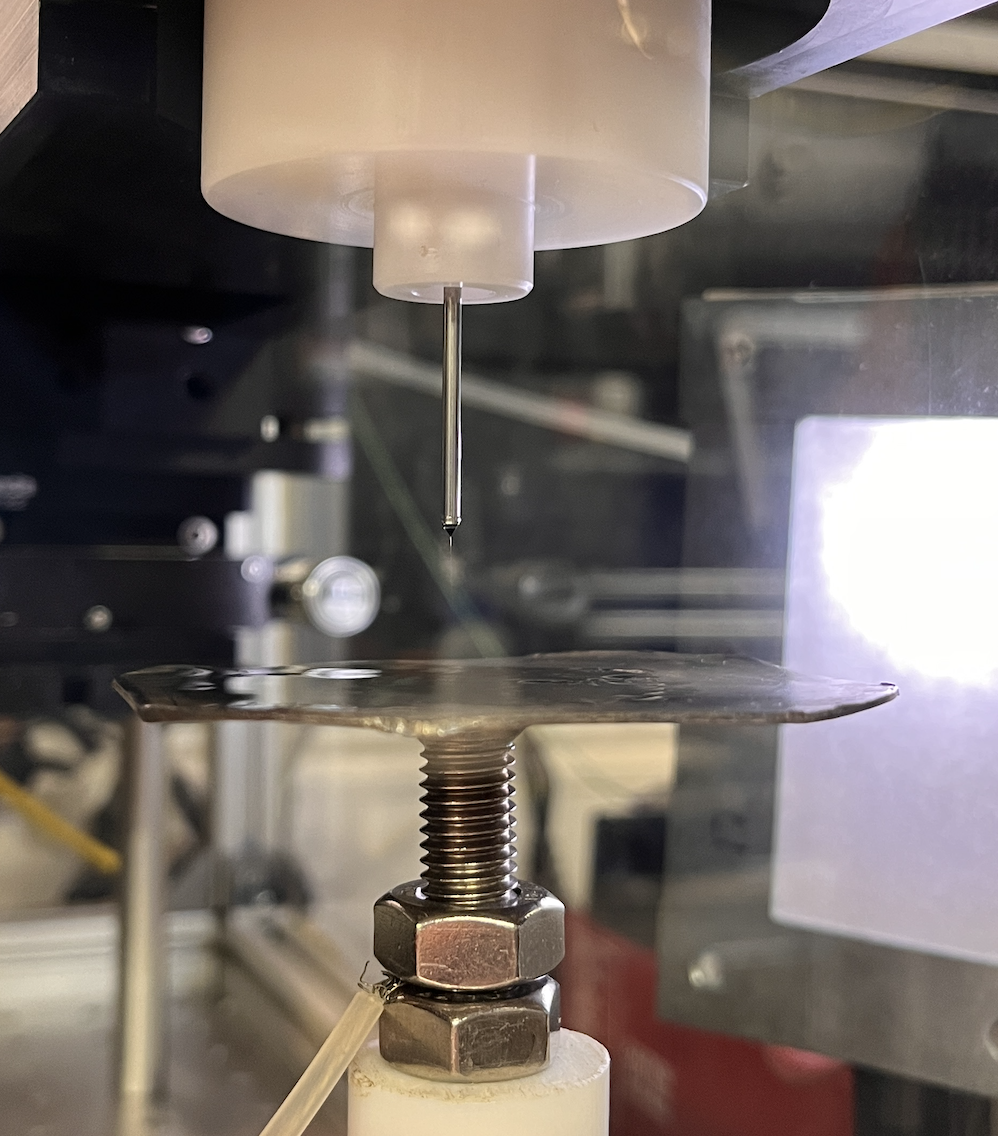
\includegraphics{Figuras/naked_eyes.png}}
    \caption{EHDA physical concept }
\end{figure}



%\end{appendices}

\end{document}

%---------------Fim do documento----------------------------
\end{small}

%\begin{appendices}
\appendix
\chapter{Trials and failures}

\section{Machine Learning}

I've tried to create a database with the samples of current. Each sample was a vector with 50k values corresponding a 0.5s of data collected in a 100KHz oscilloscope. And in a second column its 



\subsection{Spectogram analysis}

\begin{figure}[H]
    \center
    \includegraphics[width=3cm]{Figuras/spectogram/5_Dripping.png}
    \label{fig:spectrogram1}
    \caption{Dripping}
  \end{figure}

%   \begin{figure}[H]
%     \center
%     \includegraphics[width=3cm]{Figuras/spectogram/5_Dripping.png}
%     \label{fig:spectrogram1}
%     \caption{Dripping}
%   \end{figure}
  

\chapter{O que mais faltou}

Inclua aqui informações que não sejam tão relevantes para o entendimento do projeto mas que ainda sejam importantes para documentá-lo. 


Foto e detalhes dos instrumentos

\begin{figure}[H]
    \centering
    \resizebox{150mm}{!}{\includegraphics{Figuras/naked_eyes.png}}
    \caption{EHDA physical concept }
\end{figure}



%\end{appendices}

\end{document}

%---------------Fim do documento----------------------------
\end{small}

%\begin{appendices}
\appendix
\chapter{Trials and failures}

\section{Machine Learning}

I've tried to create a database with the samples of current. Each sample was a vector with 50k values corresponding a 0.5s of data collected in a 100KHz oscilloscope. And in a second column its 



\subsection{Spectogram analysis}

\begin{figure}[H]
    \center
    \includegraphics[width=3cm]{Figuras/spectogram/5_Dripping.png}
    \label{fig:spectrogram1}
    \caption{Dripping}
  \end{figure}

%   \begin{figure}[H]
%     \center
%     \includegraphics[width=3cm]{Figuras/spectogram/5_Dripping.png}
%     \label{fig:spectrogram1}
%     \caption{Dripping}
%   \end{figure}
  

\chapter{O que mais faltou}

Inclua aqui informações que não sejam tão relevantes para o entendimento do projeto mas que ainda sejam importantes para documentá-lo. 


Foto e detalhes dos instrumentos

\begin{figure}[H]
    \centering
    \resizebox{150mm}{!}{\includegraphics{Figuras/naked_eyes.png}}
    \caption{EHDA physical concept }
\end{figure}



%\end{appendices}

\end{document}

%---------------Fim do documento----------------------------